%% Latex template for PhD dissertation or MS thesis
%% Department of Electrical and Computer Engineering
%% Brigham Young University
%% Last Modified: July 2017 by mdr@byu.edu

\documentclass[12pt,oneside]{report}
% generate the one-sided version: this is the ETD version
% print the one-sided version one sided for all the department and college approvals

% \documentclass[12pt,twoside]{report}
% Uncomment this line (and comment line 6) to create the two-sided version.
% Print the two-sided version two-sided for the optional printed and bound version.

%%%%%%%%%%%%%%%%%%%%%%%%%%%%%%%%%%%%%%%%%%%%%%%%%%%%%%%%%
%  Setup BYU thesis format
%%%%%%%%%%%%%%%%%%%%%%%%%%%%%%%%%%%%%%%%%%%%%%%%%%%%%%%%%
\usepackage{byustyle}
% Setup the byu style sheet
\byustylesetup{%
	%
	isdissertation = false,            % false for MS thesis, true for PhD dissertation
	%
	% Definitions of names needed in thesis/dissertation
	deptname          = Department of Electrical and Computer Engineering,
	committeechairman = Brent E. Nelson,
	committeemembera  = Aaron R. Hawkins,
	committeememberb  = Brian A. Mazzeo,
	committeememberc  = Brad L. Hutchings, % needed for dissertation, ignored for thesis
	committeememberd  = Steven M. Schultz,    % needed for dissertation, ignored for thesis
	%
	%Change true/false to shorten for proofreading purposes
	noabstract = false,         % Do not show the abstract page
	nouniversitypages = false,  % Do not show any of the "university pages"
	noacknowledgements = false, % Do not show the Acknowledgements page
	notableofcontents = false,  % Do not show the Table of Contents
	nolistoffigures = false,    % Do not show the List of Figures
	nolistoftables = false,     % Do not show the List of Tables
	nonomenclature = true,      % Do not show the Nomenclature section - note that this section is optional
	notocandlists = false,      % Do not show the Table of Contents, List of Figures, or the List of Tables
	noheaderatall = false,      % Do not show any of the BYU Thesis header pages
	keywords = {thesis template, dissertation template, technical writing} % your keywords
}

%%%%%%%%%%%%%%%%%%%%%%%%%%%%%%%%%%%%%%%%%%%%%%%%%%%%%%%%
% Package inclusions go here
% The list starts with some commonly used packages
% That do not conflict with byutyle.sty
%%%%%%%%%%%%%%%%%%%%%%%%%%%%%%%%%%%%%%%%%%%%%%%%%%%%%%%%

\usepackage{amsmath}					%	allows for mathematical symbols
\usepackage{amssymb}					%	defines symbol names for all the math symbols
\usepackage{graphicx}        			% for .pdf graphics inclusion
\usepackage[calcwidth = \columnwidth]{caption}
\usepackage{booktabs,threeparttable}
\usepackage{setspace}					%	change the spacing inside a document
\usepackage{epstopdf}					%	converts a .eps to a .pdf
\usepackage{cite}						%	allows for citations
\usepackage{float}						%	improves the interface for defining floating objects
\usepackage{rotating}
\usepackage{printlen}
\usepackage{subcaption}

%%%%%%%%%%%%%%%%%%%%%%%%%%%%%%%%%%%%%%%%%%%%%%%%%%%%%%%%%%%%%%%%%%%%
%  Include additional \usepackage{} statements here.
%    Add one package at a time.
%    Warning:  Some packages are not compatible with byustyle.sty
%%%%%%%%%%%%%%%%%%%%%%%%%%%%%%%%%%%%%%%%%%%%%%%%%%%%%%%%%%%%%%%%%%%

%These next two lines are for the citing with the IEEE style
\renewcommand\citepunct{], [}
\renewcommand\citedash{]--[}
\newcommand\norm[1]{\left\lVert#1\right\rVert}

%%%%%%%%%%%%%%%%%%%%%%%%%%%%%%%%%%%%%%%%%%%%%%%%%%%%%%%%
% For doing bookmarks in the PDF file
%%%%%%%%%%%%%%%%%%%%%%%%%%%%%%%%%%%%%%%%%%%%%%%%%%%%%%%%%
% For more info, see:
% http://www.geocities.com/kijoo2000/latex2pdf.pdf
% http://www.tug.org/applications/hyperref/manual.html
\usepackage[pdftex,backref,pagebackref,plainpages=false]{hyperref}
\hypersetup{
    %bookmarks    = true, % Make bookmarks (default=true). This option
                          %cannot be used after package has been loaded,
                          %thus use like this: \usepackage[bookmarks=false]{hyperref}.
    %
    breaklinks   = false, % Allow link text to break across lines (default=false).
    linktocpage  = false, % make page number, not text, be link on TOC, LOF and LOT
    colorlinks   = false, % Color the text of links (true) or put color frames over
    %
    linkbordercolor  = {1 1 1}, % The color of the box around normal links (white so they won't show up)
    citebordercolor  = {1 1 1}, % The color of the box around citations (white so they won't show up)
                          % the links (false).
    pdfstartview = {FitV}, % Set the startup page view. Possible options are:
                           % FitH: Fit whole width of page
                           % FitV: Fit whole height of page
                           % FitB: Fit whole �Bounding Box� page
                           % FitBH: Fit whole width of �Bounding Box� of page
                           % FitBV: Fit whole height of �Bounding Box� of page
    bookmarksnumbered  = true, % Put section numbers in bookmarks (default=false)
    bookmarksopen      = true, % Open up the bookmark trees (default=false).
    bookmarksopenlevel = 0, % Level to which bookmarks are open (default=\maxdimen).
    bookmarkstype      = toc, % Specify which toc file to mimic (default=toc).
    pdfpagemode        = {UseOutlines}, %  Specify how document starts when opened ({None}).
                                        % Possible options are:,
                                        % None: Neither bookmarks nor thumbnails are visible.
                                        % UseOutlines: Bookmarks are visible.
                                        % UseThumbs: Thumbnails are visible.
                                        % FullScreen: Full-screen mode
    pdftitle    = {Thesis},
    pdftitle    = {First Line of your Thesis/Dissertation Title},
    pdfauthor   = {Isaac Newton},
    pdfcreator  = {Isaac Newton},
    pdfsubject  = {Isaac Newton's Master's Thesis},
    pdfkeywords = {Master's Thesis, BYU},
    pdfborder		=	{0 0 0},
    colorlinks=true,
    urlcolor=blue,
}

%%%%%%%%%%%%%%%%%%%%%%%%%%%%%%%%%%%%%%%%%%%%%%%%%%%%%%%%
%  Define macros here - You may use these, or delete them, as you see fit.
%%%%%%%%%%%%%%%%%%%%%%%%%%%%%%%%%%%%%%%%%%%%%%%%%%%%%%%%%

% \def\proof{\noindent{\it Proof: }}
% \def\QED{\mbox{\rule[0pt]{1.5ex}{1.5ex}}}
% \def\endproof{\hspace*{\fill}~\QED\par\endtrivlist\unskip}
% \newcommand{\norm}[1]{\left\|#1\right\|}
\newcommand{\abs}[1]{\left|#1\right|}
% \newcommand{\defeq}{\stackrel{\triangle}{=}}
% \newcommand{\re}{\mathbb{R}} 		% real numbers
% \newcommand{\OMIT}[1]{{}} 		% omit sections of text
\newcommand{\pd}[2]{\ensuremath{\frac{\partial #1}{\partial #2}}} % partial derivative
% \newcommand{\superscript}[1]{\ensuremath{^\textrm{#1}}}
% \newcommand{\subscript}[1]{\ensuremath{_\textrm{#1}}}


%%%%%%%%%%%%%%%%%%%%%%%%%%%%%%%%%%%%%%%%%%%%%%%%%%%%%%
% Define the 'inverted pyramid' table caption
% requirement from the College.
%%%%%%%%%%%%%%%%%%%%%%%%%%%%%%%%%%%%%%%%%%%%%%%%%%%%%%

\DeclareCaptionJustification{InvertedPyramid}{\hsize=\linewidth
                \parindent=0pt
                \leftskip=0pt plus.5fil
                \rightskip=0pt plus-0.5fil
                \parfillskip=0pt plus1fil
                \emergencystretch=1in
                \parshape10
                0.00in \linewidth
                0.025\linewidth 0.95\linewidth
                0.05\linewidth 0.9\linewidth
                0.075\linewidth 0.85\linewidth
                0.1\linewidth 0.8\linewidth
                0.125\linewidth 0.75\linewidth
	     0.15\linewidth 0.70\linewidth
	     0.175\linewidth 0.65\linewidth
	     0.2\linewidth 0.60\linewidth
	     0.225\linewidth 0.55\linewidth
                \strut
	} 
\renewcommand{\TPTminimum}{3in}
\captionsetup[table]{justification=InvertedPyramid} 

\newsavebox{\tempbox}
\newlength{\tempwidth}

%%%%%%%%%%%%%%%%%%%%%%%%%%%%%%%%%%%%%%%%%%%%%%%%%%%%%%%%%%%%%%%%%%%%
% To only print a few chapters without changing the reference numbers
% (Consult your favorite LaTeX resource.) 
%%%%%%%%%%%%%%%%%%%%%%%%%%%%%%%%%%%%%%%%%%%%%%%%%%%%%%%%%%%%%%%%%%%%
%\includeonly{...}

%%%%%%%%%%%%%%%%%%%%%%%%%%%%%%%%%%%%%%%%%%%%%%%%%%%%%%%%
% Start Document
%%%%%%%%%%%%%%%%%%%%%%%%%%%%%%%%%%%%%%%%%%%%%%%%%%%%%%%%
\begin{document}

% Define Title
% For a title of more than one line, use the \\ to break up the lines so they appear in an inverse pyramid shape.
% Also, make sure you use title case 
\title{On Writing an MS Thesis\\Second Line of Title if Necessary\\Three Line Limit}

% Define author
\author{Jae Hun Lee}

% For displaying the BYU Thesis header
% 	This command assumes that there are documents called abstract.tex and
% 	acknowledgements.tex (and optionally nomenclature.tex) that will be 
%   included in the header

\showBYUHeader

% Include chapters of the thesis here: 
% The inludes are populated by example chapters
\chapter{Introduction}

\section{Gimbal Control}

\section{Autonomous Target Following System}

\section{Unit Vector UAV Control}
\chapter{Gimbal Control}
\label{chp:chapter2}
\graphicspath{{figures/}{figures/chapter2/}}
Gimbals are widely used device for flying drones with a camera because they stabilize the camera from vibration and movement of the platform. Stabilizing the camera is important in order to take high-quality, smooth videos and photos. For this reason, most of the high-end commercial drones are equipped with a gimbal. For autonomous systems, a gimbal becomes more important because it adds maneuverability to the camera to provide more visual awareness and to keep the object of interest in the camera field of view. There are two cases when the object of interest can be centered on the optical axis. The first is when we know the relative location of the target to the camera. The second is when we know the target location in the image. For many practical applications, it is not feasible to assume that we know the target location in the global frame. Thus, image-based gimbal control is the more practical and realistic way to achieve the goal. In this chapter, we introduce several image-based gimbal control schemes.

\begin{figure*}[htbp]
    \centering
    \begin{subfigure}[t]{0.5\textwidth}
    	\centering
    	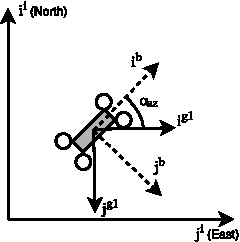
\includegraphics[width=2in]{images/chapter2/gimbal1_frame}
    	\caption{Top view to show the relationship between the body frame and the gimbal-1 frame}
    \end{subfigure}%
    ~
    \begin{subfigure}[t]{0.5\textwidth}
    	\centering
    	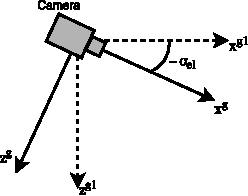
\includegraphics[width=2in]{images/chapter2/gimbal_frame}
    	\caption{Side view to show the relationship between the gimbal-1 frame and the gimbal frame}
    \end{subfigure}
    \caption{Frames of interest: body frame, gimbal-1 frame, and gimbal frame}
    \label{gimbal_frame}
\end{figure*}

\section{Angle Commanding Gimbal Control}
\subsection{Coordinate Frame Convention and Projective Camera Geometry}
Before giving a detailed explanation of the gimbal control algorithms, we describe the coordinate frame convention and projective camera geometry. Note that the coordinate frame convention follows the convention from chapter 13 of \cite{beard2012small}. We assume that the origins of the gimbal and camera frames are at the center of mass (COM) of the UAV. This is a reasonable assumption because the distance between the camera, gimbal and UAV COM is negligible compared to the distance between the UAV COM and the target. Also, note that all coordinate frames and the direction of rotation follow the right-hand rule. There are four frames of interests: the body frame of the UAV denoted by $\mathcal{F}^b=(x^{b}, y^{b}, z^{b})$, the gimbal-1 frame denoted by $\mathcal{F}^{g1}=(x^{g1}, y^{g1}, z^{g1})$, the gimbal frame denoted by $\mathcal{F}^{g}=(x^{g}, y^{g}, z^{g})$, and the camera frame denoted by $\mathcal{F}^{c}=(x^{c}, y^{c}, z^{c})$. The gimbal-1 frame can be obtained by rotating $\mathcal{F}^b$ about $z^{b}$ axis by $\alpha_{az}$ which we call the gimbal azimuth angle. The gimbal frame can be obtained by rotating $\mathcal{F}^{g1}$ about $y^{g1}$ by $\alpha_{el}$ which we call the gimbal elevation angle. Note that pointing the gimbal toward the ground is a negative elevation angle (See Fig. \ref{gimbal_frame}). The camera frame is defined so that the $z^{c}$ axis points along the optical axis. Thus, the rotation from body frame to gimbal-1 frame can be expressed as

\begin{equation}
R^{g1}_b(\alpha_{az}) = \begin{bmatrix}
\cos\alpha_{az} & \sin\alpha_{az} & 0 \\
-\sin\alpha_{az} & \cos\alpha_{az} & 0 \\
0 & 0 & 1
\end{bmatrix}.
\label{eq1}
\end{equation}
Similarly, the rotation from gimbal-1 frame to gimbal frame can be expressed as 
\begin{equation}
R^g_{g1}(\alpha_{el})
= \begin{bmatrix}
\cos\alpha_{el} &  0 & -\sin\alpha_{el}\\
0 & 1 & 0 \\
\sin\alpha_{el} & 0 & \cos\alpha_{el}
\end{bmatrix}.
\label{eq2}
\end{equation}
Combining equations \ref{eq1} and \ref{eq2}, we get the rotation from the body frame $\mathcal{F}^b$ to gimbal frame $\mathcal{F}^{g}$ as
\begin{equation}
R^{g}_b(\alpha_{az}, \alpha_{el}) = R^g_{g1}(\alpha_{az})R^{g1}_b(\alpha_{el}) =
\begin{bmatrix}
\cos\alpha_{el}\cos\alpha_{az} & \cos\alpha_{el}\sin\alpha_{az} & -\sin\alpha_{el} \\
-\sin\alpha_{az} & \cos\alpha_{az} & 0 \\
\sin\alpha_{el}\cos\alpha_{az} & \sin\alpha_{el}\sin\alpha_{az} & \cos\alpha_{el}
\end{bmatrix}.
\label{eq3}
\end{equation}

\begin{figure}[htbp]
	\centering
	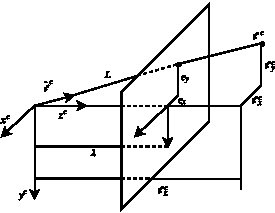
\includegraphics[width = 3.5in]{images/chapter2/camera_frame}
	\caption{Camera frame and visual aid for projective camera model}
	%
	\label{camera_frame}
\end{figure}

The camera frame, often called the optical frame, follows the common computer vision convention: $x$-axis is directed to the right, $y$-axis is directed down and the $z$-axis is directed out from the camera optical sensor (See Fig. \ref{camera_frame}). Thus, the rotation from the gimbal frame to the camera frame is fixed and is given by 
\begin{equation}
R^{c}_g =
\begin{bmatrix}
0 & 1 & 0 \\
0 & 0 & 1 \\
1 & 0 & 0
\end{bmatrix}.
\label{eq4}
\end{equation}

The basic idea of the projective camera model is that the 3D world is projected onto a 2D image plane that is orthogonal to $z^c$ axis with distance being the focal length $\lambda$ from the origin of the optical axis (See Fig. \ref{camera_frame}). Because of this projection, we lose the distance information to the target which introduces many problems in computer vision and estimation. 
The focal length of the camera is the distance between the optical sensor and the lens, and it can be obtained through camera calibration. Since common camera calibration gives the focal length in the units of pixels, the camera's field of view angle ($M$) can also be obtained as
\begin{equation}
M=2\tan^{-1}\bigg(\frac{\epsilon_{max}}{\lambda}\bigg)
\end{equation}
where $\epsilon_{max}$ is the maximum pixel value from the center of the image assuming the image is square. 

\subsection{Derivation}
Let the unit vector from the origin of the camera frame to the target (i.e. the line of sight vector or LOS vector) in the camera frame be defined as 
\begin{equation}
\hat{\ell}^c=\frac{1}{L}
\begin{pmatrix}
\epsilon_x \\
\epsilon_y \\
\lambda
\end{pmatrix}
=\frac{1}{\sqrt{\epsilon_x^2+\epsilon_y^2+\lambda^2}}
\begin{pmatrix}
\epsilon_x \\
\epsilon_y \\
\lambda
\end{pmatrix}
=\begin{pmatrix}
\hat{\ell}_x^c \\
\hat{\ell}_y^c \\
\hat{\ell}_z^c
\end{pmatrix}.
\label{unitlos}
\end{equation}
The angle commanding gimbal control algorithm computes the gimbal azimuth and elevation angles that would make the optical axis align with the unit LOS vector. By transforming the unit LOS vector (\ref{unitlos}) into the body frame, we get the desired optical axis as
\begin{equation}
\hat{\ell}^b=R_{g}^b R_{c}^g\hat{\ell}^c.
\label{unitbodylos}
\end{equation}
By equating the equation (\ref{unitbodylos}) to the unit optical axis vector transformed into the body frame, we can compute the desired azimuth and elevation commands as
\begin{align}
\hat{\ell}^b&=\begin{pmatrix}
\hat{\ell}_x^b \\
\hat{\ell}_y^b \\
\hat{\ell}_z^b
\end{pmatrix}=R_{g}^b(\alpha_{az}^d, \alpha_{el}^d) R_{c}^g\begin{pmatrix}
0 \\ 0 \\ 1
\end{pmatrix}
\\&=\begin{bmatrix}
\cos\alpha_{el}^d\cos\alpha_{az}^d & -\sin\alpha_{az}^d & \sin\alpha_{el}^d\cos\alpha_{az}^d \\
\cos\alpha_{el}^d\sin\alpha_{az}^d & \cos\alpha_{az}^d & \sin\alpha_{el}^d\sin\alpha_{az}^d \\
-\sin\alpha_{el}^d & 0 & \cos\alpha_{el}^d
\end{bmatrix}
\begin{bmatrix}
0 & 0 & 1 \\
1 & 0 & 0 \\
0 & 1 & 0
\end{bmatrix}
\begin{pmatrix}
0 \\ 0 \\ 1
\end{pmatrix}
\\&=\begin{pmatrix}
\cos\alpha_{el}^d\cos\alpha_{az}^d \\
\cos\alpha_{el}^d\sin\alpha_{az}^d \\
-\sin\alpha_{el}^d
\end{pmatrix}.
\end{align}
Solving for $\alpha_{az}^d$ and $\alpha_{el}^d$ as 
\begin{equation}
\alpha_{az}^d=\tan^{-1}
\begin{pmatrix}
\frac{\hat{\ell}_y^b}{\hat{\ell}_x^b}
\end{pmatrix}
\end{equation}
\begin{equation}
\alpha_{el}^d=-\sin^{-1}
\begin{pmatrix}
\hat{\ell}_z^b
\end{pmatrix},
\end{equation}
results in the gimbal commands that place the object of interest at the center of the image.

\subsection{Hardware Result}
\begin{figure}[htbp]
	\centering
	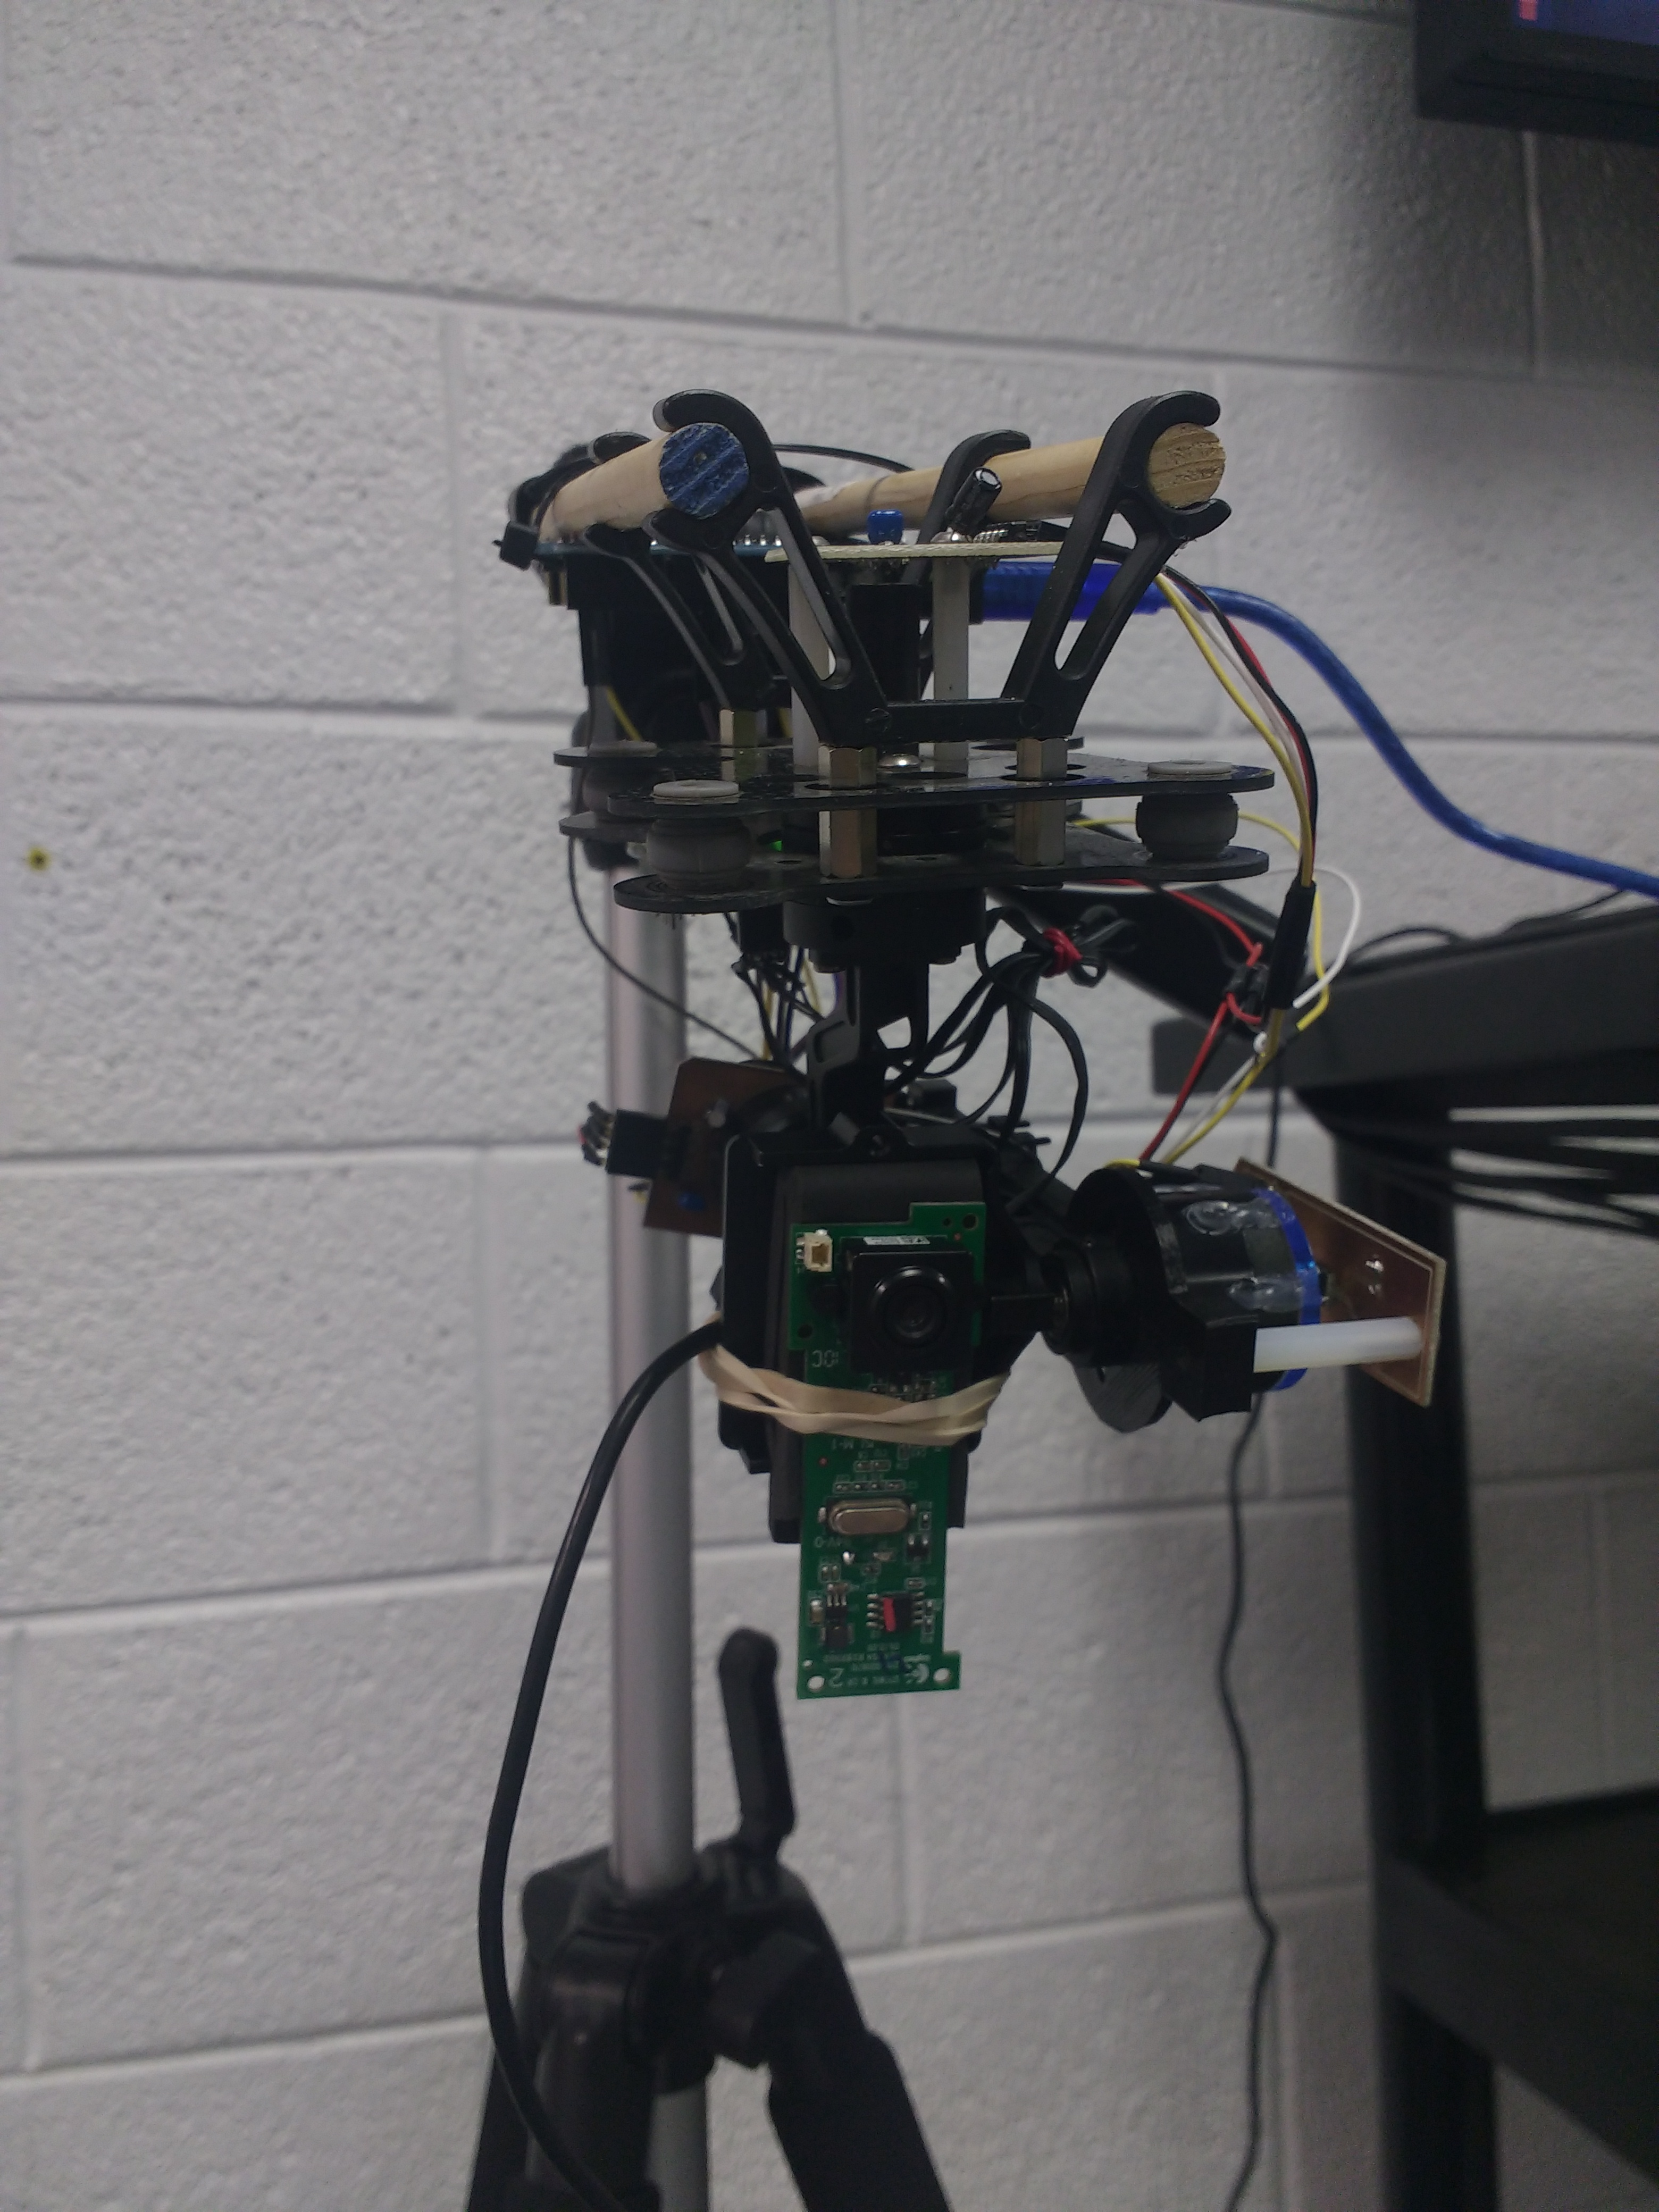
\includegraphics[width = 3in]{images/chapter2/gimbal_webcam.jpg}
	\caption{Prototype hardware to test the gimbal control algorithm}
	\label{gimbal_webcam}
\end{figure}

The gimbal control algorithm has been implemented and tested with simple hardware (see Figure \ref{gimbal_webcam}). The major hardware component includes the BaseCam SimpleBGC 32-bit gimbal controller, a webcam, DYS 3-axis GoPro gimbal, and the AS5048B magnetic rotary encoder attached to each rotating axis to measure the gimbal angles. Note that in this hardware experiment, the roll axis of the gimbal is always commanded to be zero to model a pan-tilt gimbal. The focal length of the camera is known through the camera calibration process and the target pixel location is given by the color detection algorithm implemented in OpenCV \cite{itseez2015opencv}. The objective of the gimbal control is to keep the target at the center of the camera field of view (see Figure \ref{gimbal_result}. A video of the results can be found at \href{https://www.youtube.com/watch?v=OZ0Mg8AoAzk}{https://www.youtube.com/watch?v=OZ0Mg8AoAzk}). 

\begin{figure*}[htbp]
	\centering
	\begin{subfigure}{0.5\textwidth}
		\centering
		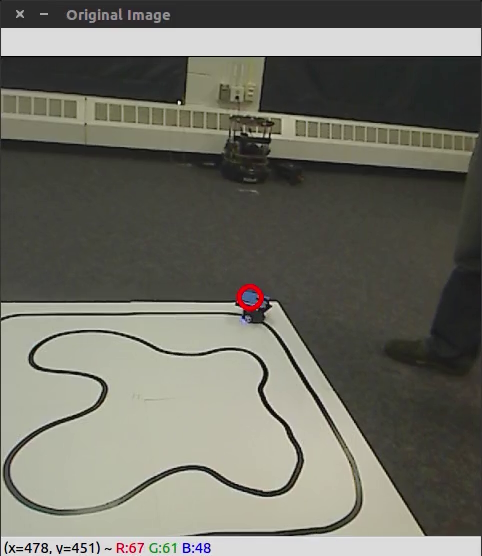
\includegraphics[height=6cm]{images/chapter2/gimbal_0s.png}
		\caption{when $t=0s$}
	\end{subfigure}%
	\begin{subfigure}{0.5\textwidth}
		\centering
		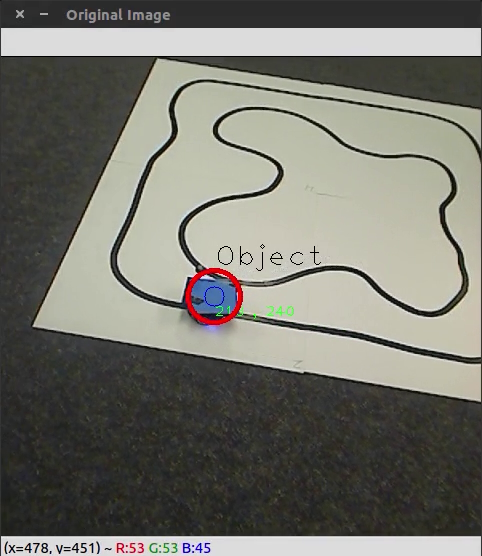
\includegraphics[height=6cm]{images/chapter2/gimbal_10s.png}
		\caption{when $t=10s$}
	\end{subfigure}
	\begin{subfigure}{0.5\textwidth}
		\centering
		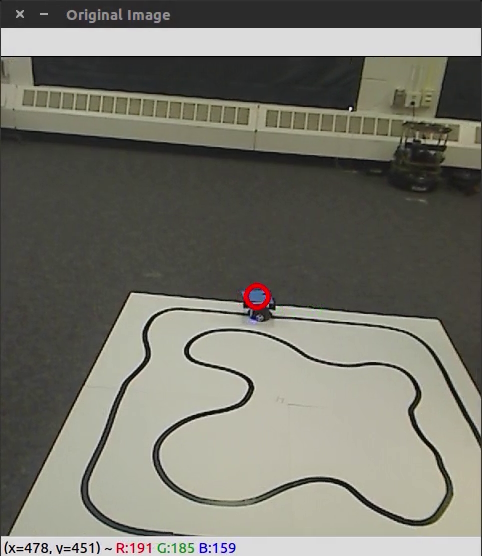
\includegraphics[height=6cm]{images/chapter2/gimbal_20s.png}
		\caption{when $t=20s$}
	\end{subfigure}%
	\begin{subfigure}{0.5\textwidth}
		\centering
		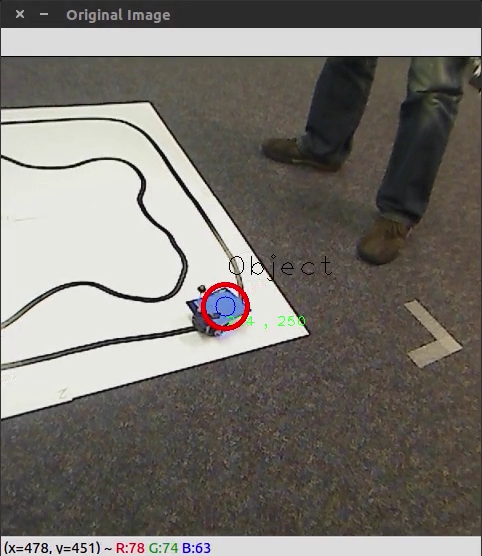
\includegraphics[height=6cm]{images/chapter2/gimbal_30s.png}
		\caption{when $t=30s$}
	\end{subfigure}
	\begin{subfigure}{0.5\textwidth}
		\centering
		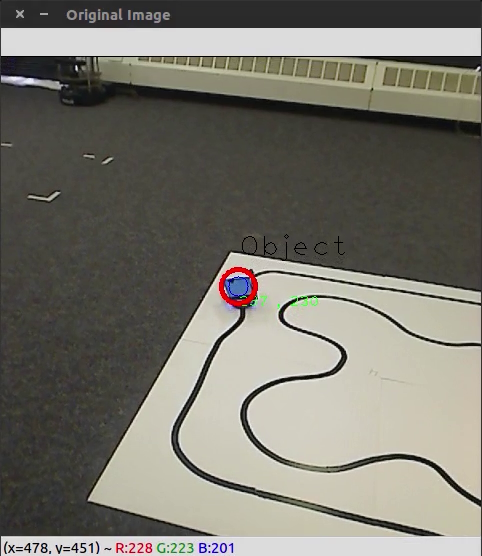
\includegraphics[height=6cm]{images/chapter2/gimbal_40s.png}
		\caption{when $t=40s$}
	\end{subfigure}	
	\caption{Hardware demonstration. The gimbal control algorithm is keeping the target object at the center of the camera field of view.}
	\label{gimbal_result}
\end{figure*}


\section{Angular Velocity Commanding Gimbal Control}
In the previous section, a relatively simple gimbal control algorithm is presented. One disadvantage of that algorithm is that it does not take the camera velocity into consideration. When the gimbal is mounted on a stationary platform, the angle commanding controller can perform without any performance degradation. However, if the gimbal is mounted on a moving UAV, then taking the camera velocity into account in the controller becomes important. The work in \cite{Hurak2012} addresses this issue and derives an algorithm that overcomes the issue. This angular velocity commanding gimbal control algorithm is presented briefly in this section because some of the concepts in this section introduces important background for the next section. 

\begin{figure}[htbp]
	\centering
	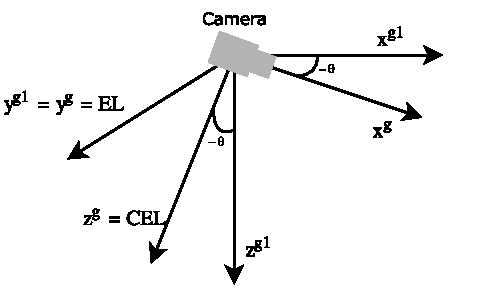
\includegraphics[width = 3in]{images/chapter2/cross_elevation.pdf}
	\caption{Elevation and cross-elevation axis}
	\label{cross_elevation}
\end{figure}
\subsection{Image Jacobian}
A full derivation of getting Image Jacobian matrix (often called interaction matrix) can be found in \cite{spong2006robot}. Here, we only show the final form of the Image Jacobian in the process of developing the gimbal control algorithm. Let the camera translational and rotational velocities both expressed in the camera frame be defined as
\begin{equation}
\mathbf{v}^c=[v_x^c, v_y^c, v_z^c]^\top
\end{equation}
\begin{equation}
\mathbf{\omega}^c=[\omega_x^c, \omega_y^c, \omega_z^c]^\top
\end{equation}
\begin{equation}
\mathbf{\xi}=[{\mathbf{v}^c}^\top, {\mathbf{\omega}^c}^\top]^\top.
\label{camera_velocity}
\end{equation}
Let $\alpha_{el}$ be the elevation angle, and let $\alpha_{az}$ be the azimuth angle. Also, following the convention in Figure \ref{camera_frame}, 
\begin{equation}
R^{g}_c =
\begin{bmatrix}
0 & 0 & 1 \\
1 & 0 & 0 \\
0 & 1 & 0
\end{bmatrix}.
\end{equation}
Also, let the coordinates of an image feature and its pixel velocity be defined as 
\begin{equation}
\mathbf{s}=[u, w]^\top
\end{equation}
and 
\begin{equation}
\mathbf{\dot{s}}=[\dot{u}, \dot{w}]^\top.
\label{image_feature_velocity}
\end{equation}
The Image Jacobian matrix $L$ at $\mathbf{s}$ is the relationship between the camera velocity in (\ref{camera_velocity}) and the image feature velocity in (\ref{image_feature_velocity}) and can be expressed as 
\begin{equation}
\mathbf{\dot{s}}=L(\mathbf{s},z,\lambda)\mathbf{\xi}
\end{equation}
or more explicitly
\begin{equation}
\begin{bmatrix}
\dot{u} \\ \dot{w}
\end{bmatrix}
=\begin{bmatrix}
-\frac{\lambda}{z} & 0 & \frac{u}{z} & \frac{uw}{\lambda} & -\frac{\lambda^2+u^2}{\lambda} & w \\
0 & -\frac{\lambda}{z} & \frac{w}{z} & \frac{\lambda^2+w^2}{\lambda} & -\frac{uw}{\lambda} & -u
\end{bmatrix}
\begin{bmatrix}
v_x^c \\ v_y^c \\ v_z^c \\
\omega_x^c \\ \omega_y^c \\ \omega_z^c
\end{bmatrix}
\label{image_jacobian}
\end{equation}
where $z$ is the depth along the optical axis to the target, and $\lambda$ is the focal length. Note that $\lambda$ is a fixed parameter once the camera is calibrated. The equation (\ref{image_jacobian}) can be divided into two parts: one for the camera translational velocity and the other for rotational velocity as
\begin{align}
\mathbf{\dot{s}}&=\begin{bmatrix}
-\frac{\lambda}{z} & 0 & \frac{u}{z} \\
0 & -\frac{\lambda}{z} & \frac{w}{z}
\end{bmatrix}\mathbf{v}^c+
\begin{bmatrix}
\frac{uw}{\lambda} & -\frac{\lambda^2+u^2}{\lambda} & w \\
\frac{\lambda^2+w^2}{\lambda} & -\frac{uw}{\lambda} & -u
\end{bmatrix}\mathbf{\omega}^c
\\&=L_v(u,w,z)\mathbf{v}^c+L_{\omega}(u,w)\mathbf{\omega}^c
\label{image_jacobian1}
\end{align}
It is worth noting that only the translational term depends on the target depth $z$. 

\subsection{Feedback Linearization-based Visual Pointing and Tracking}
The control objective is to drive an image feature to the center of the image. The horizontal error can be eliminated by moving two axis gimbal motors attached on azimuth and elevation axis. Moving only the azimuth axis cannot fully compensate for the horizontal error because it only indirectly affects $z^g$ axis which is often referred as cross-elevation axis $cel$ (see Figure \ref{cross_elevation}). Thus, some vertical error is introduced and it needs to be compensated by moving the elevation at next time step. However, the key idea of the controller is that by exploiting $\omega_x^g$ term which is the angular velocity along the optical axis, we can find the azimuth and elevation commands for the same time step that smoothly compensates for the horizontal error without introducing the vertical error. Let the error in the image plane be
\begin{equation}
e(t)=s(t)-s^{ref}
\label{image_feature_error}
\end{equation}
where $s^{ref}=[0, 0]^\top$ to push the image feature to the image center. We would like to drive $e(t)$ to zeros by controlling the elevation angular velocity $\omega_{EL}=\omega_y^g$ and the azimuth angular velocity $\omega_{az}=\frac{\omega_z^g}{\cos \alpha_{el}}$. Re-arranging equation (\ref{image_jacobian1}) gives
\begin{equation}
L_{\omega}(u,w)\mathbf{\omega}^c=\dot{s}-L_v(u,w,z)\mathbf{v}^c.
\label{image_jacobian2}
\end{equation}
Note that we can only command the camera angular rate where the camera linear velocity can be measured by other sensors. The null space of the matrix $L_{\omega}$ can be parameterized as
\begin{equation}
\mathcal{N}\{L_{\omega}\}=\{k\begin{bmatrix}
u & w & \lambda
\end{bmatrix}^\top\}.
\label{nullspace}
\end{equation}
Therefore adding (\ref{nullspace}) to (\ref{image_jacobian2}) gives
\begin{equation}
L_{\omega}(u,w)\mathbf{\omega}^c=\dot{s}-L_v(u,w,z)\mathbf{v}^c+L_{\omega}(u,w)k\begin{bmatrix}
u \\ w \\ \lambda
\end{bmatrix}.
\label{image_jacobian3}
\end{equation}
The null space parametrization means that a rotation about the axis connecting the image feature and the origin of the optical axis does not change the coordinates of the image feature. The left pseudoinverse of $L_{\omega}$ is given by 
\begin{equation}
L_{\omega}^\sharp=\begin{bmatrix}
0 & \frac{\lambda}{\lambda^2+u^2+w^2} \\
-\frac{\lambda}{\lambda^2+u^2+w^2} & 0 \\
\frac{w}{\lambda^2+u^2+w^2} & -\frac{u}{\lambda^2+u^2+w^2}
\end{bmatrix}.
\label{pseudoinverse}
\end{equation}
Multiplying both side of (\ref{image_jacobian3}) by (\ref{pseudoinverse}) yields
\begin{equation}
\mathbf{\omega}^c=\frac{1}{z(\lambda^2+u^2+w^2)}\begin{bmatrix}
\lambda^2 v_y-\lambda v_z w+\lambda \dot{w}z+ku \\
-\lambda^2 v_x+\lambda v_zu-\lambda \dot{u}z+kw \\
-\lambda u v_y+\lambda w v_x-u\dot{w}z+\dot{u}wz+k\lambda
\end{bmatrix}.
\label{angular_rate}
\end{equation}
If we require $\dot{s}^{ref}(t)=-\alpha Is(t)$ where $\alpha$ is a positive value, the actual value of $s(t)$ is expected to be exponentially stable which means it converges to zero. Thus, 
\begin{equation}
\mathbf{\dot{s}}^{ref}=\begin{bmatrix}
\dot{u}^{ref} \\ \dot{w}^{ref}
\end{bmatrix}
=-\alpha \begin{bmatrix}
1 & 0 \\ 0 & 1
\end{bmatrix}
\begin{bmatrix}
u \\ w
\end{bmatrix}
=\begin{bmatrix}
-\alpha u \\ -\alpha w
\end{bmatrix}.
\label{sdot_reference}
\end{equation}
By plugging equation (\ref{sdot_reference}) into (\ref{angular_rate}), we can compute the desired camera angular rate that guarantees the asymptotic stability for the image error as
\begin{equation}
{\mathbf{\omega}^c}^{ref}=\frac{1}{z(\lambda^2+u^2+w^2)}\begin{bmatrix}
\lambda^2 v_y-\lambda v_z w -\lambda \alpha wz+ku \\
-\lambda^2 v_x+\lambda v_zu +\lambda \alpha uz+kw \\
-\lambda u v_y+\lambda w v_x +k\lambda
\end{bmatrix}.
\label{angular_rate_reference}
\end{equation}
This angular rate reference command expressed in the camera frame must be transformed into the gimbal frame in order to command each gimbal axis as
\begin{align}
{\mathbf{\omega}^g}^{ref}&=R_c^g{\mathbf{\omega}^c}^{ref}
=\begin{bmatrix}
{\omega_x^g}^{ref} \\ {\omega_y^g}^{ref} \\ {\omega_z^g}^{ref}
\end{bmatrix}
\\&=\frac{1}{z(\lambda^2+u^2+w^2)}\begin{bmatrix}
-\lambda u v_y+\lambda w v_x +k\lambda \\
\lambda^2 v_y-\lambda v_z w -\lambda \alpha wz+ku \\
-\lambda^2 v_x+\lambda v_zu +\lambda \alpha uz+kw \\
\end{bmatrix}.
\label{angular_rate_ref_elevation}
\end{align}
Unfortunately ${\mathbf{\omega}^c}^{ref}$ contains reference commands for three axes, but there are only two controllable axes, namely azimuth and elevation. This problem can be solved by using the free parameter $k$ to come up with two proper motor commands. The key strategy is to select $k$ so that $\omega_x^g=0$. Accordingly,  
\begin{equation}
k=uv_y-wv_x+\frac{z(\lambda^2+u^2+w^2)}{\lambda}\omega_x^g
\label{k}
\end{equation}
where $\omega_x^g$ must be measured from a sensor such as a MEMS gyro attached to the camera. Substituting for $k$ in ${\omega_y^g}^{ref}$ and ${\omega_z^g}^{ref}$ from the equation (\ref{angular_rate_ref_elevation}) with (\ref{k}) gives
\begin{equation}
\omega_{el}^{ref}={\omega_y^g}^{ref}=\frac{\lambda^2 v_y-\lambda v_z w -\lambda \alpha wz+u^2 v_y-uwv_x}{z(\lambda^2+u^2+w^2)}+\frac{\omega_x^g u}{\lambda}
\end{equation}
\begin{equation}
\omega_{cel}^{ref}={\omega_z^g}^{ref}=\frac{-\lambda^2 v_x+\lambda v_z u+\lambda \alpha uz +uwv_y -w^2 v_x}{z(\lambda^2+u^2+w^2)}+\frac{\omega_x^g w}{\lambda}.
\end{equation}
Using the relationship 
\begin{equation}
\omega_{az}=\frac{1}{\cos\alpha_{el}}\omega_{cel},
\end{equation}
we can compute the desired angular rate on the azimuth axis as
\begin{equation}
\omega_{az}^{ref}=\frac{1}{\cos \alpha_{el}}\bigg(\frac{-\lambda^2 v_x+\lambda v_z u+\lambda \alpha uz +uwv_y -w^2 v_x}{z(\lambda^2+u^2+w^2)}+\frac{\omega_x^g w}{\lambda}\bigg).
\end{equation}
\begin{figure}[htbp]
	\centering
	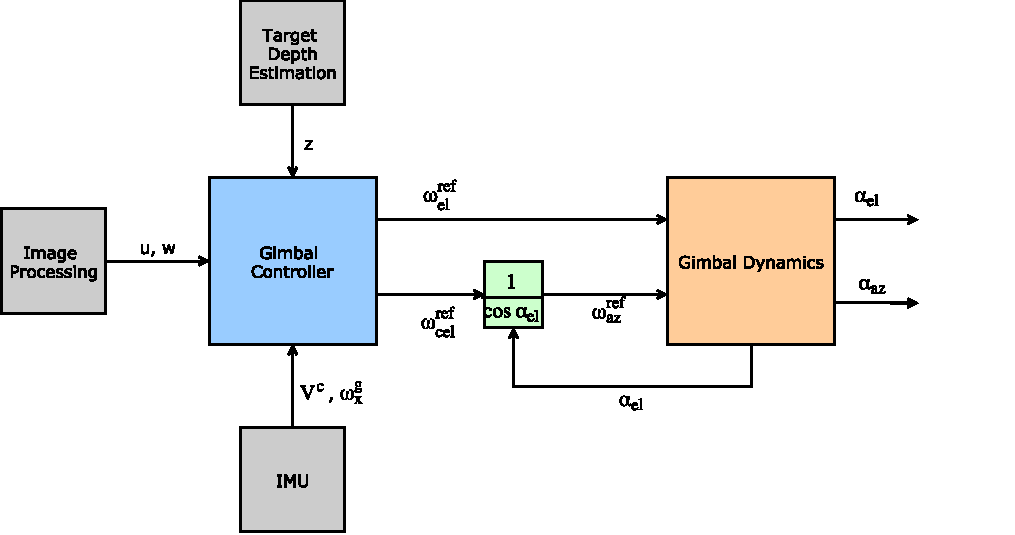
\includegraphics[width = 5in]{images/chapter2/gp_blockdiagram.pdf}
	\caption{Angular velocity commanding gimbal controller block diagram}
	\label{avcg_blockdiagram}
\end{figure}
The system block diagram of this controller is shown in Figure \ref{avcg_blockdiagram}. The controller presents the ideal control scheme for a two axis inertially stabilized gimbal system, but it also presents some technical challenges such as estimating the depth to the target or estimating the camera translational velocity. The camera translational velocity can be either estimated by using the UAV velocity if available or be treated as a disturbance. Estimating the depth can be handled using a laser range finder if available or geolocation technique. Another option is to use the novel adaptive depth gimbal control algorithm that we introduce in the next section.

\section{Adaptive Depth Gimbal Control}
The gimbal control algorithm in the previous section provides a method to keep a target of interest in the camera's field of view with gimbal azimuth and elevation control. However, the target depth $z$ is required to complete the Jacobian (\ref{image_jacobian}). This section examines a strategy to remove this requirement by estimating the depth online. This controller is derived using Model Reference Adaptive Control (MRAC).

\subsection{Introduction}
Model Reference Adaptive Control (MRAC) is a useful control scheme to stabilize dynamical systems even when there are unknown parameters in the system. A general MRAC closed-loop block diagram can be found in Figure \ref{MRAC_blockdiagram} \cite{Lavretsky2013}. The design of an MRAC system requires a reference model that specifies how the actual system should behave. An adaptive law then adapts the parameters using the error between the reference model and the system output. Finally, the controller computes the command for the plant using the adjusted parameters, the external command, and the system output. 
\begin{figure}[htbp]
	\centering
	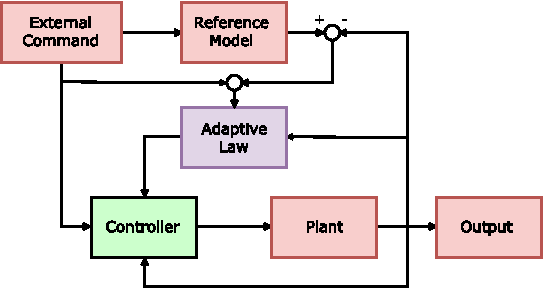
\includegraphics[width = 5in]{images/chapter2/MRAC.pdf}
	\caption{An MRAC closed-loop block diagram}
	\label{MRAC_blockdiagram}
\end{figure}
\subsection{Derivation}
Consider again the Image Jacobian matrix
\begin{equation}
\begin{bmatrix}
\dot{u} \\ \dot{w}
\end{bmatrix}
=\begin{bmatrix}
-\frac{\lambda}{z} & 0 & \frac{u}{z} & \frac{uw}{\lambda} & -\frac{\lambda^2+u^2}{\lambda} & w \\
0 & -\frac{\lambda}{z} & \frac{w}{z} & \frac{\lambda^2+w^2}{\lambda} & -\frac{uw}{\lambda} & -u
\end{bmatrix}
\begin{bmatrix}
v_x^c \\ v_y^c \\ v_z^c \\
\omega_x^c \\ \omega_y^c \\ \omega_z^c
\end{bmatrix}\\
\label{image_jacobian4}
\end{equation}
or for simplicity
\begin{equation}
\mathbf{\dot{s}}=L_v(u,w,z)\mathbf{v}^c+L_{\omega}(u,w)\mathbf{\omega}^c.
\end{equation}
Since we desire that the target is pushed to the center of the image plane, the reference model can be set as 
\begin{equation}
\mathbf{\dot{s}}^{ref}=A\mathbf{s}^{ref}
\label{reference_model}
\end{equation}
where $\mathbf{s}=[u, w]^\top$ and $A$ is Hurwitz (i.e. every eigenvalue of $A$ has strictly negative real part). It is clear that the reference model in (\ref{reference_model}) is globally asymptotically stable. From the image jacobian matrix, $\mathbf{\omega}^c$ is the control input, because it is common situation to track the target with gimbal movement rather than platform movement. Thus, equation (\ref{image_jacobian4}) can be manipulated into a more convenient form for MRAC design as 
\begin{align}
\mathbf{\dot{s}}
&=\frac{1}{z}
\begin{bmatrix}
-\lambda v_x^c+uv_z^c \\
-\lambda v_y^c+wv_z^c \\
\end{bmatrix}
+\begin{bmatrix}
\frac{uw}{\lambda} & -\frac{\lambda^2+u^2}{\lambda} & w \\
\frac{\lambda^2+w^2}{\lambda} & -\frac{uw}{\lambda} & -u
\end{bmatrix}
\begin{bmatrix}
\omega_x^c \\ \omega_y^c \\ \omega_z^c
\end{bmatrix}
\\&=\beta\varphi + L_{\omega}U
\label{adaptive_image_jacobian}
\end{align}
where $U$ is the control input and $\beta=\frac{1}{z}$. If $\beta$ were known, then the ideal control input would be
\begin{equation}
U=L_\omega^\sharp(-\beta\varphi+K\mathbf{s})
\end{equation}
where $L_\omega^\sharp$ is the right pseudoinverse of $L_\omega$ and $K$ is a negative definite tuning matrix. Then, the subsequent dynamics would become
\begin{equation}
\mathbf{\dot{s}}=K\mathbf{s}
\end{equation}
which is globally asymptotically stable. However, since $\beta$ is an unknown quantity and needs to be adapted, a more realistic control input is
\begin{equation}
U=L_\omega^\sharp(-\hat{\beta}\varphi+K\mathbf{s})
\end{equation}
where $\hat{\beta}$ is the estimate of $\beta$. Plugging this control input into the equation (\ref{adaptive_image_jacobian}) gives
\begin{align}
\mathbf{\dot{s}}&=\beta\varphi-\hat{\beta}\varphi+K\mathbf{s}
\\&= \tilde{\beta}\varphi+K\mathbf{s}
\end{align}
where $\tilde{\beta}=\beta-\hat{\beta}$. Let the error be defined as 
\begin{equation}
\mathbf{e}=\mathbf{s}-\mathbf{s}^{ref}.
\end{equation}
Taking derivative and equating $K$ to $A$ gives
\begin{align}
\dot{\mathbf{e}}&=\dot{\mathbf{s}}-\dot{\mathbf{s}}^{ref}
\\&=\tilde{\beta}\varphi+K\mathbf{s}-A\mathbf{s}^{ref}
\\&=\tilde{\beta}\varphi+A\mathbf{e}.
\end{align}
Using the variables of interest, a Lyapunov function candidate can be constructed as 
\begin{equation}
V=\frac{1}{2}\mathbf{e}^\top\mathbf{e}+\frac{1}{2\gamma_\beta}\tilde{\beta}^2.
\end{equation}
Taking the derivative yields
\begin{align}
\dot{V}&=\mathbf{e}^\top\dot{\mathbf{e}}+\frac{1}{\gamma_\beta}\tilde{\beta}\dot{\tilde{\beta}}
\\&=\mathbf{e}^\top(\tilde{\beta}\varphi+A\mathbf{e})+\frac{1}{\gamma_\beta}\tilde{\beta}\dot{\tilde{\beta}}.
\label{vdot2}
\end{align}
Assuming that the inverse depth $\beta$ is constant or slowly moving ($\dot{\beta}=0$, $\dot{\tilde{\beta}}=-\dot{\hat{\beta}}$), the above equation becomes
\begin{align}
\dot{V}&=\mathbf{e}^\top A\mathbf{e}+\tilde{\beta}(\mathbf{e}^\top\varphi-\frac{\dot{\hat{\beta}}}{\gamma_\beta}).
\end{align}
Since $\dot{\hat{\beta}}$ is a design parameter, its value can be selected as 
\begin{equation}
\dot{\hat{\beta}}=\gamma_\beta\mathbf{e}^\top\varphi.
\end{equation}
Then, the equation (\ref{vdot2}) becomes
\begin{equation}
\dot{V}=\mathbf{e}^\top A\mathbf{e}.
\end{equation}
Asymptotic stability of the system follows from the fact that A is Hurwitz.
\subsection{Simulation}
First, the reference model $\mathbf{s}^{ref}$, in equation (\ref{reference_model}) is selected as $[0, 0]$ over time. The objective of the MRAC controller is to drive the actual image dynamics with unknown quantity $z$ as close as it can to the reference model. In simulation, a square image with 800 pixel width and height is used. The camera field of view is set to 60 degrees and one pixel is set to one millimeter. Thus, we can obtain the focal length and image width in metric units. The initial image coordinates are randomly selected and these coordinates are expected to converge to the origin as the reference model. In reality, the depth $z$ is a varying quantity because of the relative movement between the camera and the target. However, in this simulation $z$ is initialized to an arbitrary value between 30 and 300, and is changed randomly with increment $\pm2$ every second. In order to simulate the translational velocity of the UAV, $v_x^c$ and $v_y^c$ are initialized to zeros and changed with increment $\pm2$ every other second. $v_z^c$ is kept zero assuming that the camera is not directly flying into nor away from the target. Figure \ref{adaptive_result} shows that the controller keeps the target in the center of the image which is the primary objective. Figure \ref{adaptive_command} presents the angular velocity commands computed by the adaptive depth gimbal controller and the depth estimation. Based on Figure \ref{adaptive_command}, the estimation of the uncertain parameter seems to converge to its true value. However, note that this is rather a special case. In normal cases, only uniform boundness of the uncertain parameters is guaranteed \cite{Lavretsky2013}. 
\begin{figure*}[htbp]
	\centering
	\begin{subfigure}{0.5\textwidth}
		\centering
		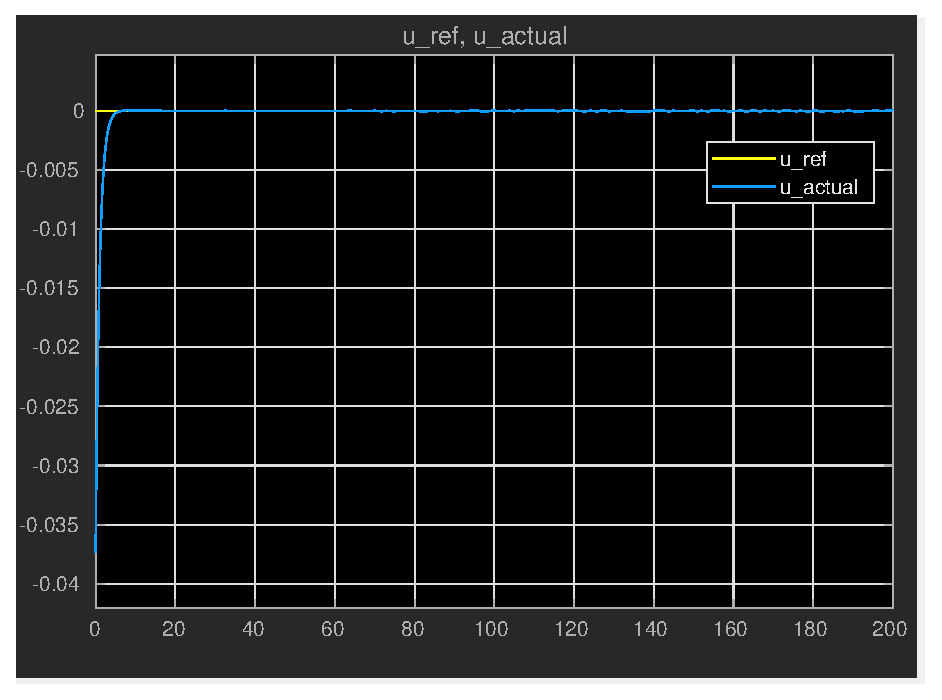
\includegraphics[width=0.9\linewidth]{images/chapter2/u_adaptive}
		\caption{Reference image coordinate $u_{ref}$ and the system output $u$}
	\end{subfigure}%
	\begin{subfigure}{0.5\textwidth}
		\centering
		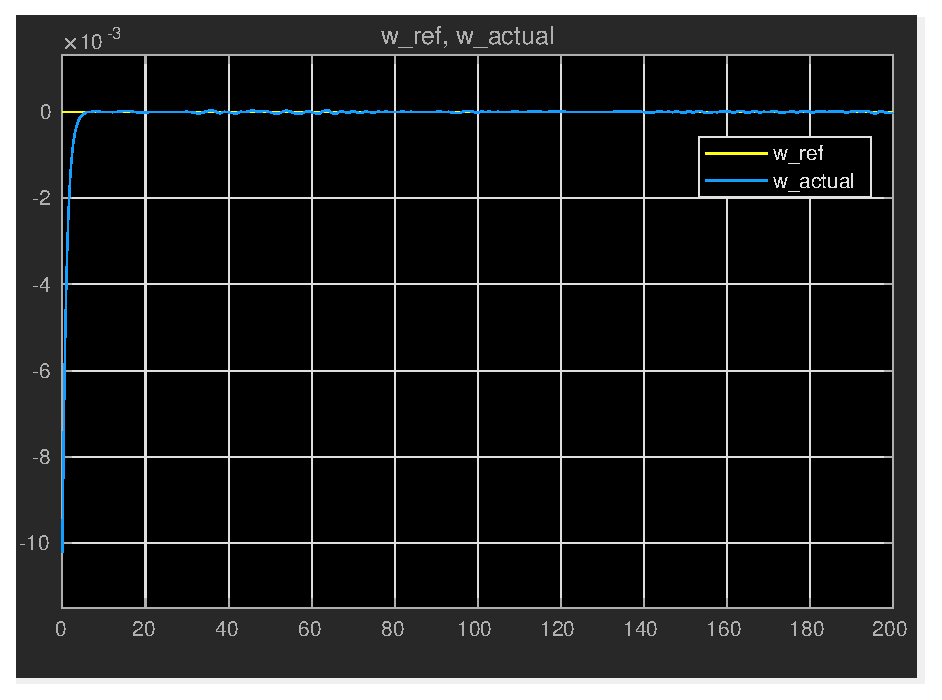
\includegraphics[width=0.9\linewidth]{images/chapter2/w_adaptive}
		\caption{Reference image coordinate $w_{ref}$ and the system output $w$}
	\end{subfigure}
	\caption{The simulation result for the adaptive depth gimbal control. The system output $u$ and $w$ are converging to the reference model output $u_{ref}$ and $w_{ref}$.}
	\label{adaptive_result}
\end{figure*}

\begin{figure*}[htbp]
	\centering
	\begin{subfigure}{0.5\textwidth}
		\centering
		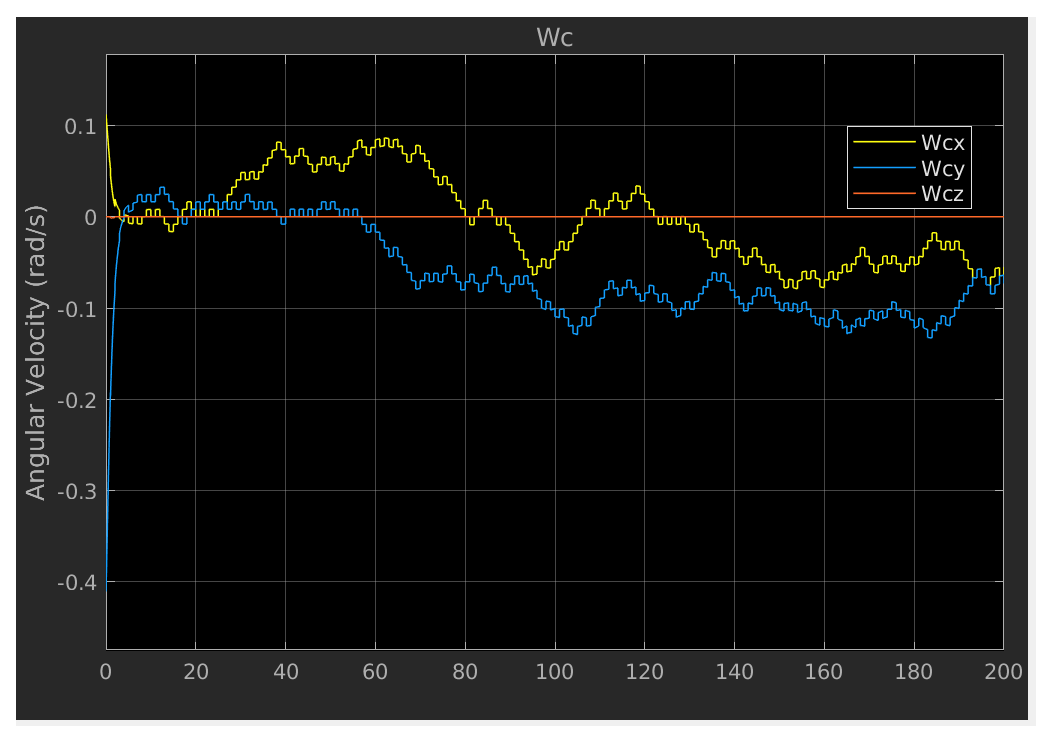
\includegraphics[width=0.9\linewidth]{images/chapter2/angular_velocity_adaptive}
		\caption{Angular velocity commands of the controller}
	\end{subfigure}%
	\begin{subfigure}{0.5\textwidth}
		\centering
		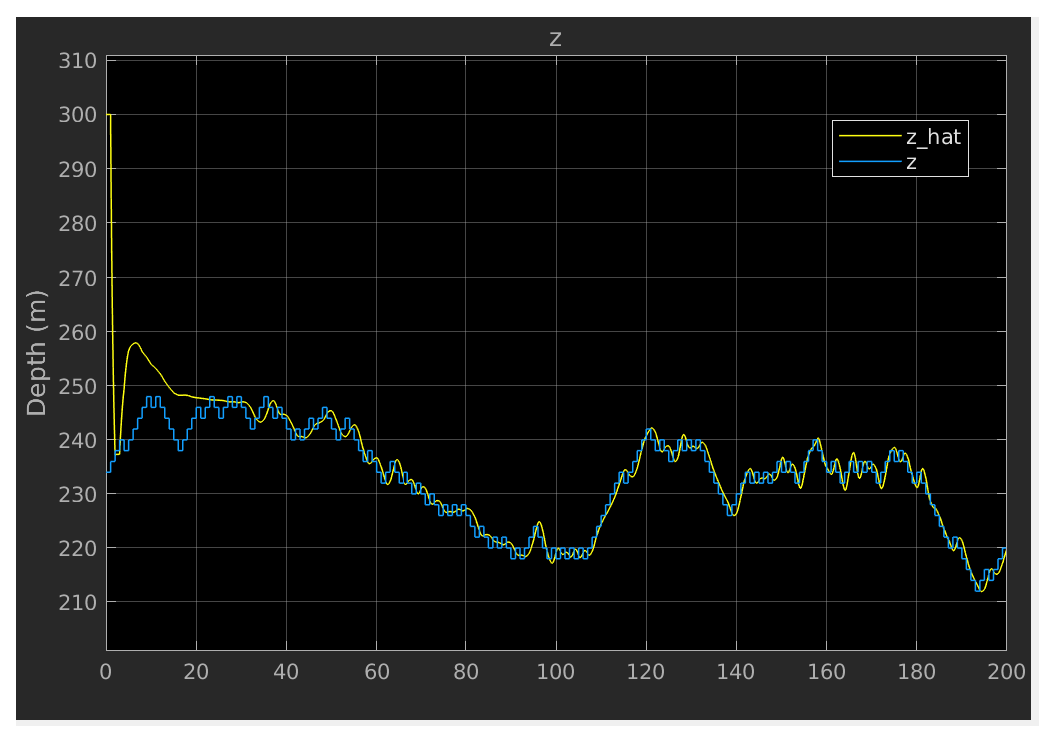
\includegraphics[width=0.9\linewidth]{images/chapter2/z_adaptive}
		\caption{Online depth estimation, $\hat{z}$}
	\end{subfigure}
	\caption{Angular velocity commands of the adaptive depth gimbal controller. Note that only two commands are used, since it is a pan-tilt gimbal. The depth $z$ estimate using MRAC.}
	\label{adaptive_command}
\end{figure*}

In addition, this gimbal control is simulated on a multirotor equipped with a pan-tilt gimbal. The multirotor is moving and suppose that its translational velocity is available. Also, the target is moving on the ground. The adaptive depth gimbal controller takes the pixel location of the target from a camera at a $30Hz$ frame rate, and its goal is to push the target to the center of the image. The simulated multirotor and camera view are presented in Figure \ref{uav_adaptive}. Additional information regarding the simulation can be found in Figure \ref{uav_adaptive_additional}. These plots are rather typical for MRAC: meeting the control objective without a guarantee that the uncertain parameter will converge to its true value. 

\begin{figure*}[htbp]
	\centering
	\begin{subfigure}{0.5\textwidth}
		\centering
		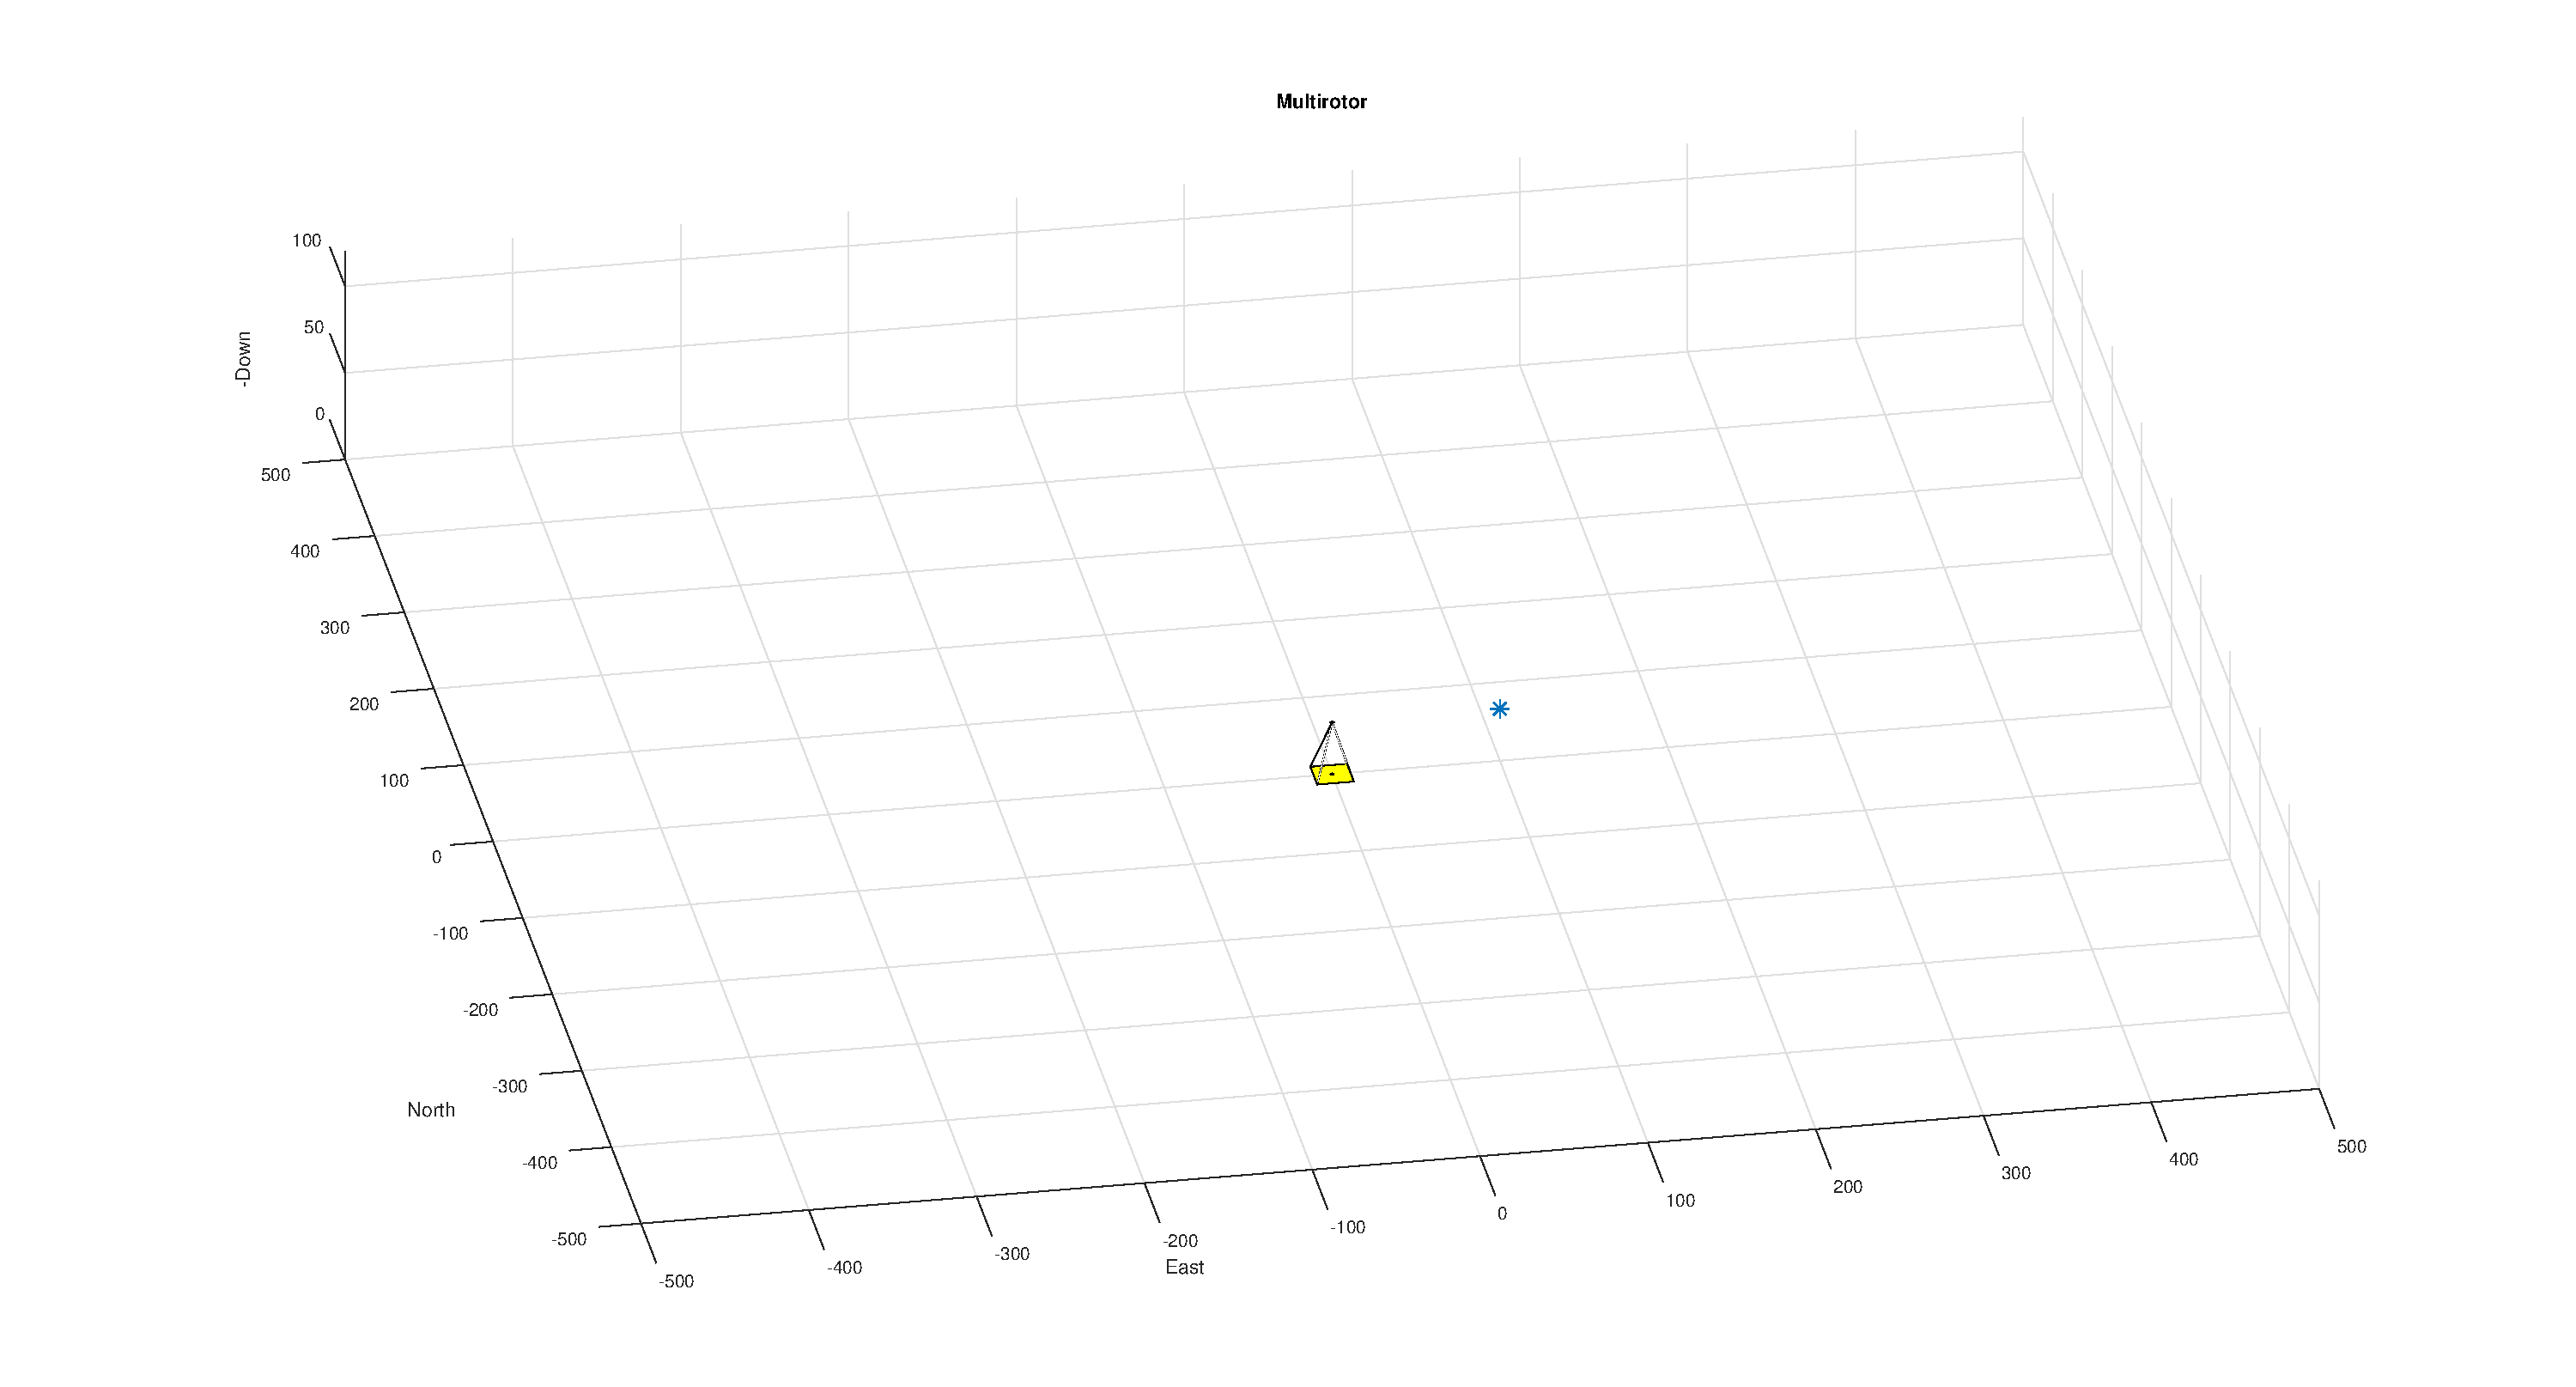
\includegraphics[height=4.5cm]{images/chapter2/uav_adaptive_0s}
		\caption{Multirotor at $t=0s$. The blue star indicates the desired multirotor position for the position PID controller for moving camera platform.}
	\end{subfigure}%
	\begin{subfigure}{0.5\textwidth}
		\centering
		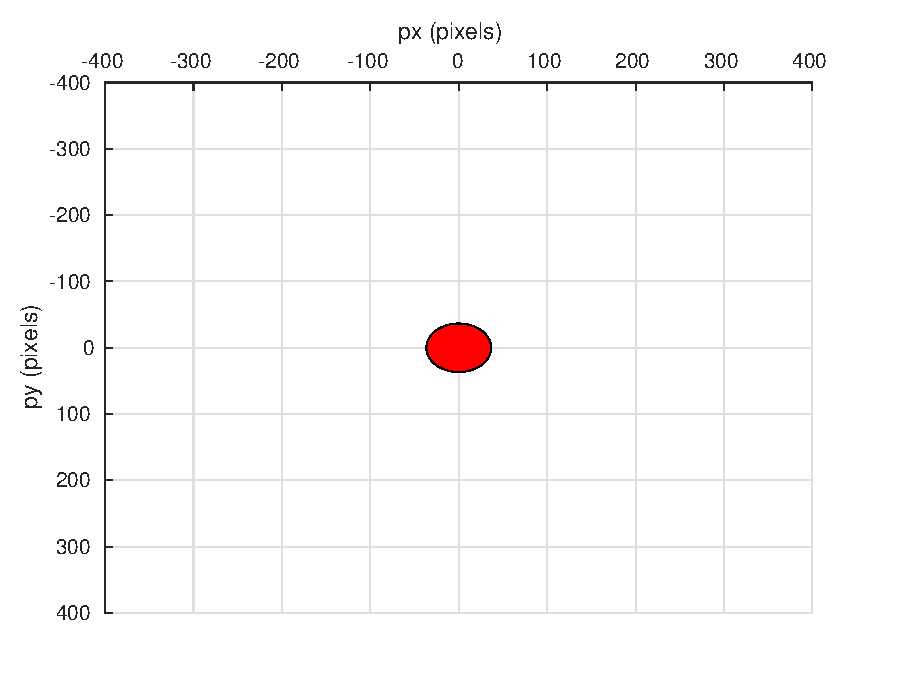
\includegraphics[height=4.5cm]{images/chapter2/camera_adaptive_0s}
		\caption{Camera view at $t=0s$}
	\end{subfigure}
	\begin{subfigure}{0.5\textwidth}
		\centering
		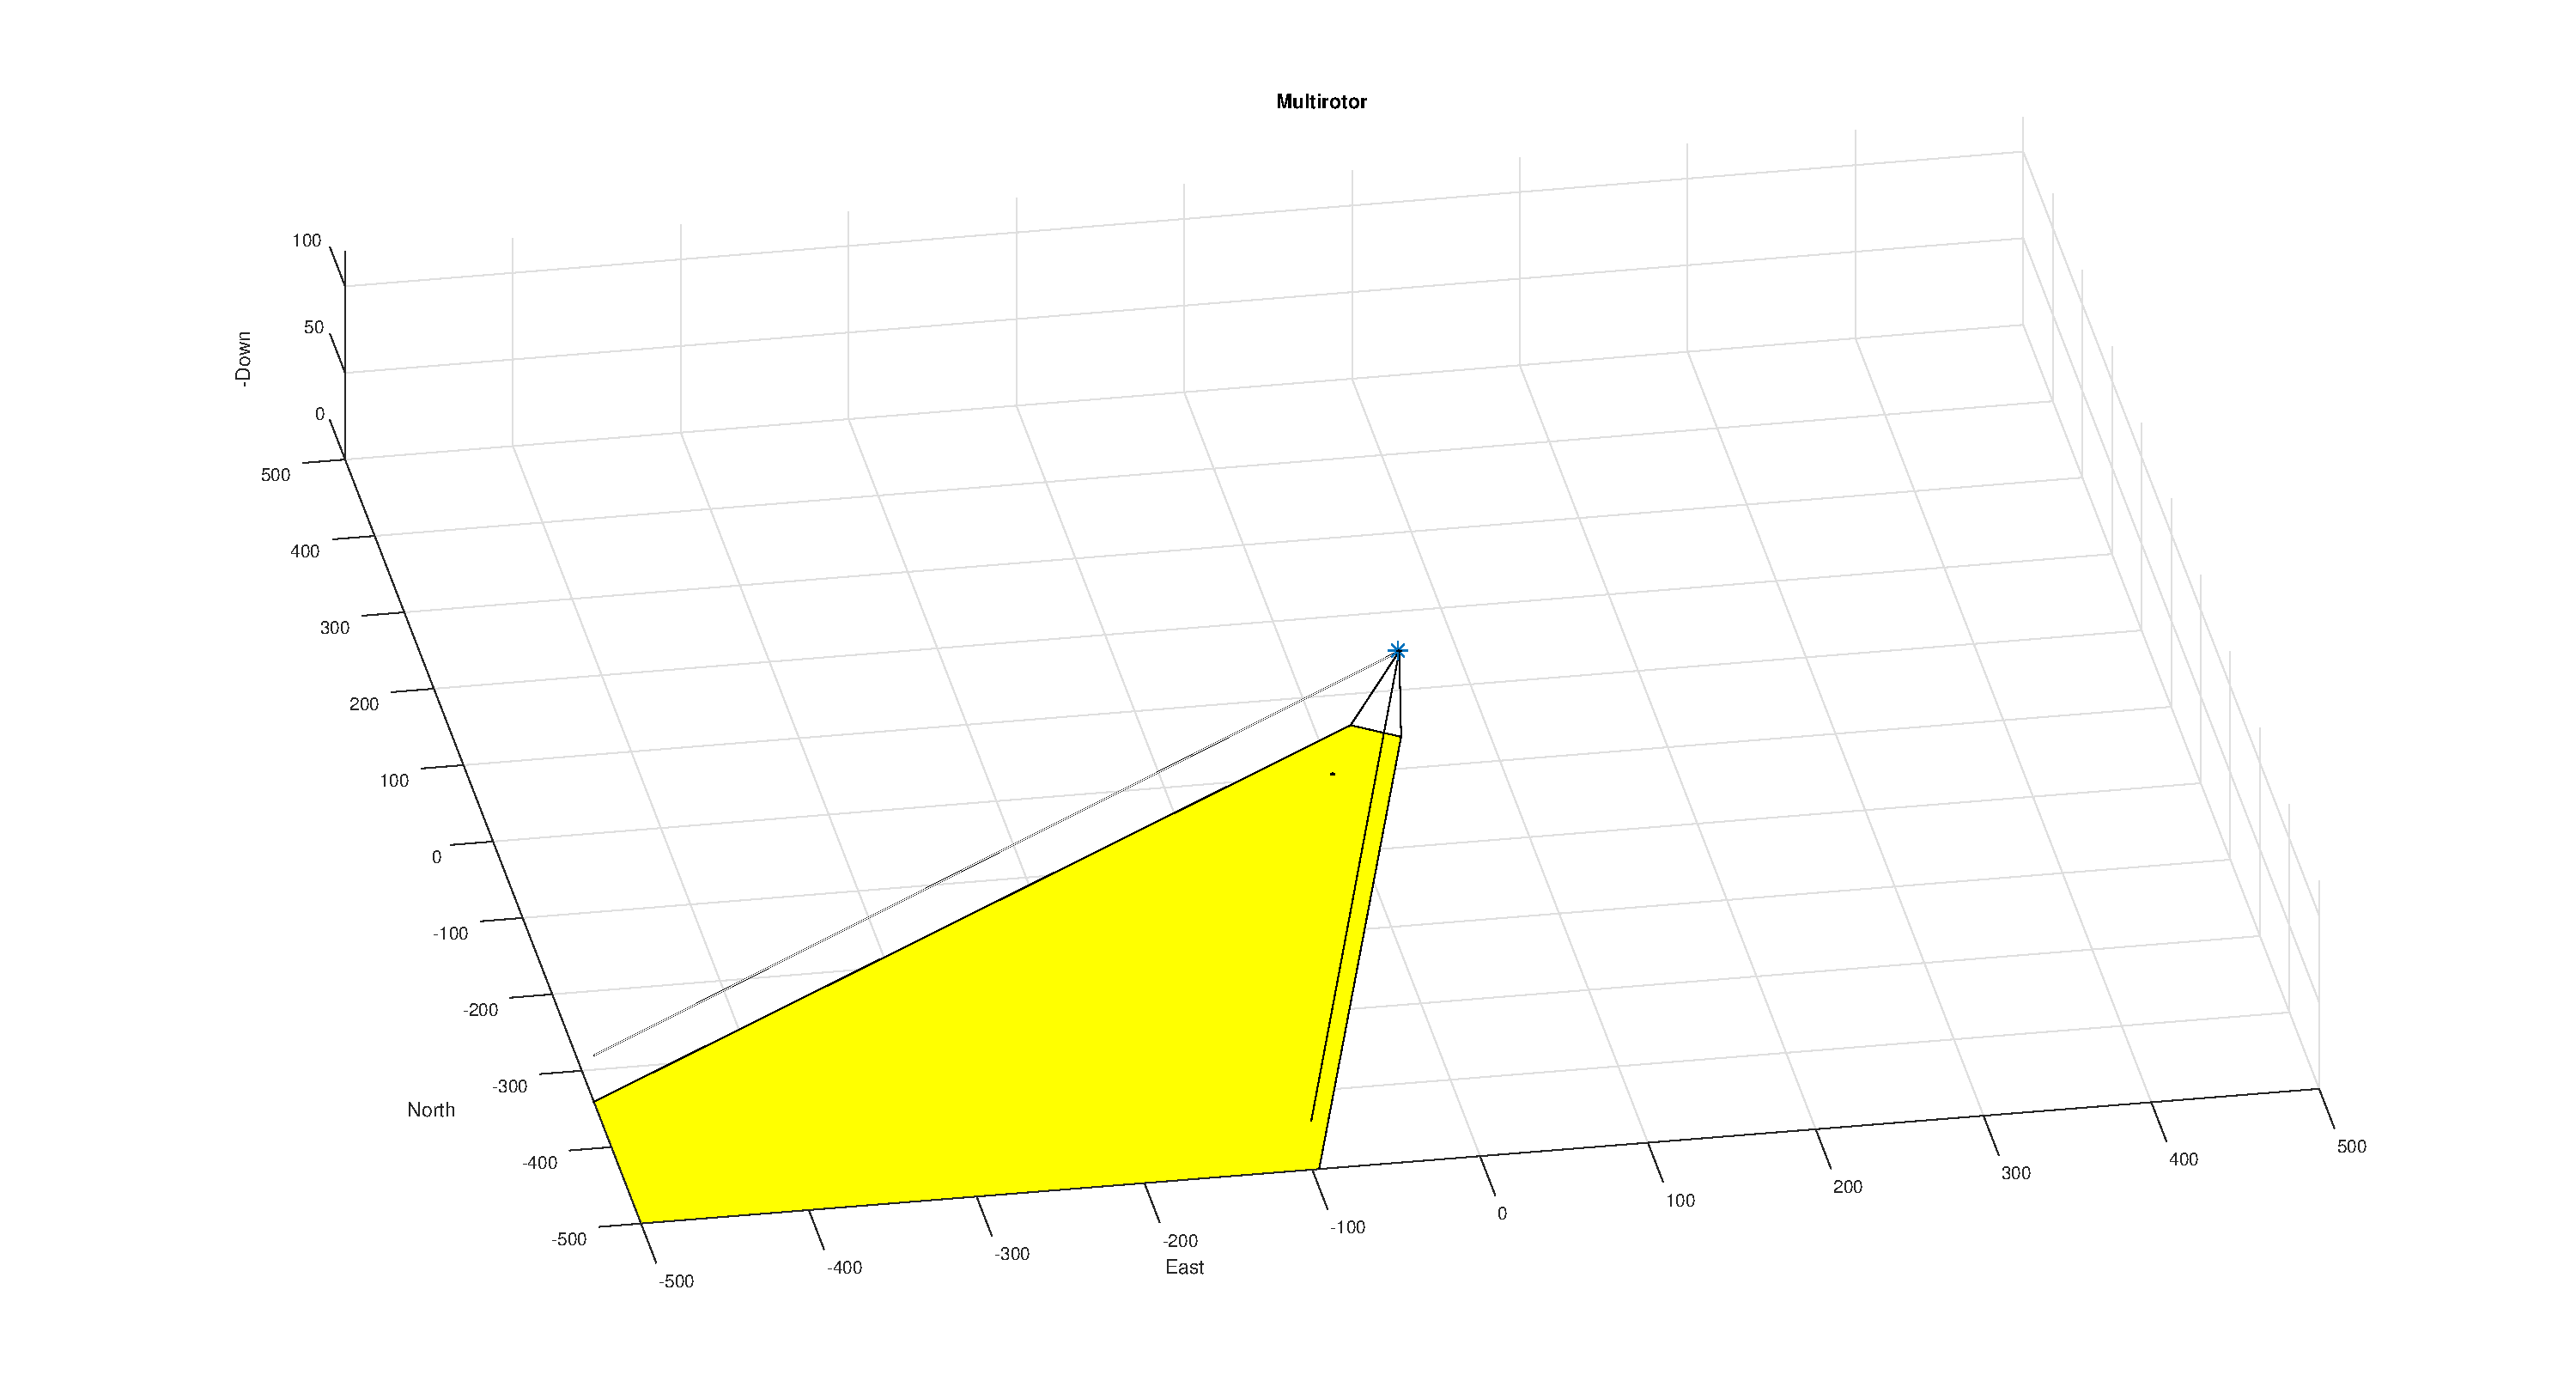
\includegraphics[height=4.5cm]{images/chapter2/uav_adaptive_60s}
		\caption{Multirotor at $t=60s$}
	\end{subfigure}%
	\begin{subfigure}{0.5\textwidth}
		\centering
		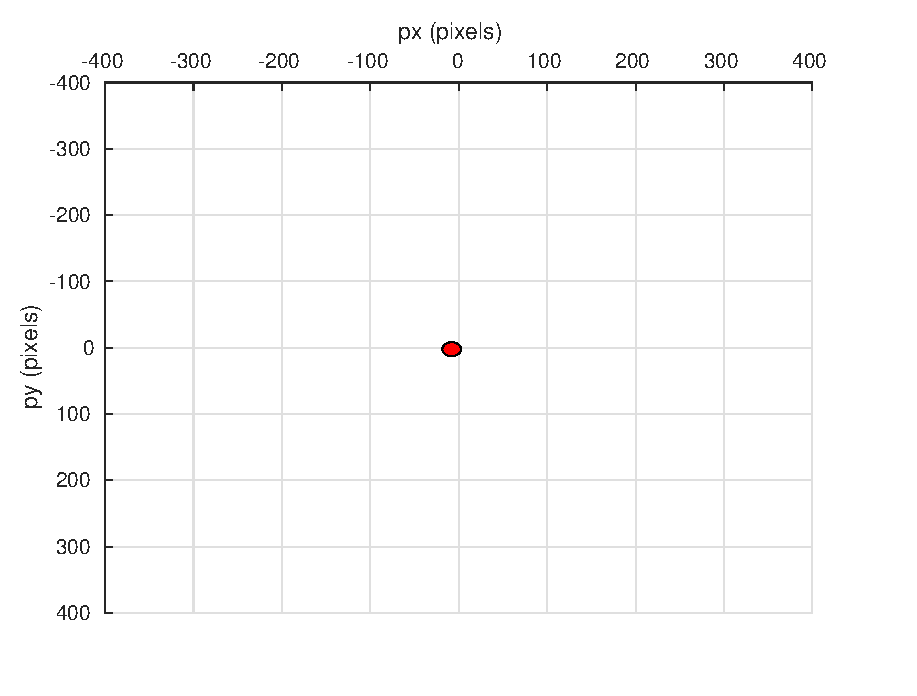
\includegraphics[height=4.5cm]{images/chapter2/camera_adaptive_60s}
		\caption{Camera view at $t=60s$}
	\end{subfigure}	
	\begin{subfigure}{0.5\textwidth}
		\centering
		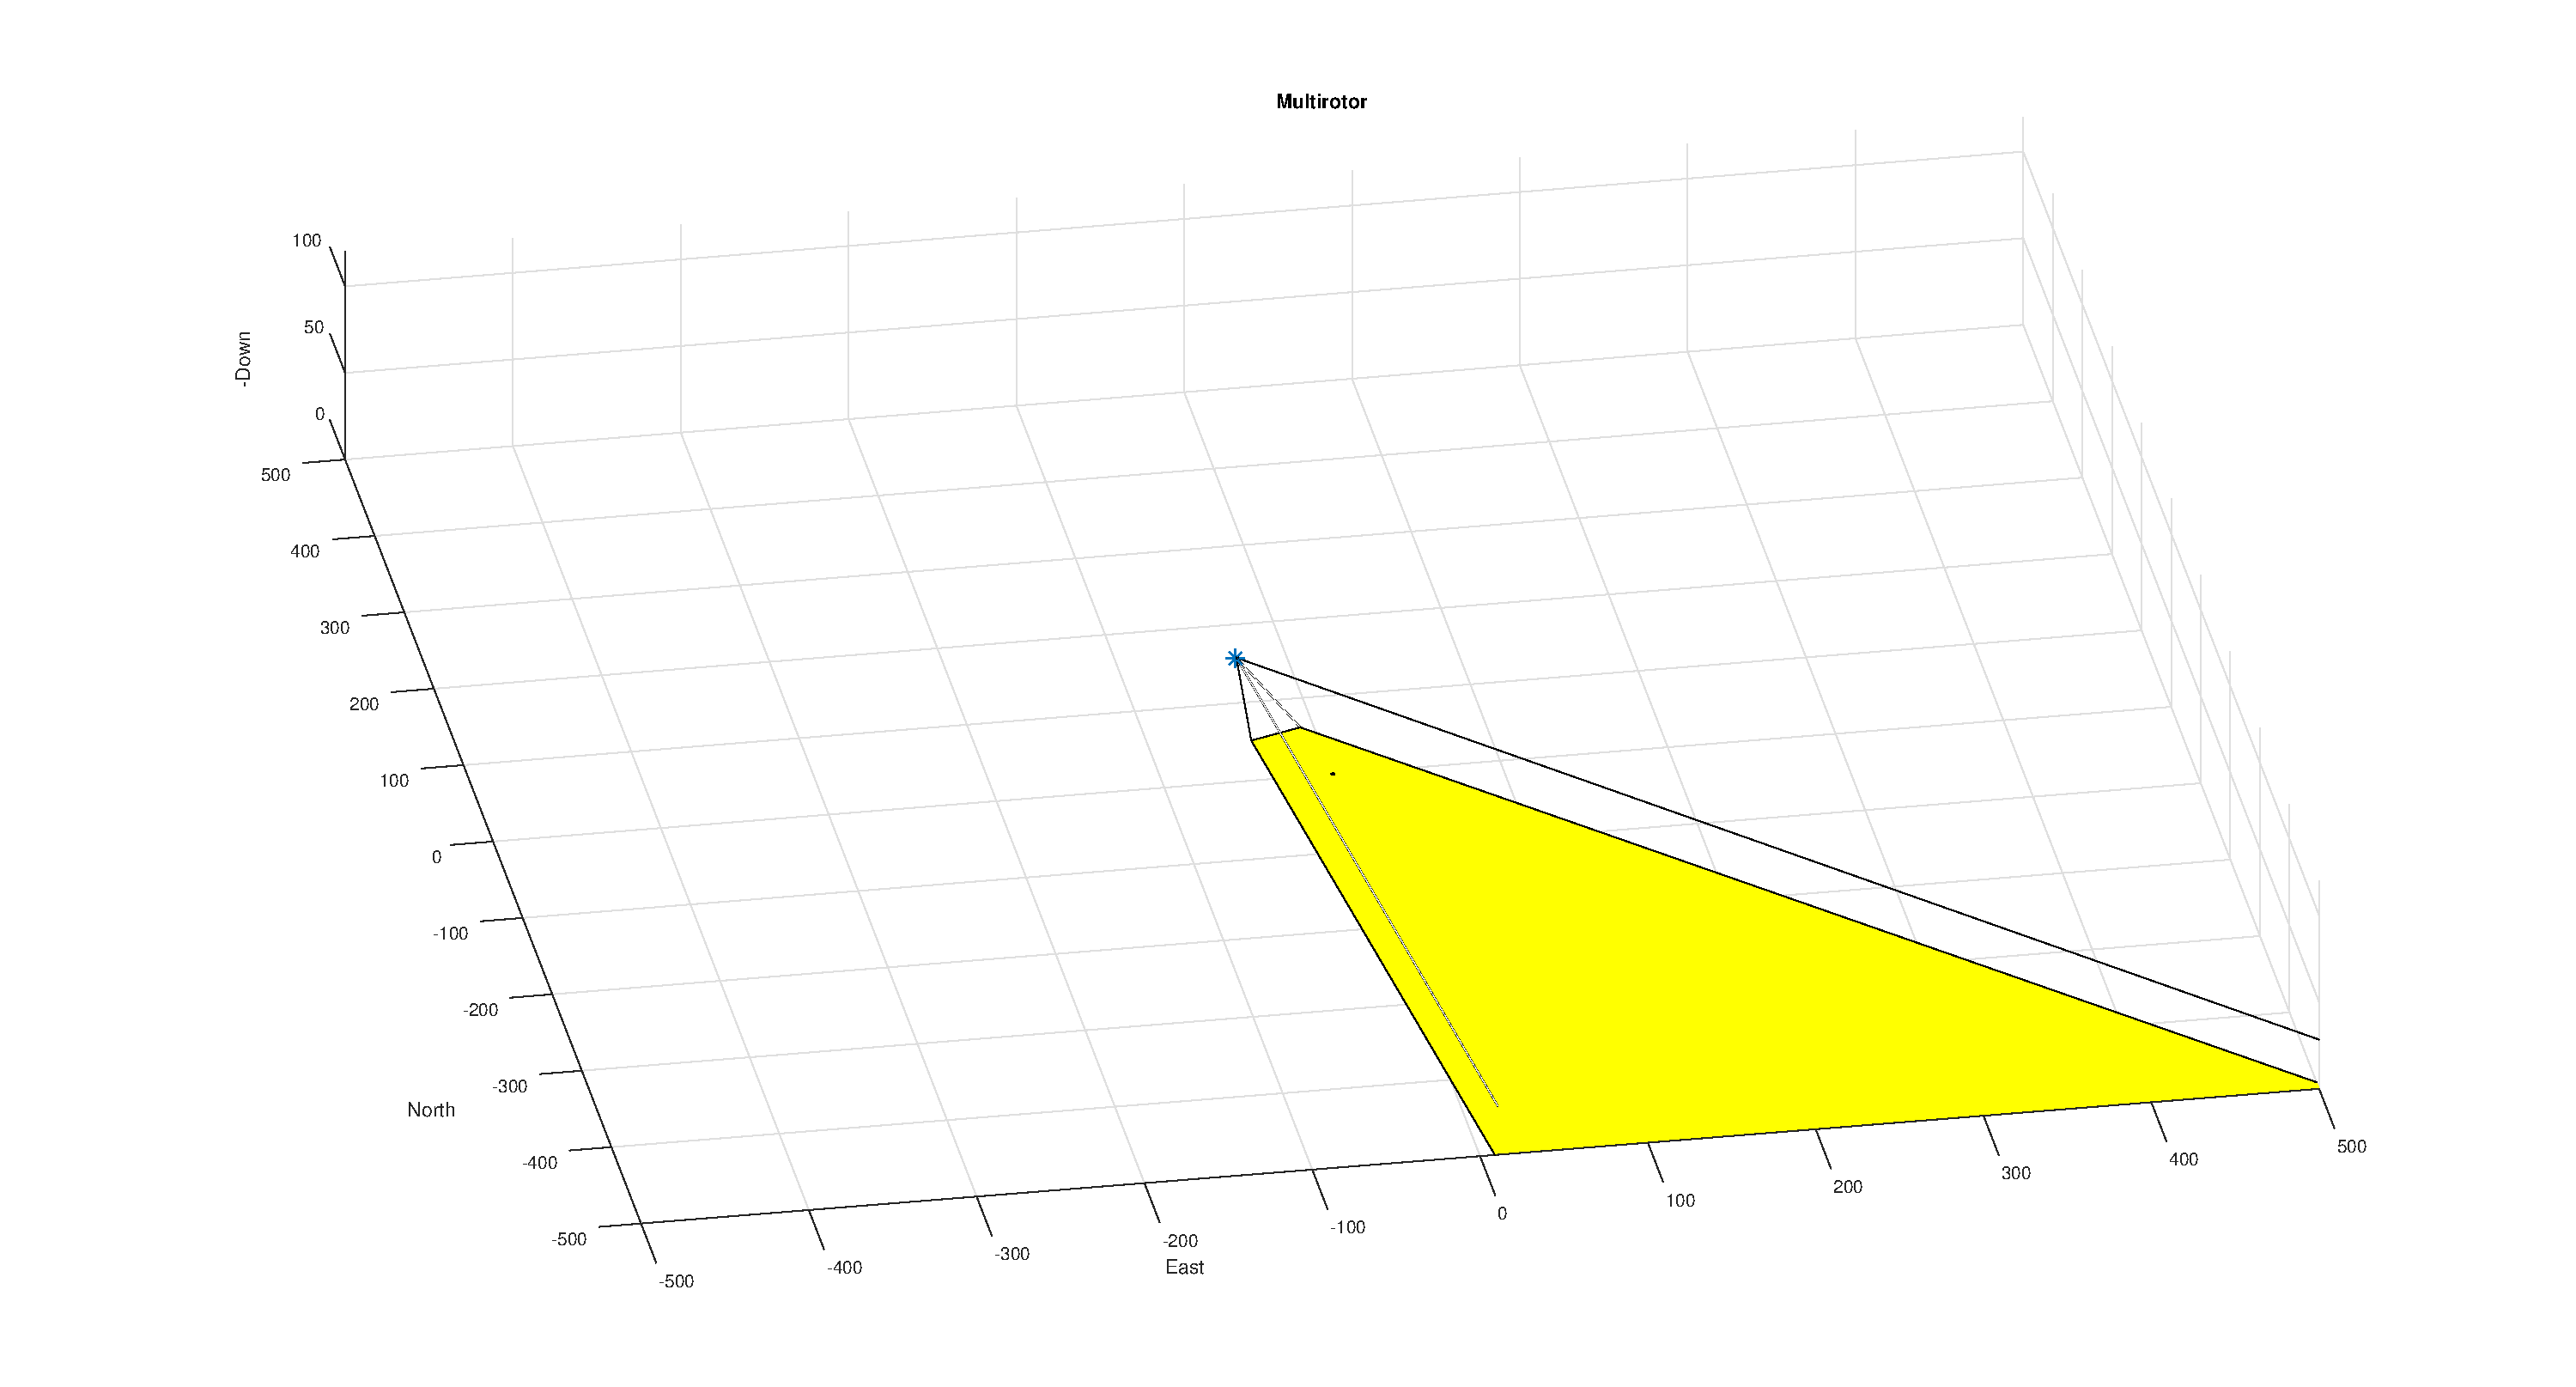
\includegraphics[height=4.5cm]{images/chapter2/uav_adaptive_120s}
		\caption{Multirotor at $t=120s$}
	\end{subfigure}%
	\begin{subfigure}{0.5\textwidth}
		\centering
		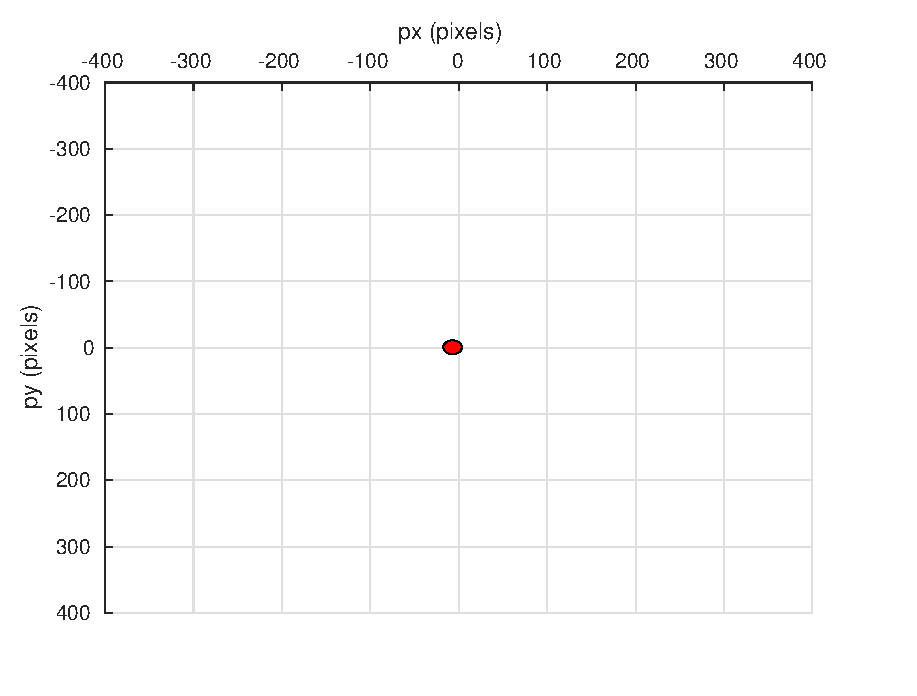
\includegraphics[height=4.5cm]{images/chapter2/camera_adaptive_120s}
		\caption{Camera view at $t=120s$}
	\end{subfigure}
	\begin{subfigure}{0.5\textwidth}
		\centering
		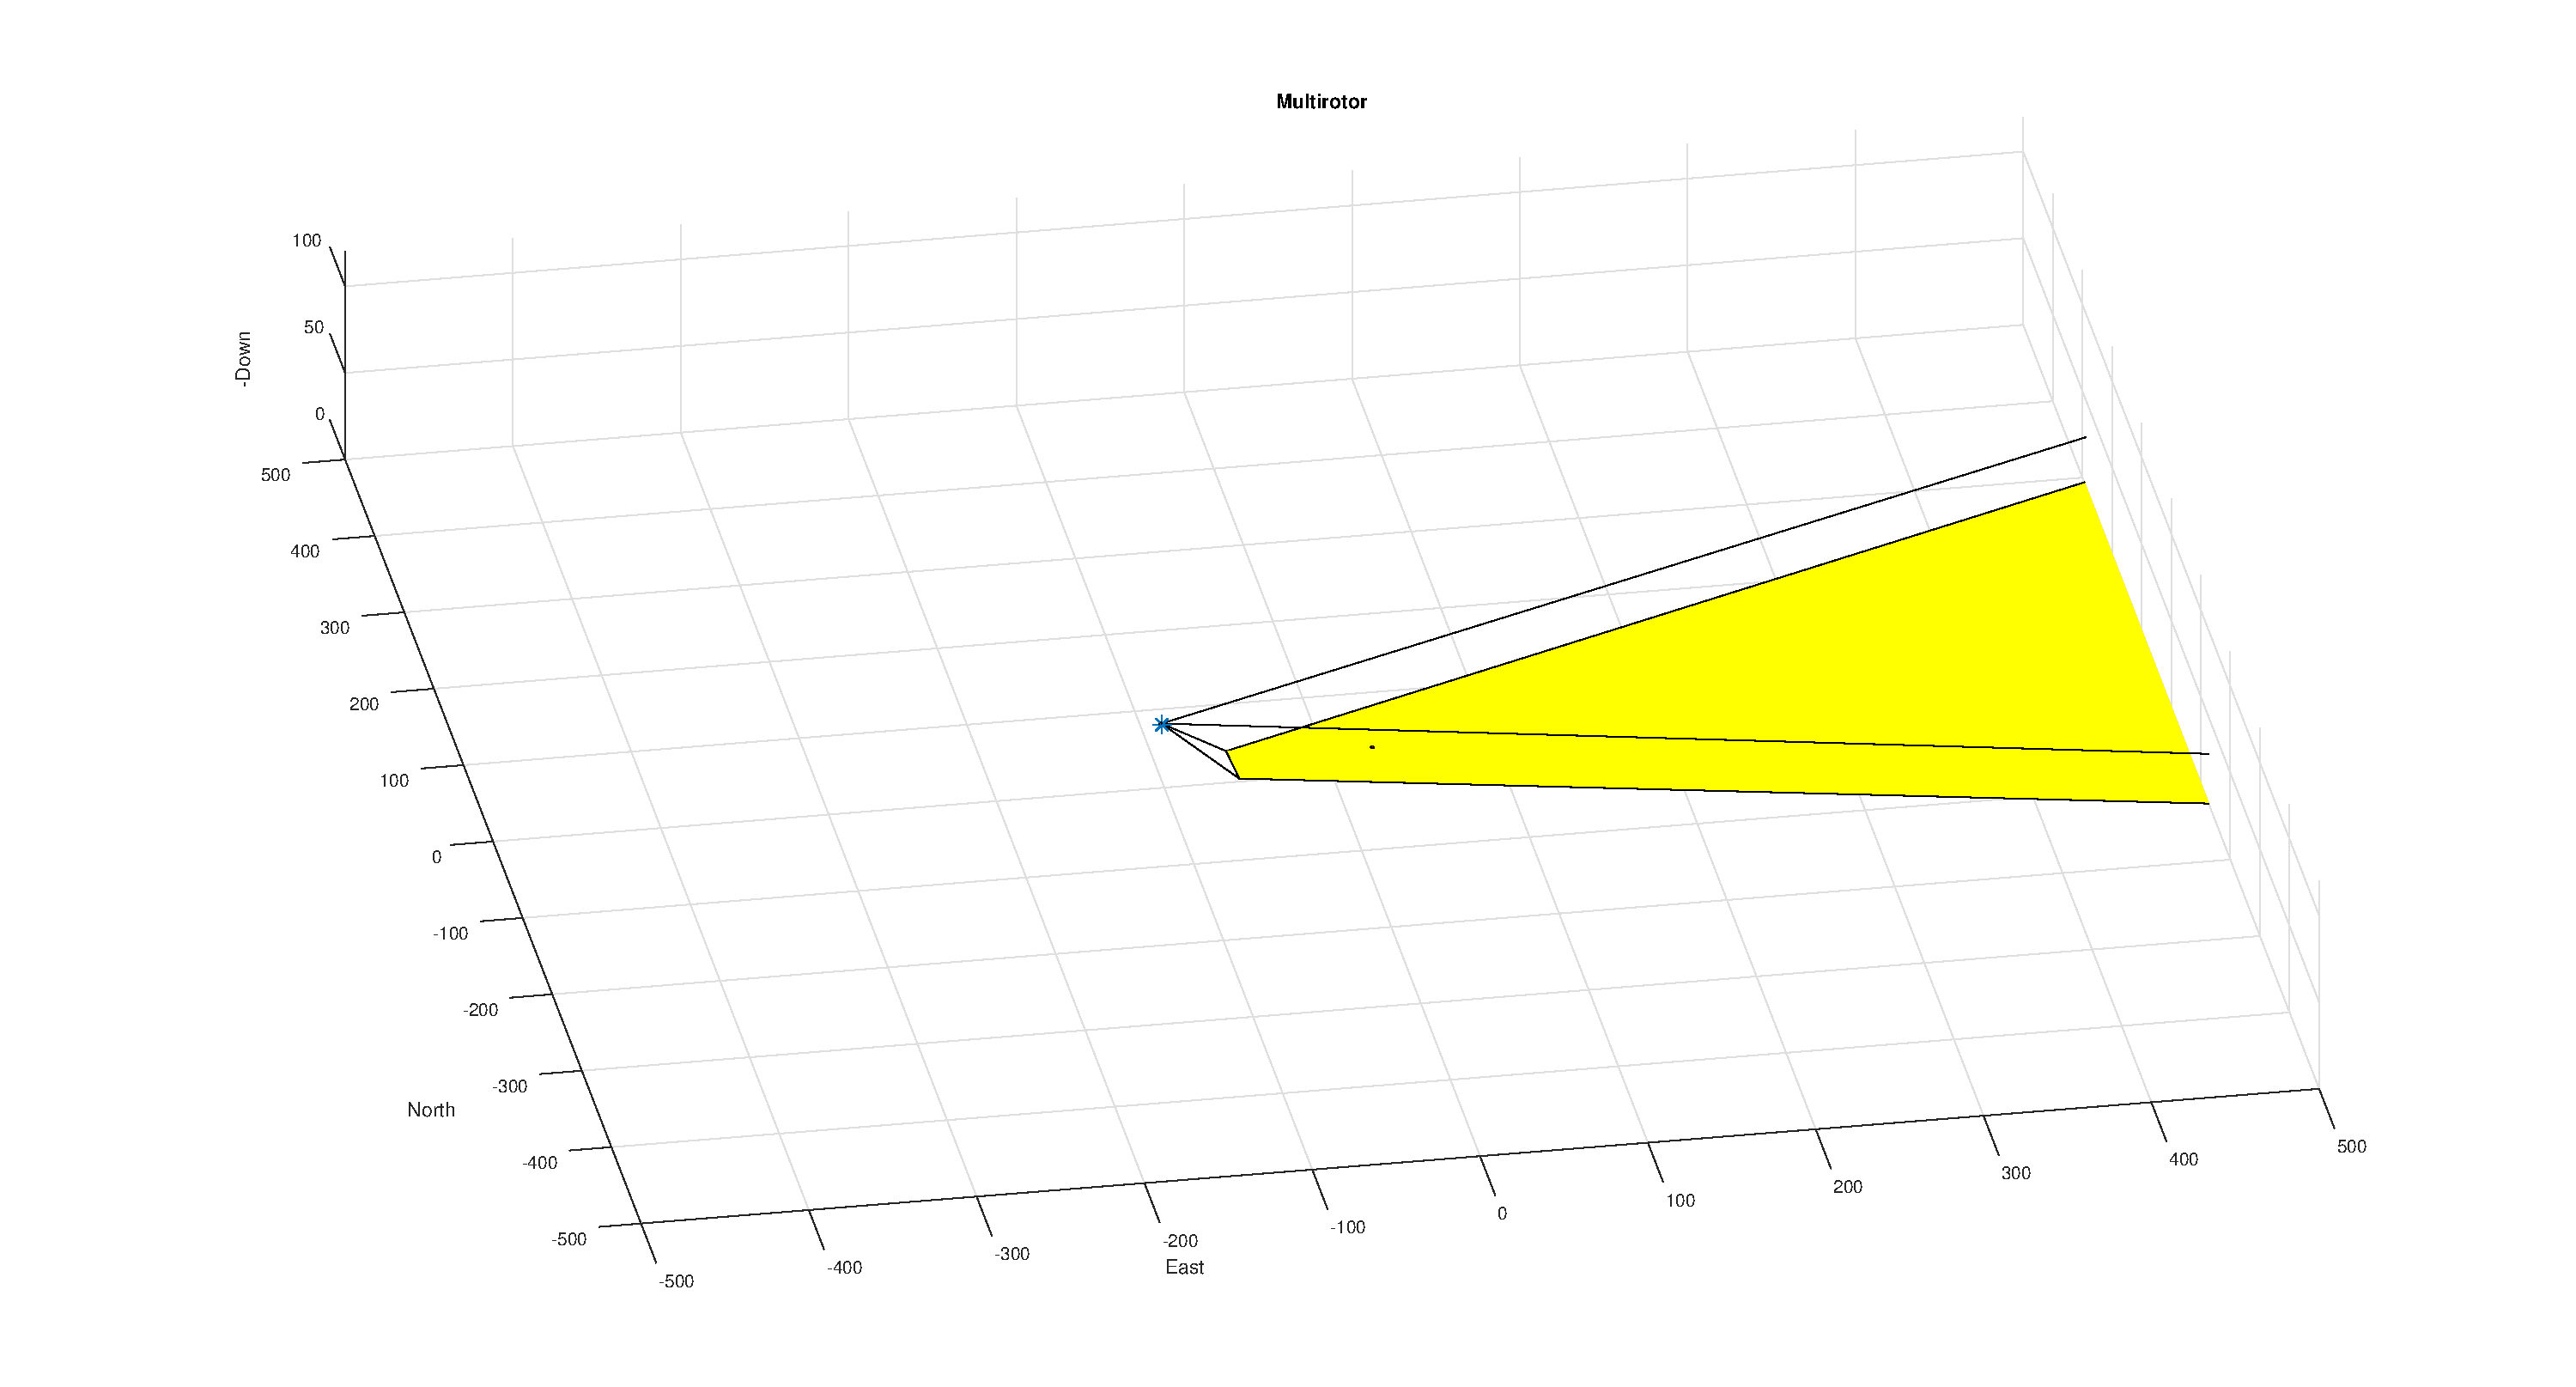
\includegraphics[height=4.5cm]{images/chapter2/uav_adaptive_180s}
		\caption{Multirotor at $t=180s$}
	\end{subfigure}%
	\begin{subfigure}{0.5\textwidth}
		\centering
		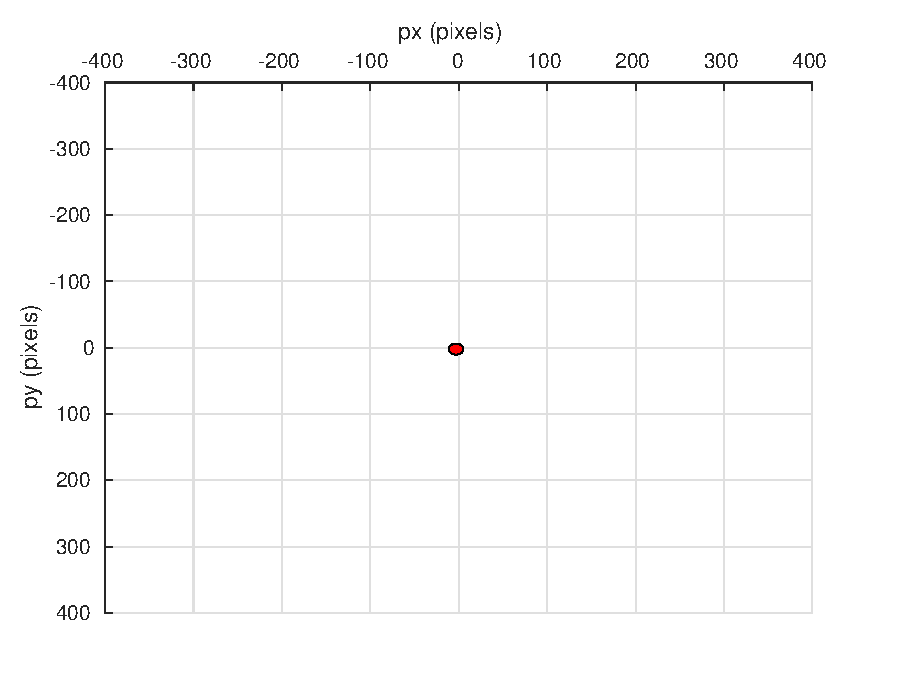
\includegraphics[height=4.5cm]{images/chapter2/camera_adaptive_180s}
		\caption{Camera view at $t=180s$}
	\end{subfigure}					
	\caption{Multirotor simulation with camera view. The gimbal pointing objective is well achieved.}
	\label{uav_adaptive}
\end{figure*}

\begin{figure*}[htbp]
	\centering
	\begin{subfigure}{0.5\textwidth}
		\centering
		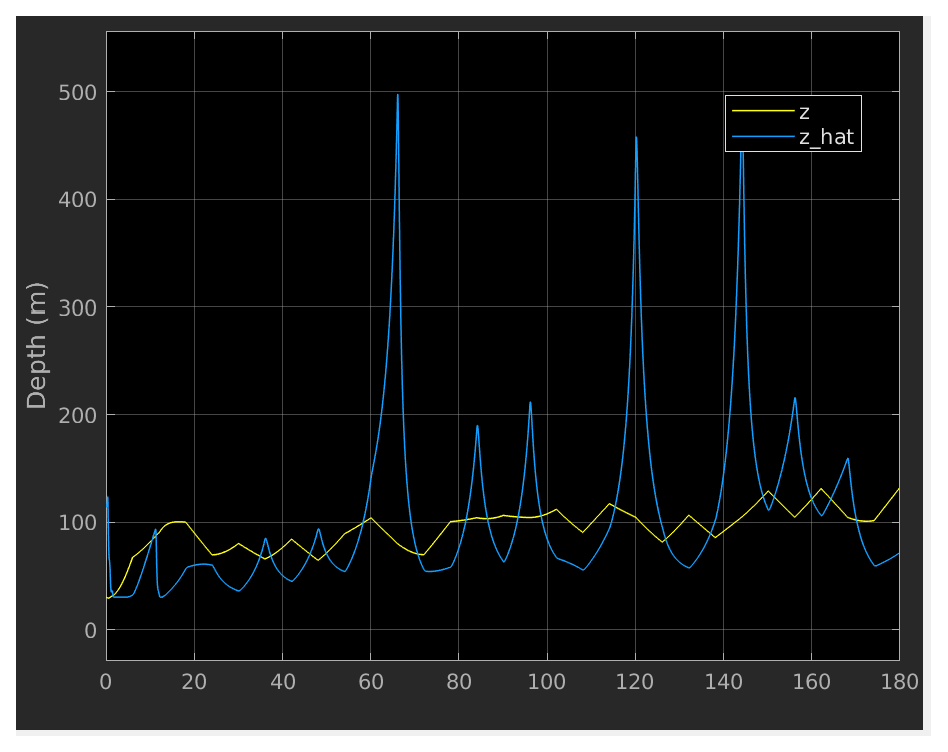
\includegraphics[width=0.9\linewidth]{images/chapter2/uav_z}
		\caption{Depth $z$ and its estimate $\hat{z}$. Uncertain parameter converging to true value is not guaranteed.}
	\end{subfigure}%
	\begin{subfigure}{0.5\textwidth}
		\centering
		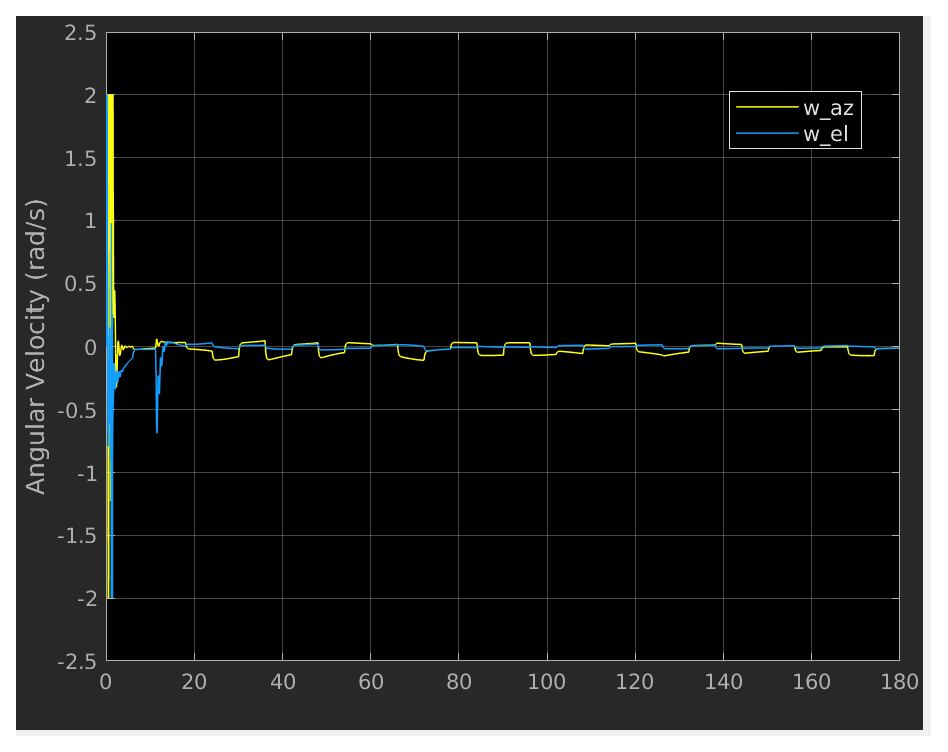
\includegraphics[width=0.9\linewidth]{images/chapter2/uav_gimbal_command}
		\caption{Angular velocity gimbal azimuth and elevation commands}
	\end{subfigure}
	\begin{subfigure}{0.5\textwidth}
		\centering
		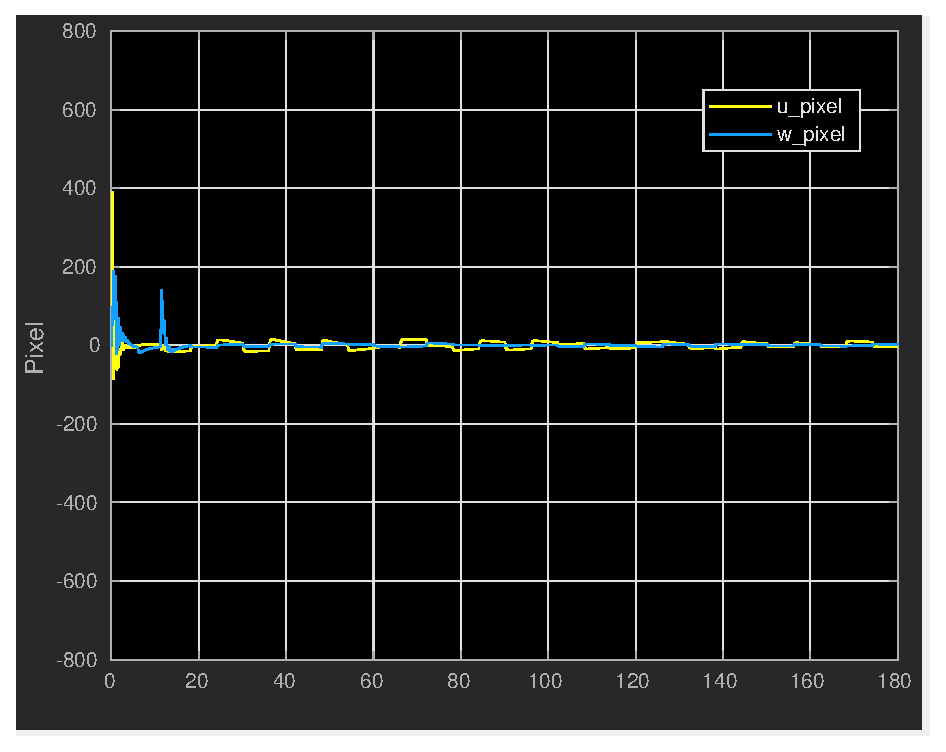
\includegraphics[width=\linewidth]{images/chapter2/uav_pixel}
		\caption{Pixel value $u$ and $w$. They are maintained around the center of the image.}
	\end{subfigure}	
	\caption{Uncertain parameter estimation, gimbal angular velocity commands from the controller, and where target lies in the image.}
	\label{uav_adaptive_additional}
\end{figure*}

\subsection{Hardware}
The adaptive depth gimbal controller is tested on the custom pan-tilt gimbal shown in Figure \ref{gimbal}. The gimbal consists of a uEye UI-3250-LE-C-HQ camera, BaseCam SimpleBGC 32-bit gimbal controller, CUI AMT203 ABS SPI encoder, Quanum 4008 precision brushless gimbal motor, and 3D printed housing (See Figure \ref{gimbal_parts}). The system block diagram can be found in Figure \ref{gimbal_blockdiagram}. The Arduino acts as a communication bridge by receiving the current azimuth and elevation angle from the encoder and passes them to the onboard computer. Also, it passes the angular velocity commands from the onboard computer to the gimbal controller. A tracking algorithm running on the onboard computer receives an image from the camera and outputs the pixel location of the target. The onboard computer also runs the controller that computes the gimbal angular velocity and passes it to the Arduino.
\begin{figure}[htbp]
	\centering
	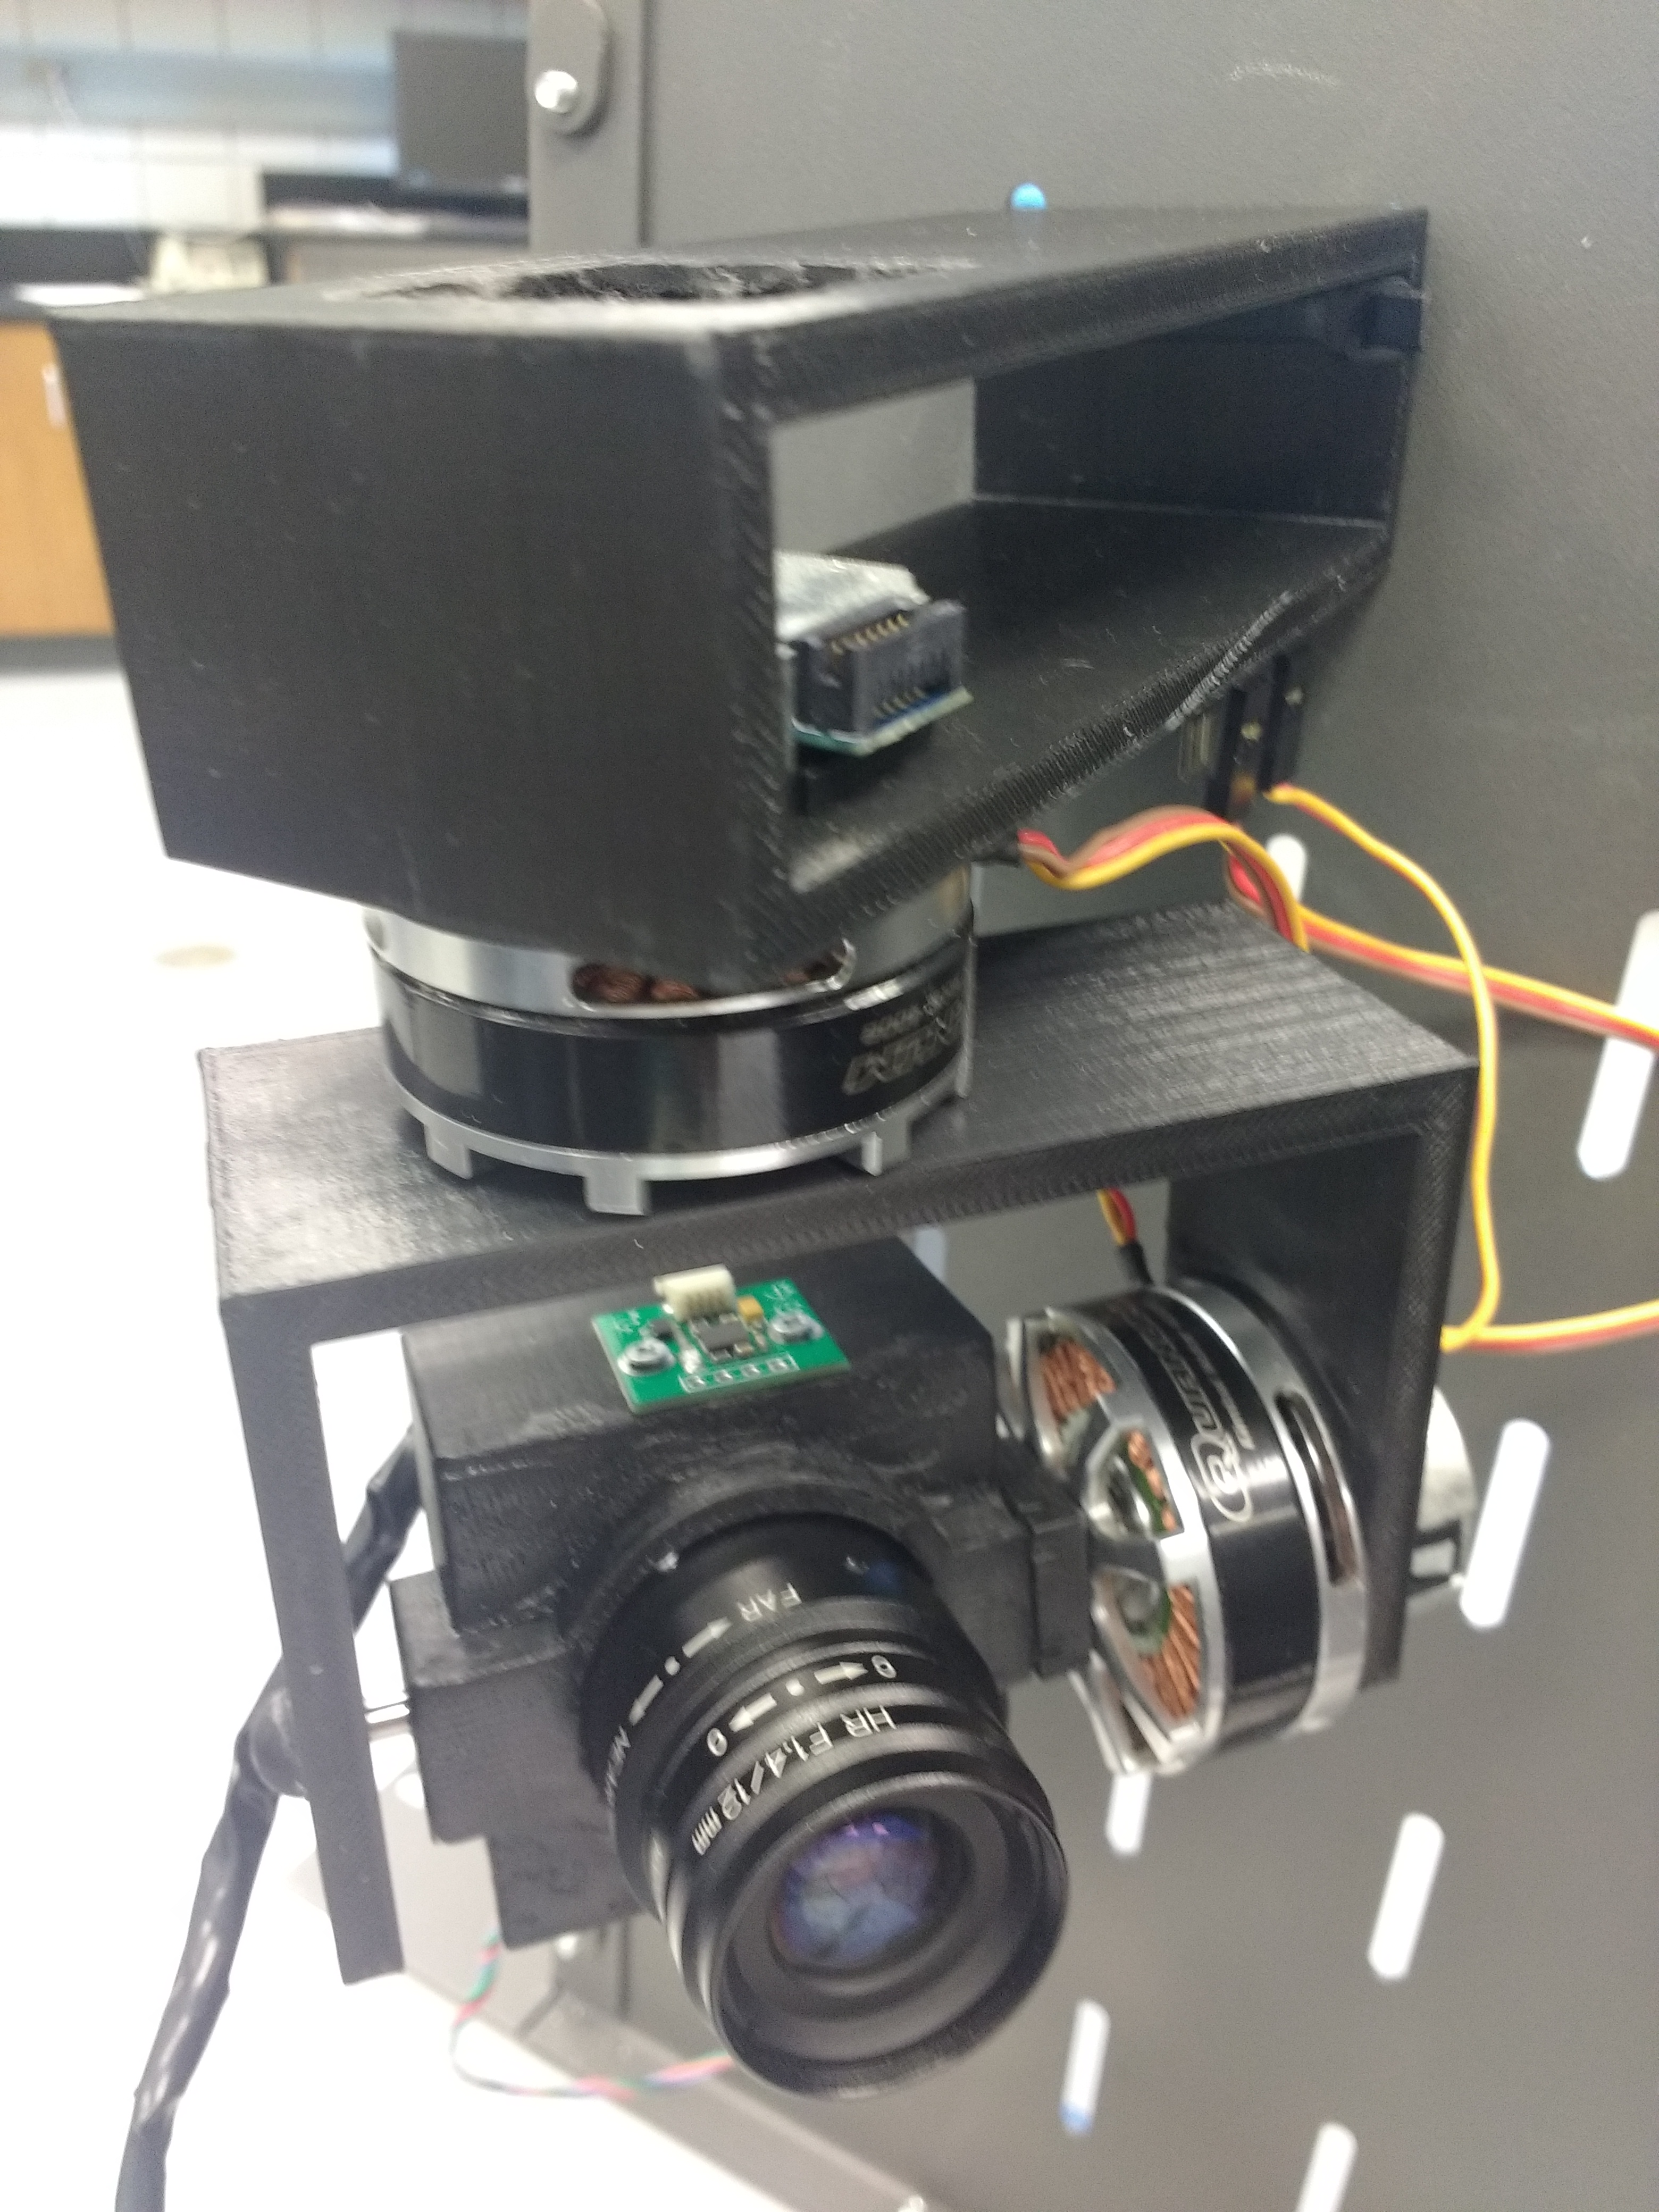
\includegraphics[height = 3in]{images/chapter2/gimbal.jpg}
	\caption{A custom pan-tilt camera gimbal}
	\label{gimbal}
\end{figure}
\begin{figure}[htbp]
	\centering
	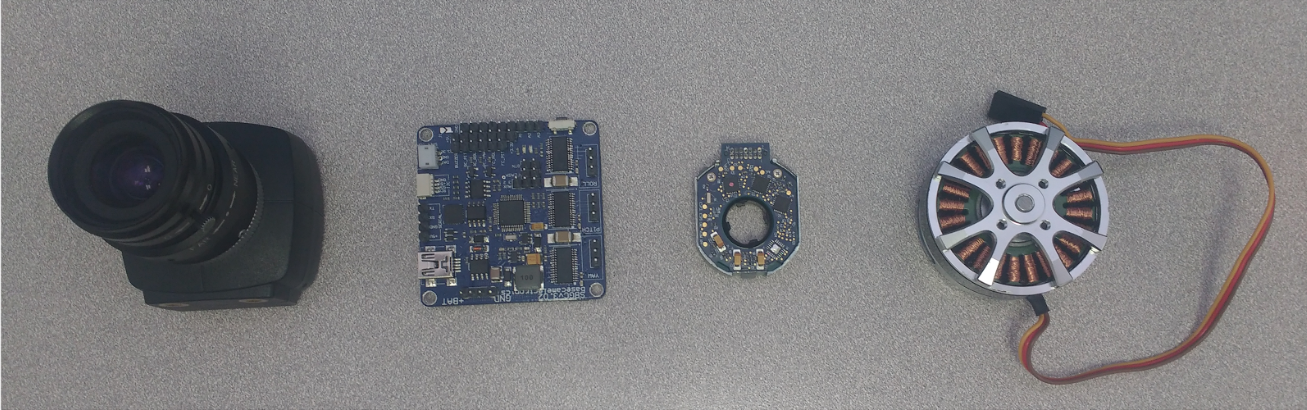
\includegraphics[width=0.8\linewidth]{images/chapter2/gimbal_parts.png}
	\caption{A custom pan-tilt camera gimbal}
	\label{gimbal_parts}
\end{figure}
\begin{figure}[htbp]
	\centering
	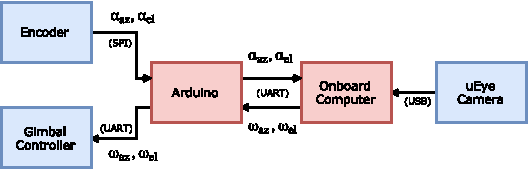
\includegraphics[width=0.8\linewidth]{images/chapter2/gimbal_system_blockdiagram}
	\caption{Custom gimbal block diagram}
	\label{gimbal_blockdiagram}
\end{figure}
A series of snapshots that shows the gimbal pointing result with the custom hardware and the adaptive depth gimbal controller are shown in Figure \ref{gimbal_hardware_result}. Also, a video showing the same result can be seen at \href{https://www.youtube.com/watch?v=VMfvQkhD9-o}{https://www.youtube.com/watch?v=VMfvQkhD9-o}. In this particular result, the camera is static which means that $v_{C}$ is set to zero.
\begin{figure*}[htbp]
	\centering
	\begin{subfigure}{0.5\textwidth}
		\centering
		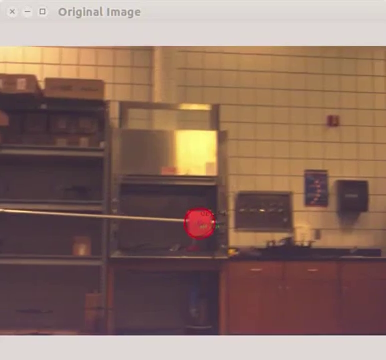
\includegraphics[height=6.5cm]{images/chapter2/gimbal_hardware_1.png}
		\caption{At $t=0s$}
	\end{subfigure}%
	\begin{subfigure}{0.5\textwidth}
		\centering
		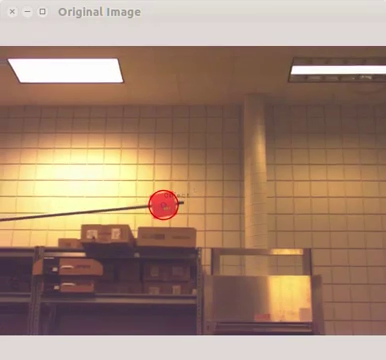
\includegraphics[height=6.5cm]{images/chapter2/gimbal_hardware_2.png}
		\caption{At $t=10s$}
	\end{subfigure}
	\begin{subfigure}{0.5\textwidth}
		\centering
		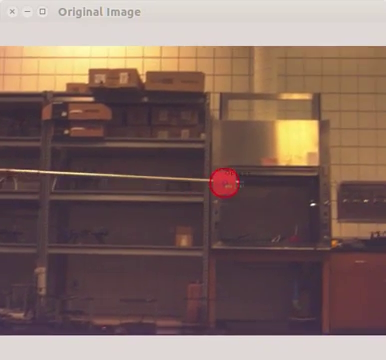
\includegraphics[height=6.5cm]{images/chapter2/gimbal_hardware_3.png}
		\caption{At $t=20s$}
	\end{subfigure}%
	\begin{subfigure}{0.5\textwidth}
		\centering
		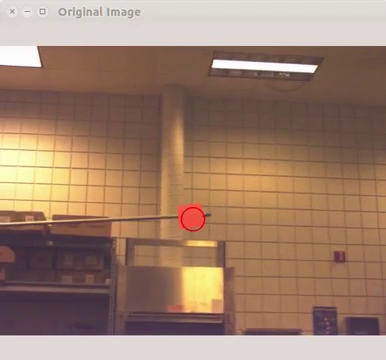
\includegraphics[height=6.5cm]{images/chapter2/gimbal_hardware_4.png}
		\caption{At $t=30s$}
	\end{subfigure}	
	\begin{subfigure}{0.5\textwidth}
		\centering
		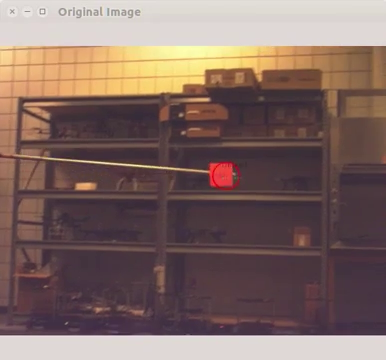
\includegraphics[height=6.5cm]{images/chapter2/gimbal_hardware_5.png}
		\caption{At $t=40s$}
	\end{subfigure}%
	\begin{subfigure}{0.5\textwidth}
		\centering
		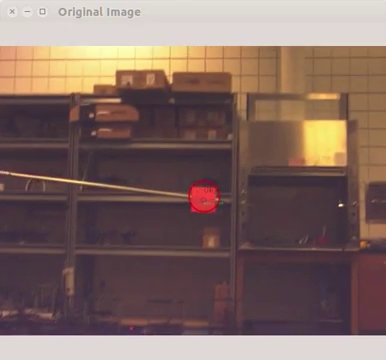
\includegraphics[height=6.5cm]{images/chapter2/gimbal_hardware_6.png}
		\caption{At $t=50s$}
	\end{subfigure}	
	\caption{Adaptive depth gimbal control result on the custom-built hardware.}
	\label{gimbal_hardware_result}
\end{figure*}

\section{Conclusion}
There are a few controller options to keep a target in the camera field of view using a gimbal. Depending on whether the camera is moving or stationary, either angle commanding gimbal control (ACGC) or angular velocity commanding gimbal control (AVCGC) can be used. The advantage of the ACGC is that it is easy to implement and that it does not require the depth information. The AVCGC is expected to perform better than ACGC for a moving camera since the AVCGC take the moving platform into account. However, the AVCGC requires knowledge of the depth $z$. When there is no way to reliably measure or estimate the depth $z$, the adaptive depth gimbal control (ADGC) can be used. A summary is shown in Table \ref{gimbal_summary}.
\begin{table}[htbp]
	\begin{tabular}{ |c|c|c| } 
		\hline
		ACGC & AVCGC & ADGC \\
		\hline
		Easy to implement & Designed for moving camera & Designed for moving camera \\ 
		Designed for static camera & Requires the knowledge of the depth $z$ & Works without knowing $z$ \\  
		\hline
	\end{tabular}
	\caption{Summary of gimbal control schemes}
	\label{gimbal_summary}
\end{table}
\chapter{Autonomous Target Following System}
\label{chapter3}
This chapter presents a vision-based target tracking and following system using a monocular camera on an Unmanned Aerial System (UAS). The Recursive-RANSAC (R-RANSAC) tracker tracks multiple moving objects in the camera field of view and the proposed controller is capable of following a particular target selected by a user while keeping the target in the center of the image. The main contribution of this work is that multiple objects can be tracked without imposing restrictions such as color, shape, etc. Also, the hardware test shows that the system is able to follow a target autonomously in a real-world outdoor environment.

\section{System Overview}
\begin{figure}[htbp]
	\centering
	\framebox{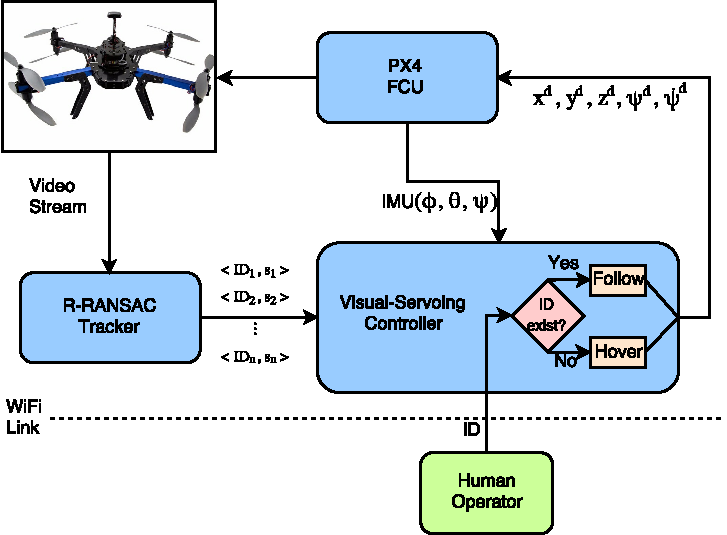
\includegraphics[width=0.6\textwidth]{images/chapter3/system_diagram.pdf}}
	\caption[Autonomous target following system architecture.]{Autonomous target following system architecture. The R-RANSAC tracker produces a set of target ID numbers and corresponding pixel locations. The visual-servoing controller outputs the desired position, heading, and yaw rate based on the pixel location of the requested target.}
	\label{system}
\end{figure}
The R-RANSAC tracker and the visual-servoing controller are major subsystems as shown in Figure \ref{system} and they communicate using the Robot Operating System (ROS) framework. The Pixhawk flight controller is used with the PX4 firmware for the autopilot. The R-RANSAC tracker is responsible for tracking moving objects in the image sequence and outputs a vector of normalized image coordinates with unique ID assigned to each track. Let the normalized pixel coordinates be defined as 
\begin{equation}
s = [\epsilon_x, \epsilon_y],
\end{equation} where $\epsilon_x$, $\epsilon_y$ are normalized pixel coordinates. Combined with IDs, a vector of track information is defined as 
\begin{equation}
T = [<ID_1, s_1>, <ID_2, s_2>, \dots, <ID_n, s_n>].
\end{equation}
The human operator assigns which target the UAV is to follow by sending a target ID number using the ground station. The controller checks to see if the target with the same ID given by the human operator exists among tracks. If the target exists, the controller keeps the target in the center of the image by commanding yaw rate and forward, backward motion of the UAV. Otherwise, the controller holds the UAV's current position until it receives another target ID existing among tracks. 

\section{Recursive-RANSAC Tracker}
This section describes the visual detection and tracking framework. The objective of the visual tracker is to reliably track all targets in the field of view such that the ground operator can select a desired ID number for visual servoing. All elements of target tracking are required to be autonomous, without a priori knowledge of the number of targets in the field of view. A key requirement is track continuity (persistent track ID numbers) in order for the system to achieve good following performance. An ID-loss event requires the ground operator to select the new target ID when the track is re-initialized which leads to undesirable flight behavior. No detection aids such as color segmentation or truth data are available to the controller, meaning that target detection and state estimation must be robust in standard flight environments.
\begin{figure}[htbp]
	\centering
	\framebox{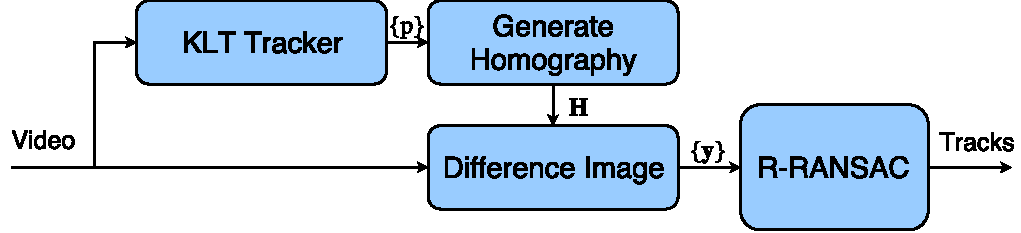
\includegraphics[width=0.8\textwidth]{images/chapter3/tracker_diagram.pdf}}
	\caption[The detection framework used to generate measurements used by R-RANSAC.]{The detection framework used to generate measurements used by R-RANSAC. The KLT tracker creates point correspondences between frames which are used to calculate a homography. The difference image detects motion in the frame and creates position measurements of potential targets.}
	\label{visual_tracking}
\end{figure}

Difference imaging reveals motion in the field of view by warping the previous image into the current image and comparing the two frames. This approach was used because it tends to be more robust in the presence of noisy homography transforms and image imperfections experienced by rolling shutter cameras in the presence of vibration. Our flight demonstration used entry-level hardware such as a webcam without gimbal stabalization.

This form of motion detection requires knowledge of the homography as seen in Figure \ref{visual_tracking}. The KLT algorithm is used to create point correspondences across the image and the homography is generated from these points using a RANSAC method.

R-RANSAC is an MTT algorithm that generates many hypothesis trajectories based upon an assumed dynamic model of the targets and the set of recent measurements. By elevating models that surpass a threshold of inlier measurements, the algorithm is capable of tracking many targets with missed detections in clutter \cite{Niedfeldt2014}.

For each new set of measurements, those that are inliers to existing models are used to perform a Kalman update using a probabalistic data association (PDA) filter. For each measurement that is an outlier to all existing models, a new model is generated by sampling trajectories based on the recent history of measurements. The trajectory hypothesis with the most inliers is selected as a new model and the inlier measurements are used to estimate the target state estiamate and error covariance for the current timestep. Additional operations perform model merging and pruning in order to eliminate unlikely models.

By using the difference image measurements and R-RANSAC, track ID numbers are produced for targets in the field of view and can be used for visual servoing operations.

\section{UAV Control}
The visual tracking system in the previous section provides the control algorithm with a vector of normalized image coordinates for every track in the camera field of view. The control algorithm activates follow mode when there exists a target with the ID that a human operator has assigned for following. When the given ID is not found in the vector that the tracker provides, the control algorithm commands the UAV to hold its position until another target ID that exists among the tracks is assigned to follow. In this section, the control algorithm is described in more detail.

\subsection{Coordinate Frame Convention}
Before giving a detailed explanation of the control algorithm, it is worth clarifying our assumptions and the coordinate frames used. 

First, an East-North-Up (ENU) coordinate frame is used as opposed to the common North-East-Down (NED) coordinates for UAV in order to match the frame convention used in the \texttt{mavros} package in ROS \cite{mavros}. Let $\mathcal{F}^i$ be the inertial frame, which in this case coincides with the ENU frame, and let $\mathcal{F}^v$ be the vehicle frame that is translated to the UAV center of mass, with the same orientation as $\mathcal{F}^i$. Vehicle-1 frame, $\mathcal{F}^{v1}$ indicates the frame that is only rotated about the $z$-axis of $\mathcal{F}^{v}$ by $\psi$, the heading angle of the multirotor. The rotation matrix from $\mathcal{F}^v$ to $\mathcal{F}^{v1}$ can be expressed as $R^{v1}_v$. Other involved frames are the optical, camera, and body frames expressed as $\mathcal{F}^o$, $\mathcal{F}^c$, $\mathcal{F}^b$, respectively. 

Second, a flat-earth model is used to properly scale the target position relative to the camera in $\mathcal{F}^{v1}$ and we assume that we have access to the correct altitude information. 

Third, the displacement between the center of mass of the UAV and the focal point of the camera is ignored since it is negligible compared to the distance between the camera and the target. 

Fourth, we will rely on the GPS position controller on the autopilot. The visual-servoing controller in this work computes the desired multirotor position in order to follow the target and send the position command to the autopilot. The control algorithm computes the desired multirotor velocity command in the vehicle-1 frame, but it is converted to a position command as a matter of convenience to interface with the Pixhawk autopilot.

\subsection{Forward and Heading Motion Control}
\begin{figure}[thpb]
	\centering
	\framebox{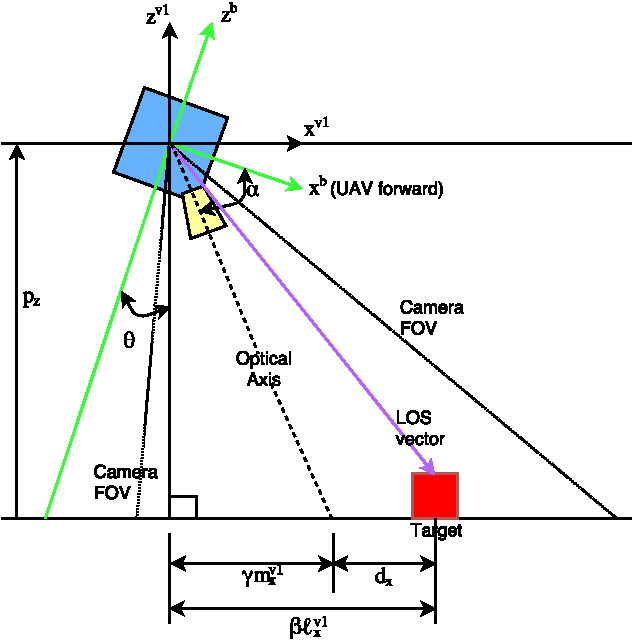
\includegraphics[width=0.5\textwidth]{images/side_view_45deg_2.pdf}}
	\caption{Side view of the multirotor.}
	\label{side_view}
\end{figure}
The first step of the motion control is to transform the line of sight (LOS) vector to the target from $\mathcal{F}^o$ to $\mathcal{F}^{v1}$ (See Figure \ref{side_view}). Let 
\begin{equation}
\mathbf{\ell}^o=[\epsilon_x^o, \epsilon_y^o, 1]^\top,
\end{equation} where $\ell^o$ is the line of sight vector in $\mathcal{F}^o$ placed at the focal length of 1. Let also the unit vector along the optical axis in $\mathcal{F}^o$ be defined as 
\begin{equation}
\mathbf{m}^o=[0, 0, 1]^\top.
\end{equation}
By applying sequential transformations to $\ell^o$ and $\mathbf{m}^o$, we get
\begin{equation}
\mathbf{\ell}^{v1}=R^{v1}_b(\phi,\theta)R^b_c(\alpha)R^c_o\ell^o=[\ell^{v1}_x, \ell^{v1}_y, \ell^{v1}_z]^\top
\end{equation}
\begin{equation}
\mathbf{m}^{v1}=R^{v1}_b(\phi,\theta)R^b_c(\alpha)R^c_o\mathbf{m}^o=[m^{v1}_x, m^{v1}_y, m^{v1}_z]^\top,
\end{equation} where $R^b_c$ is a matrix with fixed values depending on how the camera is mounted with respect to $\mathcal{F}^b$, and $R^{v1}_b$ is a matrix requiring the roll and pitch angles of the multirotor. The vector $\ell^{v1}$ is the displacement of the target relative to the multirotor and $\mathbf{m}^{v1}$ is the optical axis in $\mathcal{F}^{v1}$. The LOS vector $\ell^{v1}$ and $\mathbf{m}^{v1}$ do not have proper scalings due to the unknown depth information to the target in $\mathcal{F}^o$, but can be recovered using the altitude of the camera. Let
\begin{equation}
\beta=\frac{p_z}{\ell^{v1}_z}
\end{equation} 
\begin{equation}
\gamma=\frac{p_z}{m^{v1}_z},
\end{equation} where $p_z$ is the altitude of the multirotor. Then, the desired forward position from the current multirotor position can be computed as 
\begin{equation}
d_x=\beta\ell^{v1}_x-\gamma{m}^{v1}_x.
\end{equation}
This $d_x$ may be decomposed into east and north components as
\begin{equation}
d_n=d_x\sin(\psi)
\end{equation}
\begin{equation}
d_e=d_x\cos(\psi),
\end{equation} where $\psi$ is the heading of the multirotor. These north and east components are added to the current multirotor east and north positions, and the sum is sent to the autopilot position controller.

It is more suitable to compensate for a target moving horizontally in the image plane by adjusting the multirotor's heading than through lateral motion. Thus, a yaw rate command $\omega_z$ can be computed as 
\begin{equation}
\omega_z=\eta \ell^{v1}_y,
\end{equation} where $\eta>0$ is a control gain.

\section{Experiments and Results}
The hardware is comprised of a 3DR X8 multirotor platform, a small form factor Gigabyte BRIX GB-BXi7-4500 (no GPU), low-cost USB camera, ELP-USBFHD01M-L21 (rolling shutter), and Pixhawk with PX4 firmware. The proposed system was tested in an outdoor environment to track realistic targets (people). We demonstrate the ability to follow one of the multiple tracked objects while switching the target of interest in real-time. The tracker does not have any prior information about what tracks look like and how they might move. The hardware result shows that the R-RANSAC tracker is able to track multiple targets and to provide the controller with proper coordinates of the targets. It also shows that the controller is able to follow one of the targets while keeping it in the camera field of view.
\begin{figure}[htbp]
	\begin{subfigure}{0.48\linewidth}
		\centering
		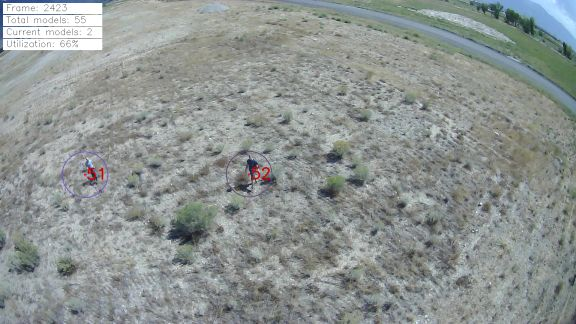
\includegraphics[width=0.95\textwidth]{images/chapter3/ID51_track_begin.png}
		\caption{Track ID 51 initiated by R-RANSAC tracker ($t=0$ s)}
		\label{camera1}
	\end{subfigure}
	\begin{subfigure}{0.48\linewidth}
		\centering
		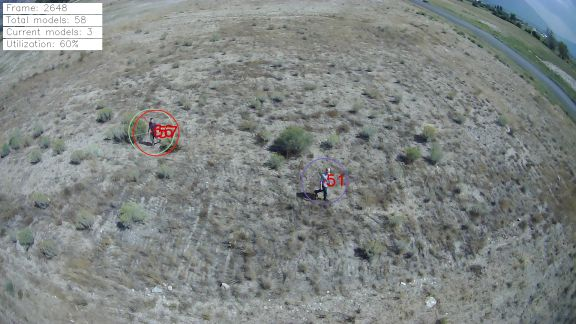
\includegraphics[width=0.95\textwidth]{images/chapter3/ID51_follow_begin.png}
		\caption{The human operator has commanded the UAV to follow track ID 51 ($t=13$ s)}
		\label{camera2}
	\end{subfigure}
	\begin{subfigure}{0.48\linewidth}
		\centering
		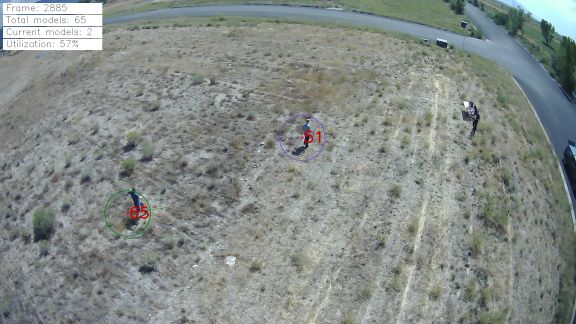
\includegraphics[width=0.95\textwidth]{images/chapter3/ID65_track_begin.png}
		\caption{Track ID 65 initiated by R-RANSAC tracker ($t=27$ s)}
		\label{camera3}
	\end{subfigure}
	\begin{subfigure}{0.48\linewidth}
		\centering
		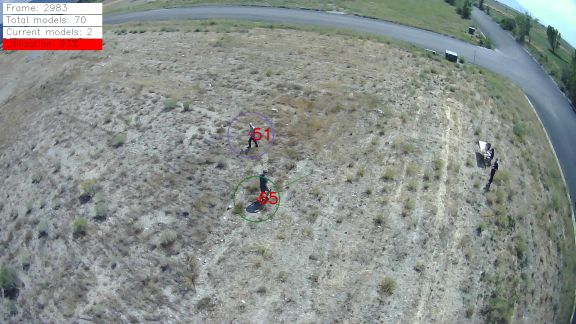
\includegraphics[width=0.95\textwidth]{images/chapter3/ID65_follow_begin.png}
		\caption{The human operator has commanded the UAV to follow track ID 65 ($t=35$ s)}
		\label{camera4}
	\end{subfigure}
	\centering
	\begin{subfigure}{0.48\linewidth}
		\centering
		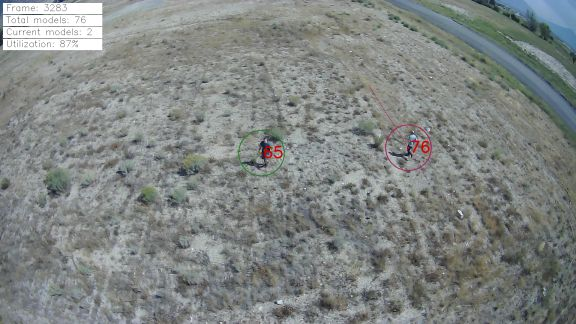
\includegraphics[width=\textwidth]{images/chapter3/ID65_following.png}
		\caption{A snapshot of the track ID 65 being followed ($t=60$ s)}
		\label{camera5}
	\end{subfigure}
	\caption{Camera view at various events}
	\label{camera}
\end{figure}
As shown in Figure \ref{camera1}, the human operator sees this camera view of multiple moving objects being tracked from the ground station and commands the multirotor to follow a target of interest by sending the correct track ID (Figure \ref{camera2}). The hardware test lasted about 1 minute and in the middle (t=35s) the operator commanded the multirotor to follow a different target (Figure \ref{camera4}). Until another track ID is commanded by the operator, the multirotor keeps following the current assigned target (Figure \ref{camera5}).

Figure \ref{image1} and \ref{image2} show the effort of the multirotor trying to place the target being followed in the center of the image plane. In Figure \ref{image1} and Figure \ref{image2}, the numbered events listed in Figure \ref{camera} are illustrated in the image plane. A track with ID 51 is initialized by the R-RANSAC tracker, and later the multirotor was commanded to follow track 51. The R-RANSAC tracker detected another moving object in the camera field of view and started to track the object with ID 65 while the multirotor was still following track 51. After a while, the human operator switches the target of interest resulting in the multirotor following track 65. The multirotor kept following the track 65 for the rest of the experiment. Finally, Figure \ref{gps} illustrates the GPS coordinates of the multirotor to show its movement and heading during the experiment. 

\begin{figure}[htbp]
	\centering
	\framebox{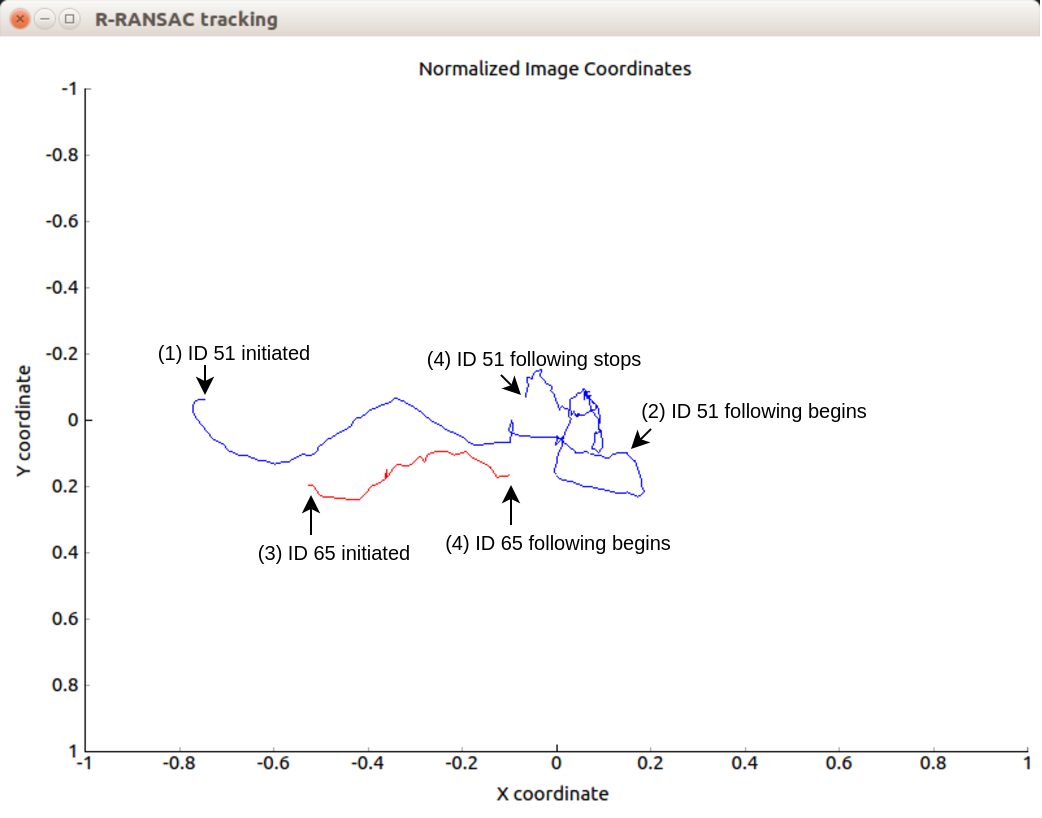
\includegraphics[height=7cm]{images/chapter3/ID65_follow_begin_annotated.png}}
	\caption[Tracks movement in the normalized image plane.]{Tracks movement in the normalized image plane. Each event (1)-(4) corresponds to camera view in \ref{camera1}-\ref{camera4} respectively. Until the command to follow ID 65, the multirotor keeps the track ID 51 from leaving the camera view.}
	\label{image1}
\end{figure}

\begin{figure}[htbp]
	\centering
	\framebox{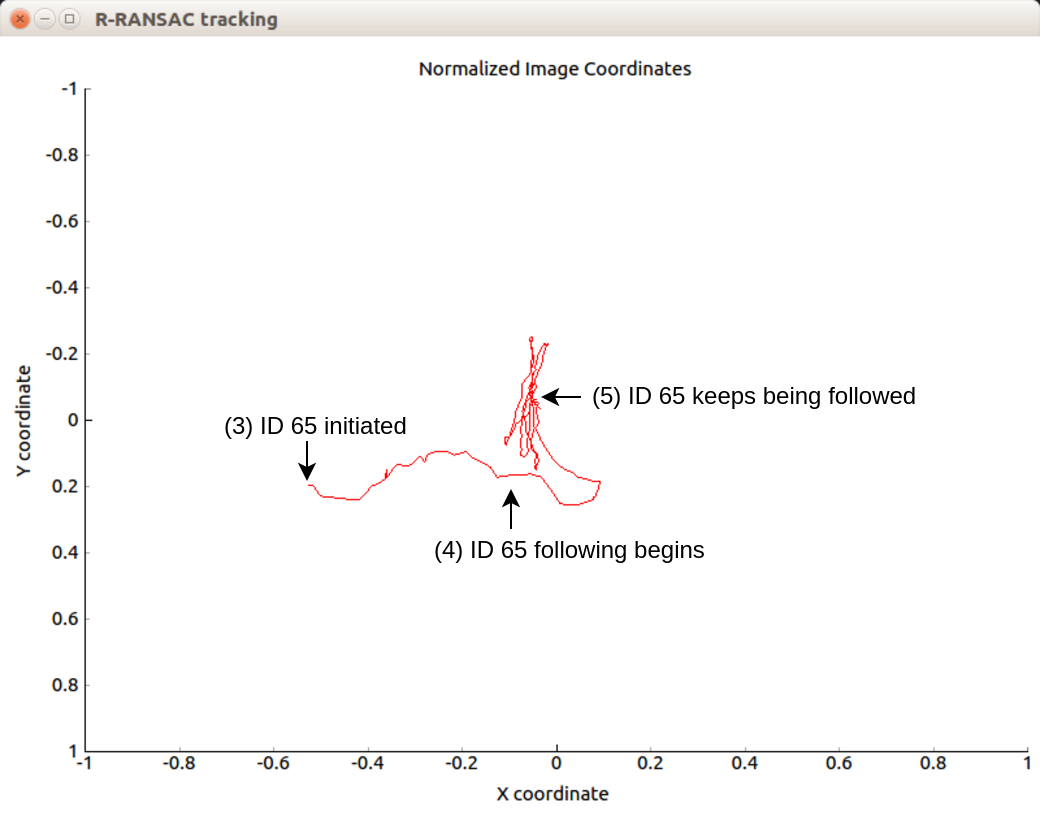
\includegraphics[height=7cm]{images/chapter3/ID65_trace_annotated.png}}
	\caption[The movement of track ID 65 in the normalized image plane.]{The movement of track ID 65 in the normalized image plane. Each event (3)-(5) corresponds to camera view in \ref{camera3}-\ref{camera5} respectively. The controller keeps the track ID 65 in the camera field of view after receiving the command to do so from the human operator.}
	\label{image2}
\end{figure}

\begin{figure}[htbp]
	\centering
	\framebox{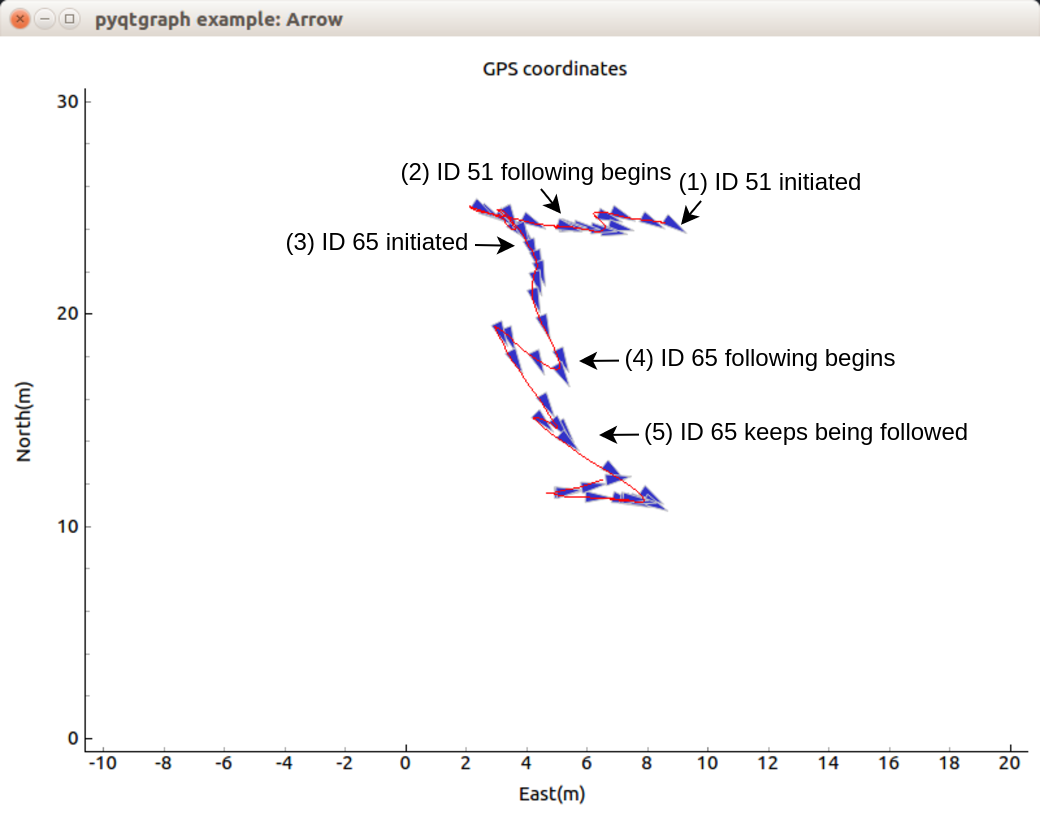
\includegraphics[height=7cm]{images/chapter3/GPS_trace.png}}
	\caption{Multirotor GPS footage and heading corresponding to camera view in \ref{camera1}-\ref{camera5} respectively.}
	\label{gps}
\end{figure}

\section{Conclusion}
In this chapter, a novel vision-based target following system with the R-RANSAC tracker is presented with hardware demonstration. The experimental result shows the feasibility of the real-time system in a realistic outdoor environment. With the R-RANSAC tracker, multiple moving objects in the camera view are tracked without having to know their colors or shapes. The controller is able to follow any particular target among the tracks with minimum effort to the human operator. The human operator is only expected to send a track ID number to the controller in order for the multirotor to follow the target of interest. This research opens up many other potential areas of research such as keeping multiple targets in the camera field of view, human machine interaction and multi UAS coordination in multiple target tracking situations.
\chapter{Unit Vector UAV Visual Servoing}
\label{chapter4}
\section{Motivation}
\begin{figure}[htbp]
	\centering
	\framebox{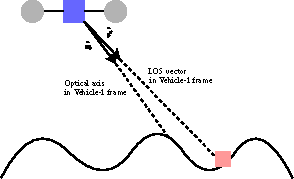
\includegraphics[width=0.6\textwidth]{images/chapter4/advanced_control_motivation.pdf}}
	\caption{Non-flat-earth model example. The unit optical axis vector $\hat{m}$ and the unit line of sight vector $\hat{\ell}$ are key components of the controller presented in this chapter.}
	\label{nonflatearth}
\end{figure}
The UAV control algorithm introduced in the previous chapter is relatively simple and easy to implement. However, the controller makes a strong assumption that can be unrealistic in some cases. For example, it assumes that the line of sight (LOS) vector to the target and the optical-axis terminate on the same flat surface, which is often called 'flat-earth assumption.' In that case, the altitude of the multirotor acts as a scale factor that can be used to compute how much the UAV should move forward. The more advanced UAV controller presented in this chapter overcomes the flat-earth assumption by working with the unit LOS vector and unit optical axis vector (see Figure \ref{nonflatearth}). Also, the controller does not require the altitude of the multirotor to be known because the scale factor does not have to be recovered.

\section{Unit Vector UAV Visual Servoing Derivation for Simple UAV Dynamics}
\begin{figure}[htbp]
	\centering
	\framebox{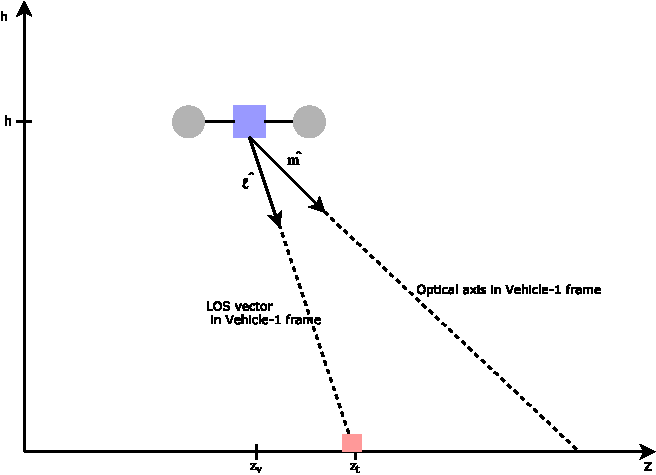
\includegraphics[width=0.6\textwidth]{images/chapter4/advanced_control_simple.pdf}}
	\caption{Graphical overview of the problem}
	\label{overview}
\end{figure}

As a first step in developing the control algorithm, we start with the simple vehicle dynamics  
\begin{equation}
\ddot{z}_v=u_1
\end{equation}
\begin{equation}
\ddot{h}=u_2,
\end{equation} 
where $z_v$ is multirotor's horizontal position and $h$ is its altitude as shown in Figure \ref{overview}.
A required input to the proposed controller is the measured unit LOS vector $\hat{\ell}$. 
Let $\hat{m}$ be the unit vector aligned with the optical axis, and let the projection matrix onto the null space of $\hat{m}$ be 
\begin{equation}
P_{\hat{m}}=(I-\hat{m}\hat{m}^\top).
\end{equation}
Selecting the coordinate frame as $(\hat{z},\ \hat{z}\times\hat{h},\ \hat{h})$, $\hat{m}$ can be represented as 
\begin{equation}
\hat{m}=\begin{pmatrix}
m_1 & 0 & -m_2
\end{pmatrix}^\top.
\end{equation}
In that case, we have 
\begin{align}
P_{\hat{m}}&=\begin{pmatrix}1 & 0 & 0 \\ 0 & 1 & 0 \\ 0 & 0 & 1 \end{pmatrix}
-\begin{pmatrix} m_1 \\ 0 \\ -m_2 \end{pmatrix}\begin{pmatrix} m_1 & 0 & -m_2 \end{pmatrix}
\\&=\begin{pmatrix}1-m_1^2 & 0 & m_1m_2 \\ 0 & 1 & 0 \\ m_1m_2 & 0 & 1-m_2^2 \end{pmatrix}.
\label{p_mhat}
\end{align}
Note that the controller is developed as if the multirotor is in 3D plane even if we only show 2D dynamics.
\begin{figure}[htbp]
	\centering
	\framebox{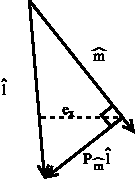
\includegraphics[width=0.2\textwidth]{images/chapter4/projection.pdf}}
	\caption{Projection onto the null space of the optical axis unit vector}
	\label{projection}
\end{figure}

The objective is to drive the horizontal component of $P_{\hat{m}}\hat{\ell}$ to zero (See Figure \ref{projection}). If we let
\begin{equation}
\hat{e}_1=[1 \quad 0 \quad 0]^\top,
\label{e_1}
\end{equation}
the horizontal component of $P_{\hat{m}}\hat{\ell}$ which is denoted by $e_x$ can be expressed as
\begin{equation}
e_x=\hat{e}_1^{\top}P_{\hat{m}}\hat{\ell}.
\end{equation}
Note that since $\hat{m}$ is fixed and known and $\hat{\ell}$ is measured, $e_x$ can also be measured. Also, since $\dot{\hat{\ell}}$ can be approximated by differentiating numerically,
\begin{equation}
\dot{e}_x=\hat{e}_1^{\top}P_{\hat{m}}\dot{\hat{\ell}}
\label{exdot}
\end{equation} is measurable.
Meanwhile, the line of sight vector is
\begin{equation}
\ell=\begin{pmatrix} z_t \\ 0 \\ 0 \end{pmatrix}
-\begin{pmatrix} z_v \\ 0 \\ h \end{pmatrix}.
\label{los}
\end{equation}
Differentiating equation (\ref{los}) gives 
\begin{equation}
\dot{\ell}=\begin{pmatrix} \dot{z}_t \\ 0 \\ 0 \end{pmatrix}
-\begin{pmatrix} \dot{z}_t \\ 0 \\ \dot{h} \end{pmatrix}
\end{equation}
and
\begin{equation}
\ddot{\ell}=\begin{pmatrix} \ddot{z}_t \\ 0 \\ 0 \end{pmatrix}
-\begin{pmatrix} \ddot{z}_v \\ 0 \\ \ddot{h} \end{pmatrix}.
\end{equation}
Assuming that the velocity of the target and the UAV altitude (i.e. $u_2=0$) are not changing yields
\begin{equation}
\ddot{\ell}=\begin{pmatrix} -\ddot{z}_v \\ 0 \\ 0 \end{pmatrix}
=\begin{pmatrix} -u_1 \\ 0 \\ 0 \end{pmatrix}.
\label{lddot}
\end{equation}
Thus, combining equations (\ref{p_mhat}), (\ref{e_1}) and (\ref{lddot})
results in 
\begin{equation}
\hat{e}_1^{\top}P_{\hat{m}}\ddot{\ell}=-(1-m_1^2)u_1.
\label{eplddot}
\end{equation}
Let
\begin{equation}
L=\norm{\ell}
\end{equation} be the unknown depth between the camera and the target, or the norm of the LOS vector. Then, the unit LOS vector is 
\begin{equation}
\hat{\ell}=\frac{\ell}{L}.
\label{lhat}
\end{equation}
Differentiating equation (\ref{lhat}) gives
\begin{equation}
\dot{\hat{\ell}}=\frac{\dot{\ell}L-\ell\dot{L}}{L^2}=\frac{\dot{\ell}}{L}-\hat{\ell}\bigg(\frac{\dot{L}}{L}\bigg).
\label{lhatdot}
\end{equation}
Differentiating again gives
\begin{align}
\ddot{\hat{\ell}}&=\frac{\ddot{\ell}L-\dot{\ell}\dot{L}}{L^2}-\dot{\hat{\ell}}\bigg(\frac{\dot{L}}{L}\bigg)-\hat{\ell}\bigg(\frac{\ddot{L}L-\dot{L}^2}{L^2}\bigg)
\\&=\frac{\ddot{\ell}}{L}-\bigg(\frac{\dot{\ell}}{L}\bigg)\bigg(\frac{\dot{L}}{L}\bigg)-\dot{\hat{\ell}}\bigg(\frac{\dot{L}}{L}\bigg)-\hat{\ell}\bigg(\frac{\ddot{L}}{L}\bigg)+\hat{\ell}\bigg(\frac{\dot{L}}{L}\bigg)^2.
\end{align}
Plugging in for $\frac{\dot{\ell}}{L}=\dot{\hat{\ell}}+\hat{\ell}\bigg(\frac{\dot{L}}{L}\bigg)$ from equation (\ref{lhatdot}) gives
\begin{equation}
\ddot{\hat{\ell}}=\frac{\ddot{\ell}}{L}-2\dot{\hat{\ell}}\bigg(\frac{\dot{L}}{L}\bigg)-\hat{\ell}\bigg(\frac{\ddot{L}}{L}\bigg).
\label{lhatddot}
\end{equation}
Differentiating equation (\ref{exdot}) and using equation (\ref{lhatddot}) for $\ddot{\hat{\ell}}$ yields
\begin{align}
\ddot{e}_x&=\hat{e}_1^{\top}P_{\hat{m}}\ddot{\hat{\ell}}
\\&=\hat{e}_1^{\top}P_{\hat{m}}\bigg(\frac{\ddot{\ell}}{L}-2\dot{\hat{\ell}}\bigg(\frac{\dot{L}}{L}\bigg)-\hat{\ell}\bigg(\frac{\ddot{L}}{L}\bigg)\bigg)
\\&=\frac{1}{L}(\hat{e}_1^{\top}P_{\hat{m}}\ddot{\ell})+\frac{\dot{L}}{L}(-2\hat{e}_1^{\top}P_{\hat{m}}\dot{\hat{\ell}})+\frac{\ddot{L}}{L}(-\hat{e}_1^{\top}P_{\hat{m}}\hat{\ell}).
\end{align}
Substituting (\ref{eplddot}) for $\hat{e_1}^{\top}P_{\hat{m}}\ddot{\ell}$ results in  
\begin{equation}
\ddot{e}_x=-\frac{1}{L}(1-m_1^2)u_1+\frac{\dot{L}}{L}(-2\hat{e}_1^{\top}P_{\hat{m}}\dot{\hat{\ell}})+\frac{\ddot{L}}{L}(-\hat{e}_1^{\top}P_{\hat{m}}\hat{\ell}).
\end{equation} 
Defining the unknown quantities
\begin{equation}
\beta_1\triangleq\frac{1}{L},\quad \beta_2\triangleq\frac{\dot{L}}{L}, \quad \beta_3\triangleq\frac{\ddot{L}}{L}
\end{equation}
and the measured quantities
\begin{equation}
\phi_1=1-m_1^2,\quad \phi_2=-2\hat{e}_1^{\top}P_{\hat{m}}\dot{\hat{\ell}}, \quad \phi_3=-\hat{e}_1^{\top}P_{\hat{m}}\hat{\ell},
\end{equation}
we can rewrite 
\begin{equation}
\ddot{e}_x=-\beta_1\phi_1u_1+\beta_2\phi_2+\beta_3\phi_3.
\label{exddot}
\end{equation}

In order to drive $e_x$ to zero, define
\begin{equation}
s=\dot{e}_x+ke_x,
\label{s}
\end{equation} where $k>0$. The reason why the equation (\ref{s}) is selected is because when $s\rightarrow0$, 
\begin{equation}
\dot{e}_x=-ke_x,
\end{equation} which makes $e_x$ asymptotically stable. Thus, if we can find the control input $u_1$ that makes $s\rightarrow0$, $e_x$ will converge to zero. Differentiating equation (\ref{s}) and substituting (\ref{exddot}) for $\ddot{e}_x$ yields
\begin{align}
\dot{s}&=\ddot{e}_x+k\dot{e}_x
\\&=-\beta_1\phi_1u_1+\beta_2\phi_2+\beta_3\phi_3+k\dot{e}_x.
\label{sdot}
\end{align}
If $\beta_1$, $\beta_2$, and $\beta_3$ are known, then the ideal control input would be 
\begin{equation}
u_1=\frac{1}{\beta_1\phi_1}(\beta_2\phi_2+\beta_3\phi_3+k\dot{e}_x+\alpha s),
\end{equation}
where $\alpha>0$.
Then, 
\begin{equation}
\dot{s}=-\alpha s,
\end{equation} 
which makes $s$ asymptotically stable. 
However, since we do not know $\beta_1$, $\beta_2$, and $\beta_3$, we use the control input
\begin{equation}
u_1=\frac{1}{\hat{\beta}_1\phi_1}(\hat{\beta}_2\phi_2+\hat{\beta}_3\phi_3+k\dot{e}_x+\alpha s),
\label{actualcontrol}
\end{equation}
where $\hat{\beta}_1$, $\hat{\beta}_2$, and $\hat{\beta}_3$ are the estimates of $\beta_1$, $\beta_2$, and $\beta_3$ respectively. 
In that case, we have
\begin{align}
\dot{s}&=-\beta_1\phi_1u_1+\hat{\beta}_1\phi_1u_1-\hat{\beta}_1\phi_1u_1+\beta_2\phi_2+\beta_3\phi_3+k\dot{e}_x
\label{sdot1}
\\&=-(\beta_1-\hat{\beta}_1)\phi_1u_1+(\beta_2-\hat{\beta}_2)\phi_2+(\beta_3-\hat{\beta}_3)\phi_3-\alpha s
\\&=-\tilde{\beta}_1\phi_1u_1+\tilde{\beta}_2\phi_2+\tilde{\beta}_3\phi_3-\alpha s
\\&=\tilde{B}^\top\Phi-\alpha s,
\label{sdot2}
\end{align}
where 
\begin{equation}
B\triangleq\begin{pmatrix}
\beta_1 \\ \beta_2 \\ \beta_3
\end{pmatrix}, \quad
\hat{B}\triangleq\begin{pmatrix} \hat{\beta}_1 \\ \hat{\beta}_2 \\ \hat{\beta}_3 \end{pmatrix}, \quad
\tilde{B}\triangleq B-\hat{B}, \quad 
\Phi \triangleq \begin{pmatrix} -\phi_1u_1 \\ \phi_2 \\ \phi_3 \end{pmatrix}.
\end{equation}
Selecting the Lyapunov function
\begin{equation}
V=\frac{1}{2}s^2+\frac{1}{2}\tilde{B}^\top \Gamma^{-1}\tilde{B},
\label{v}
\end{equation}
and differentiating with respect to time gives
\begin{align}
\dot{V}&=s\dot{s}+\tilde{B}^\top \Gamma^{-1}\dot{\tilde{B}}
\\&=s(\tilde{B}^\top\Phi-\alpha s)+\tilde{B}^\top \Gamma^{-1}\dot{\tilde{B}}
\\&=-\alpha s^2+\tilde{B}^\top(s\Phi+\Gamma^{-1}\dot{\tilde{B}}).
\label{vdot}
\end{align}
Assuming $B$ is roughly constant or slowly varying (i.e. $\dot{B}=0$), we have that $\dot{\tilde{B}}=-\dot{\hat{B}}$ implying that
\begin{equation}
\dot{V}=-\alpha s^2+\tilde{B}^\top(s\Phi-\Gamma^{-1}\dot{\hat{B}}).
\end{equation}
Therefore, by choosing $\dot{\hat{B}}=s\Gamma\Phi$, gives
\begin{equation}
\dot{V}=-\alpha s^2,
\end{equation}
which implies that $s$ is asymptotically stable. Thus, the original objective of stabilizing $e_x$ is achieved. This control scheme is simulated in Simulink and Figures \ref{simple_simulation} and \ref{another_simple_simulation} show the performance of the controller for one initial condition. 
\begin{figure}[htbp]
	\centering
	\begin{subfigure}[t]{0.45\linewidth}
		\includegraphics[width=\textwidth]{images/chapter4/simple_zero}
		\caption{when $t=0$ s}
	\end{subfigure}
	~ %add desired spacing between images, e. g. ~, \quad, \qquad, \hfill etc. 
	%(or a blank line to force the subfigure onto a new line)
	\begin{subfigure}[t]{0.45\linewidth}
		\includegraphics[width=\textwidth]{images/chapter4/simple_ten}
		\caption{when $t=10$ s}
	\end{subfigure}
	\begin{subfigure}[t]{0.8\linewidth}
		\centering
		\includegraphics[width=0.5\textwidth]{images/chapter4/simple_ex}
		\caption{The horizontal error between the unit LOS vector and the unit optical axis vector converges to zero.}
	\end{subfigure}	
	\caption{Simple UAV dynamics visual servoing Simulink simulation. The blue square is flying UAV at constant altitude and the red square is a target on the ground moving at 5 m/s. The initial UAV and target positions are [-10, 15] and [20, 0] respectively. Tuning parameters are set to $k=1$, $\Gamma=I_3$ (identity matrix), and $\alpha=1000$.}
	\label{simple_simulation}
\end{figure}

\begin{figure}[htbp]
	\centering
	\begin{subfigure}[t]{0.45\linewidth}
		\includegraphics[width=\textwidth]{images/chapter4/another_simple_zero}
		\caption{when $t=0$ s}
	\end{subfigure}
	~ %add desired spacing between images, e. g. ~, \quad, \qquad, \hfill etc. 
	%(or a blank line to force the subfigure onto a new line)
	\begin{subfigure}[t]{0.45\linewidth}
		\includegraphics[width=\textwidth]{images/chapter4/another_simple_ten}
		\caption{when $t=10$ s}
	\end{subfigure}
	\begin{subfigure}[t]{0.8\linewidth}
		\centering
		\includegraphics[width=0.5\textwidth]{images/chapter4/another_simple_ex}
		\caption{The horizontal error between the unit LOS vector and the unit optical axis vector converges to zero.}
	\end{subfigure}	
	\caption{Simple UAV dynamics visual servoing Simulink simulation. The blue square is flying UAV at constant altitude and the red square is a target on the ground moving at -5 m/s. The initial UAV and target positions are [10, 15] and [-10, 0] respectively. Tuning parameters are set to $k=1$, $\Gamma=I_3$ (identity matrix), and $\alpha=1000$.}
	\label{another_simple_simulation}
\end{figure}


\section{Backstepping Controller Derivation for Multirotor Dynamics}
\subsection{Derivation}
The multirotor dynamics expressed in vehicle-1 frame \cite{Beard2008} is given by 
\begin{equation}
\ddot{p}_x=-\cos\phi\sin\theta\frac{F}{m}
\label{pxddot}
\end{equation}
\begin{equation}
\ddot{p}_y=\sin\phi\frac{F}{m}
\end{equation}
\begin{equation}
\ddot{p}_z=g-\cos\phi\cos\theta\frac{F}{m}
\end{equation}
\begin{equation}
\ddot{\phi}=\frac{1}{J_x}\tau_{\phi}
\end{equation}
\begin{equation}
\ddot{\theta}=\frac{1}{J_y}\tau_{\theta}
\label{thetaddot}
\end{equation}
\begin{equation}
\ddot{\psi}=\frac{1}{J_z}\tau_{\psi},
\end{equation}
where $m$ is the mass of multirotor and $J_x$, $J_y$, and, $J_z$ are the moments of inertia. Also, $F$ and $\tau$ are force and torque produced by the propellers. For our specific control interest, we are only concerned with forward and backward motion of the multirotor involving only the equation (\ref{pxddot}) and (\ref{thetaddot}). We also assume that the altitude of the multirotor is controlled with a separate altitude controller and the roll of multirotor, $\phi$, is controlled to be zero which means that the multirotor is restricted from moving sideways. When the target moves left or right, the multirotor yaws to keep the target in the camera's view and it is assumed that there is a controller for this. Applying the above conditions and using small angle approximation to linearize, the equation (\ref{pxddot}) becomes 
\begin{equation}
\ddot{p}_x=-\frac{F_e}{m}\theta,
\end{equation}
where $F_e$ is the force to keep the multirotor in a constant altitude hover when the roll and pitch angles are zero. The line of sight vector is given by 
\begin{equation}
\ell=\begin{pmatrix}
p_x^{tar} \\ 0 \\ 0
\end{pmatrix}
-\begin{pmatrix}
p_x^{uav} \\ 0 \\ p_z^{uav}
\end{pmatrix}.
\label{l}
\end{equation}
Differentiating (\ref{l}) we get
\begin{equation}
\dot{\ell}=\begin{pmatrix}
\dot{p}_x^{tar} \\ 0 \\ 0
\end{pmatrix}
-\begin{pmatrix}
\dot{p}_x^{uav} \\ 0 \\ \dot{p}_z^{uav}
\end{pmatrix},
\label{ldot}
\end{equation}
and 
\begin{equation}
\ddot{\ell}=\begin{pmatrix}
\ddot{p}_x^{tar} \\ 0 \\ 0
\end{pmatrix}
-\begin{pmatrix}
\ddot{p}_x^{uav} \\ 0 \\ \ddot{p}_z^{uav}
\end{pmatrix}.
\label{lddot1}
\end{equation}
Referring back to (\ref{p_mhat}), (\ref{e_1}) and (\ref{lddot1}) we get that  
\begin{align}
\hat{e}_1^{\top}P_{\hat{m}}\ddot{\ell}&=(1-m_1^2)(\ddot{p}_x^{tar}-\ddot{p}_x^{uav})+m_1m_2\ddot{p}_z^{uav}
\\&=(1-m_1^2)\frac{F_e}{m}\theta
\end{align}
assuming that the multirotor keeps its altitude constant and the target does not accelerate. Notice that 
\begin{equation}
P_{\hat{m}}=\begin{pmatrix}1-m_1^2 & 0 & -m_1m_2 \\ 0 & 1 & 0 \\ -m_1m_2 & 0 & 1-m_2^2 \end{pmatrix},
\end{equation}
which is different from (\ref{p_mhat}) because now the $z$ component of the optical axis unit vector in vehicle-1 frame aligns with $z$ axis of the vehicle-1 frame (i.e. NED coordinate frame). However, this turns out to not affect the controller derivation.  Again, the control objective is to drive $e_x$ to zero and this can be achieved by driving $s=\dot{e_x}+ke_x$ to zero.
Recalling (\ref{exddot}) we get
\begin{align}
\ddot{e}_x&=\frac{1}{L}(1-m_1^2)\frac{F_e}{m}\theta+\frac{\dot{L}}{L}(-2\hat{e}_1^{\top}P_{\hat{m}}\dot{\hat{\ell}})+\frac{\ddot{L}}{L}(-\hat{e}_1^{\top}P_{\hat{m}}\hat{\ell})
\\&=\beta_1\phi_1\frac{F_e}{m}\theta+\beta_2\phi_2+\beta_3\phi_3,
\label{exddot1}
\end{align} 
where
\begin{equation}
\beta_1 \triangleq \frac{1}{L},\quad \beta_2 \triangleq \frac{\dot{L}}{L}, \quad \beta_3 \triangleq \frac{\ddot{L}}{L}
\end{equation}
and
\begin{equation}
\phi_1 \triangleq 1-m_1^2,\quad \phi_2 \triangleq -2\hat{e}_1^{\top}P_{\hat{m}}\dot{\hat{\ell}}, \quad \phi_3 \triangleq -\hat{e}_1^{\top}P_{\hat{m}}\hat{\ell}.
\end{equation}
Since we have all necessary components, we can get 
\begin{align}
\dot{s}&=\ddot{e}_x+k\dot{e}_x
\\&=\beta_1\phi_1\frac{F_e}{m}\theta+\beta_2\phi_2+\beta_3\phi_3+k\dot{e}_x.
\label{sdot3}
\end{align}
Manipulating (\ref{sdot3}) yields
\begin{align}
\dot{s}&=\beta_1\phi_1\frac{F_e}{m}\theta+\beta_2\phi_2+\beta_3\phi_3+k\dot{e_x}+\hat{\beta}_1\phi_1\frac{F_e}{m}\theta+\hat{\beta}_2\phi_2+\hat{\beta}_3\phi_3-\hat{\beta}_1\phi_1\frac{F_e}{m}\theta-\hat{\beta}_2\phi_2-\hat{\beta}_3\phi_3
\\&=(\beta_1-\hat{\beta}_1)\phi_1\frac{F_e}{m}\theta+(\beta_2-\hat{\beta}_2)\phi_2+(\beta_3-\hat{\beta}_3)\phi_3+k\dot{e_x}+\hat{\beta}_1\phi_1\frac{F_e}{m}\theta+\hat{\beta}_2\phi_2+\hat{\beta}_3\phi_3
\\&=\tilde{\beta}_1\phi_1\frac{F_e}{m}\theta+\tilde{\beta}_2\phi_2+\tilde{\beta}_3\phi_3+k\dot{e_x}+\hat{\beta}_1\phi_1\frac{F_e}{m}\theta+\hat{\beta}_2\phi_2+\hat{\beta}_3\phi_3
\\&=\tilde{B}^\top\Phi+k\dot{e_x}+\hat{\beta}_1\phi_1\frac{F_e}{m}\theta+\hat{\beta}_2\phi_2+\hat{\beta}_3\phi_3,
\end{align}
where 
\begin{equation}
B \triangleq \begin{pmatrix}
\beta_1 \\ \beta_2 \\ \beta_3
\end{pmatrix}, \quad
\hat{B} \triangleq \begin{pmatrix} \hat{\beta}_1 \\ \hat{\beta}_2 \\ \hat{\beta}_3 \end{pmatrix}, \quad
\tilde{B} \triangleq B-\hat{B}, \quad 
\Phi \triangleq \begin{pmatrix} \phi_1\frac{F_e}{m}\theta \\ \phi_2 \\ \phi_3 \end{pmatrix}.
\end{equation}
Define the Lyapunov function candidate as
\begin{equation}
V_1=\frac{1}{2}s^2+\frac{1}{2}\tilde{B}^\top \Gamma^{-1}\tilde{B}
\label{v1}
\end{equation}
and take the derivative to get
\begin{align}
\dot{V}_1&=s\dot{s}+\tilde{B}^\top \Gamma^{-1}\dot{\tilde{B}}
\\&=s(\tilde{B}^\top\Phi+k\dot{e_x}+\hat{\beta}_1\phi_1\frac{F_e}{m}\theta+\hat{\beta}_2\phi_2+\hat{\beta}_3\phi_3)+\tilde{B}^\top \Gamma^{-1}\dot{\tilde{B}}
\\&=s(k\dot{e_x}+\hat{\beta}_1\phi_1\frac{F_e}{m}\theta+\hat{\beta}_2\phi_2+\hat{\beta}_3\phi_3)+s\tilde{B}^\top\Phi+\tilde{B}^\top \Gamma^{-1}\dot{\tilde{B}}.
\label{sdot4}
\end{align}
Assuming that $B$ is constant or slowly changing, then $\dot{\tilde{B}}=-\dot{\hat{B}}$, and equation (\ref{sdot4}) becomes 
\begin{equation}
\dot{V}_1=s(k\dot{e_x}+\hat{\beta}_1\phi_1\frac{F_e}{m}\theta+\hat{\beta}_2\phi_2+\hat{\beta}_3\phi_3)+s\tilde{B}^\top\Phi-\tilde{B}^\top \Gamma^{-1}\dot{\hat{B}}.
\end{equation}
By selecting $\dot{\hat{B}}=s\Gamma\Phi$, the above equation further becomes 
\begin{equation}
\dot{V}_1=s(k\dot{e_x}+\hat{\beta}_1\phi_1\frac{F_e}{m}\theta+\hat{\beta}_2\phi_2+\hat{\beta}_3\phi_3).
\label{v1dot}
\end{equation}
For some cases, $\theta$ is the direct control input that can be commanded making the problem less complicated. However, for the multirotor dynamics, $\theta$ is indirectly controlled by torque $\tau_\theta$ which leads to the development of backstepping control technique. The backstepping control is especially useful when the system has cascaded structure such as this multirotor case by using some of the state variables as pseudo controls to backstep until the final external control input is reached. With backstepping, a Lyapunov function is derived for the entire system \cite{khalil1996noninear}, \cite{raptis2010linear}. We start by adding and subtracting a pseudo control $\xi_1$ to equation (\ref{v1dot}) as
\begin{equation}
\dot{V}_1=s(k\dot{e_x}+\hat{\beta}_1\phi_1\frac{F_e}{m}\theta+\hat{\beta}_2\phi_2+\hat{\beta}_3\phi_3+\xi_1-\xi_1).
\end{equation}
By selecting $\xi_1=-k\dot{e}_x-\hat{\beta}_2\phi_2-\hat{\beta}_3\phi_3-k_1s$, 
\begin{equation}
\dot{V}_1=-k_1s^2+ s(\hat{\beta}_1\phi_1\frac{F_e}{m}\theta-\xi_1).
\label{v2dot}
\end{equation}
Define a new Lyapunov function candidate as
\begin{equation}
V_2=V_1+\frac{1}{2}(\hat{\beta}_1\phi_1\frac{F_e}{m}\theta-\xi_1)^2,
\label{v2}
\end{equation}
and taking derivative, we get
\begin{align}
\dot{V}_2&=\dot{V}_1+(\hat{\beta}_1\phi_1\frac{F_e}{m}\theta-\xi_1)(\phi_1\frac{F_e}{m}(\dot{\hat{\beta}}_1\theta+\hat{\beta}_1\dot{\theta})-\dot{\xi}_1)
\\&=-k_1s^2+
(\hat{\beta}_1\phi_1\frac{F_e}{m}\theta-\xi_1)
(s+\phi_1\frac{F_e}{m}(\dot{\hat{\beta}}_1\theta+\hat{\beta}_1\dot{\theta})-\dot{\xi}_1+\xi_2-\xi_2).
\end{align}
Assigning $\xi_2=\dot{\xi}_1-s-\phi_1\frac{F_e}{m}\dot{\hat{\beta}}_1\theta-k_2(\hat{\beta}_1\phi_1\frac{F_e}{m}\theta-\xi_1)$ leads to
\begin{equation}
\dot{V}_2=-k_1s^2-k_2(\hat{\beta}_1\phi_1\frac{F_e}{m}\theta-\xi_1)^2+
(\hat{\beta}_1\phi_1\frac{F_e}{m}\theta-\xi_1)
(\phi_1\frac{F_e}{m}\hat{\beta}_1\dot{\theta}-\xi_2).
\label{v2dotfinal}
\end{equation}
Finally, define a new Lyapunov function as 
\begin{equation}
V_3=V_2+\frac{1}{2}(\phi_1\frac{F_e}{m}\hat{\beta}_1\dot{\theta}-\xi_2)^2,
\label{v3}
\end{equation}
and differentiate to get
\begin{align}
\dot{V}_3&=\dot{V}_2+
(\phi_1\frac{F_e}{m}\hat{\beta}_1\dot{\theta}-\xi_2)
(\phi_1\frac{F_e}{m}\dot{\hat{\beta}}_1\dot{\theta}+\phi_1\frac{F_e}{m}\hat{\beta}_1\ddot{\theta}-\dot{\xi}_2)
\\&=-k_1s^2-k_2(\hat{\beta}_1\phi_1\frac{F_e}{m}\theta-\xi_1)^2+(\phi_1\frac{F_e}{m}\hat{\beta}_1\dot{\theta}-\xi_2)
(\hat{\beta}_1\phi_1\frac{F_e}{m}\theta-\xi_1+\phi_1\frac{F_e}{m}\dot{\hat{\beta}}_1\dot{\theta}+\phi_1\frac{F_e}{m}\hat{\beta}_1\ddot{\theta}-\dot{\xi}_2).
\label{v3dot}
\end{align}
 Using the relationship between the angular acceleration and torque in (\ref{thetaddot}), the above equation becomes
\begin{equation}
\dot{V}_3=-k_1s^2-k_2(\hat{\beta}_1\phi_1\frac{F_e}{m}\theta-\xi_1)^2+(\phi_1\frac{F_e}{m}\hat{\beta}_1\dot{\theta}-\xi_2)
(\hat{\beta}_1\phi_1\frac{F_e}{m}\theta-\xi_1+\phi_1\frac{F_e}{m}\dot{\hat{\beta}}_1\dot{\theta}+\phi_1\frac{F_e}{m}\hat{\beta}_1\frac{1}{J_y}\tau_\theta-\dot{\xi}_2).
\label{v3dotfinal}
\end{equation}
Notice that $\tau_\theta$ finally showed up in the equation (\ref{v3dotfinal}) which we can directly control. Thus, by setting 
\begin{equation}
\tau_\theta=\frac{J_ym}{\phi_1F_e\hat{\beta}_1}
(\xi_1+\dot{\xi}_2-\hat{\beta}_1\phi_1\frac{F_e}{m}\theta-\phi_1\frac{F_e}{m}\dot{\hat{\beta}}_1\dot{\theta}-k_3(\phi_1\frac{F_e}{m}\hat{\beta}_1\dot{\theta}-\xi_2)),
\end{equation}
gives
\begin{equation}
\dot{V}_3=-k_1s^2-k_2(\hat{\beta}_1\phi_1\frac{F_e}{m}\theta-\xi_1)^2-k_3(\phi_1\frac{F_e}{m}\hat{\beta}_1\dot{\theta}-\xi_2)^2.
\end{equation}
Because of the cascaded structure of the backstepping control, the fact that $V_3(t)\rightarrow 0$ means that $V_1(t)$ also converges to zero.

\subsection{Simulation}
The backstepping control algorithm derived above is simulated in Simulink with more realistic multirotor dynamics that can be found in {\cite{Beard2008}}. The simulation only tests the forward motion control of the multirotor by having separate PID controller to keep roll and yaw motions unmoved. There are two types of backstepping controller tested. Both cases the same backstepping controller is used and it only requires the unit optical axis vector and unit LOS vector as inputs to compute the multirotor pitch torque output. The first is using the inertial LOS vector and normalize it to get the unit LOS vector shown in Figure \ref{system_inertial}. This is rather unrealistic because it is usually not feasible to know the target location in the inertial frame to get the inertial LOS vector. However, this is still tested as an intermediate step and is used to test the validity of the backstepping control algorithm itself. The simulation results with various target velocity 0 m/s, 5 m/s, and -5 m/s can be found in Figure \ref{inertial_0mps}, \ref{inertial_5mps}, and \ref{inertial_-5mps} respectively. Figure \ref{inertial_0mps} shows that the backstepping controller is capable of keeping the static target in the camera's field of view using the unit vector visual servoing framework. Also, the horizontal error between the unit LOS vector and the unit optical axis vector both in the vehicle-1 frame converges to zero. Figure \ref{inertial_5mps} and \ref{inertial_-5mps} show that the backstepping controller can keep the target moving at 5 m/s and -5 m/s in the camera's view. In both cases, the target is not placed at the center of image because the horizontal error is computed in the vehicle-1 frame meaning that the pitch of multirotor is not compensated. In the future with further research, the target can be placed at the image center by adding a simple pitch gimbal. 
\begin{figure}[htbp]
	\centering
	\framebox{\includegraphics[width=0.8\textwidth]{images/chapter4/inertial_LOS_backstepping.pdf}}
	\caption{Control system diagram for the inertial line of sight vector backstepping controller. In this configuration, the backstepping controller needs the positions of multirotor and target.}
	\label{system_inertial}
\end{figure}

\begin{figure}[htbp]
	\centering
	\framebox{\includegraphics[width=0.8\textwidth]{images/chapter4/image_based_backstepping.pdf}}
	\caption{Control system diagram for the image-based backstepping controller. Note that the backstepping controller only requires the image coordinates of the target.}
	\label{system_image}
\end{figure}

\begin{figure}[htbp]
	\centering
	\begin{subfigure}[t]{0.45\linewidth}
		\includegraphics[width=\textwidth]{images/chapter4/inertial_UAV_0mps}
		\caption{Multirotor and ground target when $t=0$ s}
	\end{subfigure}
	\begin{subfigure}[t]{0.45\linewidth}
		\includegraphics[width=\textwidth]{images/chapter4/inertial_UAV_0mps_60s}
		\caption{when $t=60$ s}
	\end{subfigure}
	\begin{subfigure}[t]{0.45\linewidth}
		\includegraphics[width=\textwidth]{images/chapter4/inertial_camera_0mps}
		\caption{Camera view when $t=0$ s}
	\end{subfigure}
	\begin{subfigure}[t]{0.45\linewidth}
		\includegraphics[width=\textwidth]{images/chapter4/inertial_camera_0mps_60s}
		\caption{when $t=60$ s}
	\end{subfigure}
	\begin{subfigure}[t]{0.8\linewidth}
		\centering
		\includegraphics[width=0.5\textwidth]{images/chapter4/inertial_Ex_0mps}
		\caption{The horizontal error ($e_x$) between the unit LOS vector and the unit optical axis vector both in the vehicle-1 frame converges to zero. It saturates at 0.05 to prevent the multirotor from commanding too large torque command.}
	\end{subfigure}	
	\caption{Simulation result for the backstepping control using the inertial LOS vector. The ground target is static (0 m/s). The initial UAV and target positions are [-140, 0, -90] and [0, 0, 0] respectively. Tuning parameters are set to $k=0.12$, $k_1=1$, $k_2=1$, $k_3=1$, and $\Gamma=0.01I_3$ (identity matrix).}
	\label{inertial_0mps}
\end{figure}

\begin{figure}[htbp]
	\centering
	\begin{subfigure}[t]{0.32\linewidth}
		\includegraphics[width=\textwidth]{images/chapter4/inertial_UAV_5mps}
		\caption{when $t=0$ s}
	\end{subfigure}
	\begin{subfigure}[t]{0.32\linewidth}
		\includegraphics[width=\textwidth]{images/chapter4/inertial_UAV_5mps_90s}
		\caption{when $t=90$ s}
	\end{subfigure}
	\begin{subfigure}[t]{0.32\linewidth}
		\includegraphics[width=\textwidth]{images/chapter4/inertial_UAV_5mps_180s}
		\caption{when $t=180$ s}
	\end{subfigure}
	\begin{subfigure}[t]{0.32\linewidth}
		\includegraphics[width=\textwidth]{images/chapter4/inertial_camera_5mps}
		\caption{when $t=0$ s}
	\end{subfigure}
	\begin{subfigure}[t]{0.32\linewidth}
		\includegraphics[width=\textwidth]{images/chapter4/inertial_camera_5mps_90s}
		\caption{when $t=90$ s}
	\end{subfigure}
	\begin{subfigure}[t]{0.32\linewidth}
		\includegraphics[width=\textwidth]{images/chapter4/inertial_camera_5mps_180s}
		\caption{when $t=180$ s}
	\end{subfigure}	
	\begin{subfigure}[t]{0.8\linewidth}
		\centering
		\includegraphics[width=0.5\textwidth]{images/chapter4/inertial_Ex_5mps}
		\caption{The horizontal error ($e_x$) between the unit LOS vector and the unit optical axis vector both in the vehicle-1 frame converges to zero. It saturates at 0.05 to prevent the multirotor from commanding too large torque command.}
	\end{subfigure}	
	\caption{Simulation result for the backstepping control using the inertial LOS vector. The ground target is moving at the speed of 5 m/s. The initial UAV and target positions are [-110, 0, -90] and [0, 0, 0] respectively. Tuning parameters are set to $k=0.12$, $k_1=1$, $k_2=1$, $k_3=1$, and $\Gamma=0.01I_3$ (identity matrix). In this case, the target is not placed at the center of image because the horizontal error is computed in the vehicle-1 frame meaning that the pitch of multirotor is not compensated.}
	\label{inertial_5mps}
\end{figure}

\begin{figure}[htbp]
	\centering
	\begin{subfigure}[t]{0.32\linewidth}
		\includegraphics[width=\textwidth]{images/chapter4/inertial_UAV_-5mps}
		\caption{when $t=0$ s}
	\end{subfigure}
	\begin{subfigure}[t]{0.32\linewidth}
		\includegraphics[width=\textwidth]{images/chapter4/inertial_UAV_-5mps_90s}
		\caption{when $t=90$ s}
	\end{subfigure}
	\begin{subfigure}[t]{0.32\linewidth}
		\includegraphics[width=\textwidth]{images/chapter4/inertial_UAV_-5mps_180s}
		\caption{when $t=180$ s}
	\end{subfigure}
	\begin{subfigure}[t]{0.32\linewidth}
		\includegraphics[width=\textwidth]{images/chapter4/inertial_camera_-5mps}
		\caption{when $t=0$ s}
	\end{subfigure}
	\begin{subfigure}[t]{0.32\linewidth}
		\includegraphics[width=\textwidth]{images/chapter4/inertial_camera_-5mps_90s}
		\caption{when $t=90$ s}
	\end{subfigure}
	\begin{subfigure}[t]{0.32\linewidth}
		\includegraphics[width=\textwidth]{images/chapter4/inertial_camera_-5mps_180s}
		\caption{when $t=180$ s}
	\end{subfigure}	
	\begin{subfigure}[t]{0.8\linewidth}
		\centering
		\includegraphics[width=0.5\textwidth]{images/chapter4/inertial_Ex_-5mps}
		\caption{The horizontal error ($e_x$) between the unit LOS vector and the unit optical axis vector both in the vehicle-1 frame converges to zero. It saturates at 0.05 to prevent the multirotor from commanding too large torque command.}
	\end{subfigure}	
	\caption{Simulation result for the backstepping control using the inertial LOS vector. The ground target is moving at the speed of -5 m/s. The initial UAV and target positions are [-110, 0, -90] and [0, 0, 0] respectively. Tuning parameters are set to $k=0.12$, $k_1=1$, $k_2=1$, $k_3=1$, and $\Gamma=0.01I_3$ (identity matrix). In this case, the target is not placed at the center of image because the horizontal error is computed in the vehicle-1 frame meaning that the pitch of multirotor is not compensated.}
	\label{inertial_-5mps}
\end{figure}

The second backstepping controller is the actual simulation of the hardware demonstration. When the multirotor is equipped with monocular camera only, the multirotor has no other way to know where the target is relative to itself but through the information received from the camera. Thus, the second controller is only using the camera information (target pixel location) to control the multirotor (See Figure \ref{system_image}). The camera is simulated to output its information at 30 Hz while the backstepping controller is evaluated at 100 Hz. This caused the horizontal error $e_x$ to be quite noisy which eventually makes the controller unstable. Thus, a low-pass filter is added internally in the backstepping controller to smooth $e_x$. The simulation results for a static target, moving targets at 5 m/s and -5 m/s can be found in Figure \ref{image_0mps}, \ref{image_5mps}, and \ref{image_-5mps} respectively. In Figure \ref{image_0mps}, the target is kept in the camera FOV and the horizontal error converges to zero. Figure \ref{image_5mps} and \ref{image_-5mps} show not much different results from Figure \ref{inertial_5mps} and \ref{inertial_-5mps} showing almost identical target location in the image and the horizontal error trend over time. 

In conclusion, based on the comparison between the inertial LOS vector (100 Hz update rate) and the image LOS vector (30 Hz update rate) as inputs to the backstepping controller, it turns out that there is no significant performance decrease using the sparse image information compared to using the inertial LOS vector directly as long as a simple low-pass filter is implemented internally in the backstepping controller to smooth the jittery horizontal error ($e_x$). Thus, the proposed controller can be tested in hardware using a multirotor equipped with monocular camera.

\begin{figure}[htbp]
	\centering
	\begin{subfigure}[t]{0.45\linewidth}
		\includegraphics[width=\textwidth]{images/chapter4/image_UAV_0mps}
		\caption{Multirotor and ground target when $t=0$ s}
	\end{subfigure}
	\begin{subfigure}[t]{0.45\linewidth}
		\includegraphics[width=\textwidth]{images/chapter4/image_UAV_0mps_60s}
		\caption{when $t=60$ s}
	\end{subfigure}
	\begin{subfigure}[t]{0.45\linewidth}
		\includegraphics[width=\textwidth]{images/chapter4/image_camera_0mps}
		\caption{Camera view when $t=0$ s}
	\end{subfigure}
	\begin{subfigure}[t]{0.45\linewidth}
		\includegraphics[width=\textwidth]{images/chapter4/image_camera_0mps_60s}
		\caption{when $t=60$ s}
	\end{subfigure}
	\begin{subfigure}[t]{0.8\linewidth}
		\centering
		\includegraphics[width=0.5\textwidth]{images/chapter4/image_Ex_0mps}
		\caption{The horizontal error ($e_x$) between the normalized target pixel coordinates and the unit optical axis vector both in the vehicle-1 frame converges to zero. Note that the value is low-pass filtered.}
	\end{subfigure}	
	\caption{Simulation result for the backstepping control using the normalized target pixel coordinates. The ground target is static (0 m/s). The initial UAV and target positions are [-140, 0, -90] and [0, 0, 0] respectively. Tuning parameters are set to $k=0.12$, $k_1=1$, $k_2=1$, $k_3=1$, and $\Gamma=0.01I_3$ (identity matrix).}
	\label{image_0mps}
\end{figure}

\begin{figure}[htbp]
	\centering
	\begin{subfigure}[t]{0.32\linewidth}
		\includegraphics[width=\textwidth]{images/chapter4/image_UAV_5mps}
		\caption{when $t=0$ s}
	\end{subfigure}
	\begin{subfigure}[t]{0.32\linewidth}
		\includegraphics[width=\textwidth]{images/chapter4/image_UAV_5mps_90s}
		\caption{when $t=90$ s}
	\end{subfigure}
	\begin{subfigure}[t]{0.32\linewidth}
		\includegraphics[width=\textwidth]{images/chapter4/image_UAV_5mps_180s}
		\caption{when $t=180$ s}
	\end{subfigure}
	\begin{subfigure}[t]{0.32\linewidth}
		\includegraphics[width=\textwidth]{images/chapter4/image_camera_5mps}
		\caption{when $t=0$ s}
	\end{subfigure}
	\begin{subfigure}[t]{0.32\linewidth}
		\includegraphics[width=\textwidth]{images/chapter4/image_camera_5mps_90s}
		\caption{when $t=90$ s}
	\end{subfigure}
	\begin{subfigure}[t]{0.32\linewidth}
		\includegraphics[width=\textwidth]{images/chapter4/image_camera_5mps_180s}
		\caption{when $t=180$ s}
	\end{subfigure}	
	\begin{subfigure}[t]{0.8\linewidth}
		\centering
		\includegraphics[width=0.5\textwidth]{images/chapter4/image_Ex_5mps}
		\caption{The horizontal error ($e_x$) between the normalized target pixel coordinates and the unit optical axis vector both in the vehicle-1 frame converges to zero. Note that the value is low-pass filtered.}
	\end{subfigure}	
	\caption{Simulation result for the backstepping control using the normalized target pixel coordinates. The ground target is moving at the speed of 5 m/s. The initial UAV and target positions are [-110, 0, -90] and [0, 0, 0] respectively. Tuning parameters are set to $k=0.12$, $k_1=1$, $k_2=1$, $k_3=1$, and $\Gamma=0.01I_3$ (identity matrix). In this case, the target is not placed at the center of image because the horizontal error is computed in the vehicle-1 frame meaning that the pitch of multirotor is not compensated.}
	\label{image_5mps}
\end{figure}

\begin{figure}[htbp]
	\centering
	\begin{subfigure}[t]{0.32\linewidth}
		\includegraphics[width=\textwidth]{images/chapter4/image_UAV_-5mps}
		\caption{when $t=0$ s}
	\end{subfigure}
	\begin{subfigure}[t]{0.32\linewidth}
		\includegraphics[width=\textwidth]{images/chapter4/image_UAV_-5mps_90s}
		\caption{when $t=90$ s}
	\end{subfigure}
	\begin{subfigure}[t]{0.32\linewidth}
		\includegraphics[width=\textwidth]{images/chapter4/image_UAV_-5mps_180s}
		\caption{when $t=180$ s}
	\end{subfigure}
	\begin{subfigure}[t]{0.32\linewidth}
		\includegraphics[width=\textwidth]{images/chapter4/image_camera_-5mps}
		\caption{when $t=0$ s}
	\end{subfigure}
	\begin{subfigure}[t]{0.32\linewidth}
		\includegraphics[width=\textwidth]{images/chapter4/image_camera_-5mps_90s}
		\caption{when $t=90$ s}
	\end{subfigure}
	\begin{subfigure}[t]{0.32\linewidth}
		\includegraphics[width=\textwidth]{images/chapter4/image_camera_-5mps_180s}
		\caption{when $t=180$ s}
	\end{subfigure}	
	\begin{subfigure}[t]{0.8\linewidth}
		\centering
		\includegraphics[width=0.5\textwidth]{images/chapter4/image_Ex_-5mps}
		\caption{The horizontal error ($e_x$) between the normalized target pixel coordinates and the unit optical axis vector both in the vehicle-1 frame converges to zero. Note that the value is low-pass filtered.}
	\end{subfigure}	
	\caption{Simulation result for the backstepping control using the normalized target pixel coordinates. The ground target is moving at the speed of -5 m/s. The initial UAV and target positions are [-110, 0, -90] and [0, 0, 0] respectively. Tuning parameters are set to $k=0.12$, $k_1=1$, $k_2=1$, $k_3=1$, and $\Gamma=0.01I_3$ (identity matrix). In this case, the target is not placed at the center of image because the horizontal error is computed in the vehicle-1 frame meaning that the pitch of multirotor is not compensated.}
	\label{image_-5mps}
\end{figure}
%%%%%%%%%%%%% begin Bibliography %%%%%%%%%%%%%%%%%
\cleardoublepage
\bibliographystyle{IEEEtran}
\bibliography{references/refs} % Use your own BibTex file here

% Include appendix sections here: (or comment these lines out to have no appendices)
\appendix
\chapter{Making a Figure with Width Based on Page Size}
\label{apdx:appendixa}

\section{Width Based on Page Size Figure Example} \label{sec:appendixa_figure_example}
Here's an example of a figure whose width depends on the width
of the page. You can see it as Figure~\ref{fig:appendix_some_pic}. This also shows another citation \cite{aeyels86local}.

\begin{figure}[htbp]
  \centering
  \includegraphics[width=0.45\textwidth]{images/some_pic}
  \caption[Example figure whose width depends on page size]{
    This is an example of a figure whose width will be 45\% of the
    width of the page. If you'd like to see a figure with a fixed
    width then you can see it as Figure~\ref{fig:intro_stuff} in
    Section~\ref{sec:intro_figure_example} of Chapter~\ref{chp:chapter1}.}
  \label{fig:appendix_some_pic}
\end{figure}
\chapter{Formatting Guidelines for Thesis}
\label{apdx:appendixb}

This appendix outlines the required formatting for theses and dissertations. While the \LaTeX\ template takes care of most of these automatically, it is the student's responsibility to ensure that all formatting requirements are incorporated in the document.

\section{Font} Times New Roman 12 pt. throughout text and 10 or 11 point for tables and figures.

\section{Margins}
\begin{itemize}
\item Preliminary Pages (Title page, Abstract page(s), Acknowledgment page, Table of Contents, List of Figures, List of Tables):
1 inch on all sides
\item Body Pages, beginning with Introduction:
1 inch on all sides
\item Chapter title pages, Appendix title page, Reference title page:
2 inches at top,
1 inch at bottom and sides
\end{itemize}

\section{Printing}
\begin{itemize}
\item Single-sided: Title page, Abstract page(s), Acknowledgment page
\item Two-sided:  Table of Contents, List of Figures, List of Tables, Body, Appendix, References
\end{itemize}
Note:  Table of Contents, List of Figures, List of Tables, Chapter title pages, References and Appendix pages must begin on the front side of a page.

\section{Page Numbering}
\begin{itemize}
\item	Page numbers are centered at the bottom of the page.
\item	Counting begins with the Title page; however, back pages are not counted until the Table of Contents.
\item	Page numbers do not appear on the page until the Table of Contents (v).
\item	Use Roman Numerals (v, vi, vii, ...) for the Table of Contents page and the pages thereafter until Chapter 1.  
\item	Use Arabic numbers (1, 2, 3 ...) beginning with Chapter 1. 
\item	Be sure numbers appear on all blank back pages once numbering begins.
\end{itemize}

\section{Spacing}
\begin{itemize}
\item	Double-space text of body.
\item	Single-space abstract, captions, quotes, long chapter titles, headings, and subheadings.
\item	Table of Contents, List of Figures, List of Tables, and References can be single-spaced or double spaced.
\item	Double-space three times after chapter titles (48 pts).
\item	Double-space twice before subheadings (24 pts). 
\item	Double-space once after subheadings (0 pts). 
\item	Double-space once between two subheadings (0 pts). 
\item	Double-space twice before and after figures (24 pts).
\item	Double-space twice before and after tables (24 pts).
\item	Double-space once before and after equations (0 pts).
\item	Do not leave a single line of text, a single-line equation, or a subheading alone on the top (widow) or bottom (orphan) of a page.
\item	Do not leave more than about 5 lines of white space remaining on a page unless it�s the end of a chapter.
\end{itemize}

\section{Figures}
\begin{itemize}
\item	Figures are normally diagrams, graphs, maps, or charts.
\item	Center figures on the page.
\item	Center captions below the figure. If two lines are needed, the caption should be left justified at margin.
\item	A figure should be placed after the paragraph of reference.  If it will not fit on the same page, continue the text and place the figure on the next page.
\end{itemize}

\section{Tables}
\begin{itemize}
\item	Tables contain numerical or statistical information.
\item	Center tables on the page.
\item	Center captions above the table.  If more than one line is needed, center the lines in an inverted pyramid:                                                          
\begin{singlespace}
\begin{center}Table 6.3 Comparison of roll rotation plots when node was displaced,\\
 and an X-direction off-axis force was applied.\end{center}
\end{singlespace}
\item	If placed in the landscape position, the top of the table should be on the left side of the page, with the caption above the table.  The page number is placed in the standard location.
\end{itemize}

\end{document}